% !TeX TXS-program:compile = txs:///pdflatex/[--shell-escape]

% Clase del documento
\documentclass[11pt,twoside,titlepage]{report}

% Configuración
\include{config/config.tex}
\usepackage{graphicx}
\usepackage{svg}

% A rellenar por el estudiante
\newcommand{\nombreautor}{David Moreno Martín}
\newcommand{\nombretutor}{Micael Gallego Carrillo}
\newcommand{\titulotrabajo}{LogArt: Galería de recuerdos }
\newcommand{\grado}{Grado en Ingeniería del Software}
\newcommand{\curso}{Curso 2024-2025}

%%%%%%%%%%%%%%%%%%%%%%%%%%%%%%%%%%%%%%%%%%%%%%%%%%%%%%%%%%%%%%%%%%%%%%%
%                           Inicio del documento                       
%%%%%%%%%%%%%%%%%%%%%%%%%%%%%%%%%%%%%%%%%%%%%%%%%%%%%%%%%%%%%%%%%%%%%%%

\begin{document}

\pagestyle{plain}

%%%%%%%%%%%%%%%%%%%%%%%%%%%%%%%%%%%% Portada %%%%%%%%%%%%%%%%%%%%%%%%%%%%%%%%%%

\include{config/portada}

%%%%%%%%%%%%%%%%%%%%%%%%%%%%%%%%%%%%%%%%%%%%%%%%%%%%%%%%%%%%%%%%%%%%%%%%%%%%%%%

% Estilo de párrafo de los capítulos
\setlength{\parskip}{0.75em}
\renewcommand{\baselinestretch}{1.25}
% Interlineado simple
\spacing{1}

\pagenumbering{Roman}
\setcounter{page}{2}

%%%%%%%%%%%%%%%%%%%%%%%%% Licencia %%%%%%%%%%%%%%%%%%%%%%%%%%%

\include{config/licencia}

%%%%%%%%%%%%%%%%%%%%%%%%% Agradecimientos o dedicatoria %%%%%%%%%%%%%%%%%%%%%%%%%%%

\chapter*{Agradecimientos}

Quiero agradecer, en primer lugar, a mi familia, por estar siempre ahí, por apoyarme cuando pensaba dejarlo, por su apoyo constante y por darme la tranquilidad necesaria para poder llegar hasta aquí.

A mis amigos, por acompañarme durante este camino y por recordarme que siempre hay tiempo para desconectar, y que esa desconexión también es necesaria.

También quiero expresar mi agradecimiento a todos los profesores que, a lo largo de la carrera, han contribuido a mi formación académica y personal, incluyendo a mi tutor del Trabajo de Fin de Grado, Micael Gallego, por su guía, sus consejos y su implicación durante el desarrollo de este proyecto.

Este trabajo no habría sido posible sin todas estas personas.




\afterpage{\blankpage}

%%%%%%%%%%%%%%%%%%%%%%%%%%%%%%%%%%%%%%%%%%%%%%%%%%%%%%%%%%%%%%%%%%%%%%%%%%%%%%%%%%%


%%%%%%%%%%%%%%%%%%%%%%%%%%%%%%%%%%%% Resumen %%%%%%%%%%%%%%%%%%%%%%%%%%%%%%%%%%%%%%

\chapter*{Resumen}

En la era digital, la vasta cantidad de contenido cultural consumido a menudo lleva a que los detalles y emociones de experiencias significativas se desvanezcan con el tiempo. Este Trabajo Fin de Grado aborda esta problemática mediante el diseño, desarrollo e implementación de ``LogArt: Galería de Recuerdos'', una aplicación web concebida como un repositorio personal y estructurado para que los usuarios documenten sus vivencias y anotaciones detalladas sobre diversas obras de entretenimiento como videojuegos, libros y canciones.

El objetivo principal fue crear una plataforma funcional que permitiera a los usuarios no solo catalogar obras, sino también preservar las impresiones subjetivas y reflexiones asociadas a ellas. Para ello, se desarrolló una aplicación Fullstack utilizando el stack MERN (MongoDB, Express.js, React, Node.js). El backend expone una API RESTful segura para la gestión de datos, mientras que el frontend ofrece una interfaz de usuario intuitiva y responsiva. La aplicación incluye gestión completa de usuarios con autenticación basada en JWT, funcionalidades CRUD para objetos culturales y comentarios personales, y un panel de administración con herramientas de moderación y visualización de estadísticas de uso, entre muchas otras cosas.

El desarrollo del proyecto siguió una metodología iterativa e incremental, con un fuerte énfasis en las prácticas DevOps, incluyendo la contenerización de la aplicación con Docker y Docker Compose, y la implementación de pipelines de Integración Continua y Entrega Continua (CI/CD) con GitHub Actions para la automatización de pruebas y la publicación de imágenes. Se realizaron pruebas unitarias, de integración y End-To-End para asegurar la calidad del software.

Como resultado, LogArt se presenta como una solución completa y robusta que permite a los usuarios construir un archivo personal y detallado de sus recuerdos culturales. El proyecto no solo cumple con los objetivos funcionales y técnicos propuestos, siendo además una aplicación cada vez más necesaria en el mundo en el que vivimos, sino que también representa una valiosa puesta en práctica de los conocimientos y habilidades adquiridos en el Grado en Ingeniería del Software.

\mbox{} \bigskip

\noindent \textbf{Palabras clave}:
\begin{compactitem}
    \item Aplicación Web
    \item Stack MERN
    \item JavaScript
    \item React
    \item Express
    \item Node.js
    \item MongoDB
    \item Docker
    \item Docker Compose
    \item CI/CD
    \item GitHub
    \item Galería Personal
    \item Gestión de Recuerdos
\end{compactitem}

\afterpage{\blankpage}

%%%%%%%%%%%%%%%%%%%%%%%%%%%%%%%%%%%%%%%%%%%%%%%%%%%%%%%%%%%%%%%%%%%%%%%%%%%%%%%%%%%





%%%%%%%%%%%%%%%%%%%%%%%%%%%%%%%%%%%% Índices %%%%%%%%%%%%%%%%%%%%%%%%%%%%%%%%%%%%

% Estilo de párrafo de los Índices
\setlength{\parskip}{1pt}
\renewcommand{\baselinestretch}{1}
\renewcommand{\contentsname}{Índice de contenidos}


% Índice de contenidos
\tableofcontents
\afterpage{\blankpage}

% Índice de tablas (OPCIONAL)
\listoftables
\afterpage{\blankpage}
\addcontentsline{toc}{chapter}{\noindent \listtablename}

% Índice de figuras (OPCIONAL)
\listoffigures
\afterpage{\blankpage}
\addcontentsline{toc}{chapter}{\listfigurename}

% Índice de códigos/algoritmos (OPCIONAL).   El término "Códigos" se puede cambiar por "Métodos", "Funciones", "Algoritmos", etc.
\renewcommand\lstlistlistingname{Códigos}
\renewcommand\lstlistingname{Código}
\renewcommand\lstlistlistingname{Índice de códigos}

\lstlistoflistings
\afterpage{\blankpage}
\addcontentsline{toc}{chapter}{\lstlistlistingname}


% En este documento (de momento) no se ha considerado incluir un índice de algoritmos/pseudocódigos, como el que aparece en \ref{AdditionalLouvain}

%%%%%%%%%%%%%%%%%%%%%%%%%%%%%%%%%%%%%%%%%%%%%%%%%%%%%%%%%%%%%%%%%%%%%%%%%%%%%%%%%%%





%%%%%%%%%%%%%%%%%%%%%%% Cabeceras y pies de página (Opcional) %%%%%%%%%%%%%%%%%%%%%%%

%\setlength{\headheight}{15.2pt}
\pagestyle{fancy}


\renewcommand{\chaptermark}[1]{\markboth{Capítulo \thechapter.\ #1}{}}

\pagestyle{fancy}
\fancyhf{}
\fancyhead[LO]{\leftmark}
\fancyhead[RO]{}
\fancyhead[RE]{\nouppercase\rightmark}
\fancyhead[LE]{}
\fancyfoot[C]{\thepage}

%%%%%%%%%%%%%%%%%%%%%%%%%%%%%%%%%%%%%%%%%%%%%%%%%%%%%%%%%%%%%%%%%%%%%%%%%%%%%%%%%%%%






%%%%%%%%%%%%%%%%%%%%%%%%%%%%%% Capítulos de la memoria %%%%%%%%%%%%%%%%%%%%%%%%%%%%%



% Capítulo 1
\chapter{Introducción}


%%%%%%%%%%%%%%%%%%%%%%%%%%%%%%%%%%%%%%%%%%%%%%%%%%%%%%%%%%%%%%%%%%%%%%%%%%

% Estilo resto de páginas
\pagestyle{fancy}


% Estilo de párrafo de los capítulos
\setlength{\parskip}{0.75em}
\renewcommand{\baselinestretch}{1.25}
% Interlineado simple
\spacing{1}
% Numeración contenido
\pagenumbering{arabic}
\setcounter{page}{1}

%%%%%%%%%%%%%%%%%%%%%%%%%%%%%%%%%%%%%%%%%%%%%%%%%%%%%%%%%%%%%%%%%%%%%%%%%%


\section{Contexto y Problemática}

En la era digital, estamos constantemente expuestos a un volumen altísimo de información y contenido. Películas, series, videojuegos, música y libros compiten (entre muchas otras) por nuestra atención y tiempo libre, ofreciéndonos innumerables experiencias. Sin embargo, la propia naturaleza de nuestra memoria, la memoria humana, sumada a esta exposición, a menudo dificulta la retención a largo plazo de los detalles específicos y a las emociones vividas durante el consumo de estas obras.

Con mucha más frecuencia de la que nos gustaría, obras que en su momento nos impactaron profundamente se van perdiendo y desvaneciendo en el recuerdo, conservando apenas una impresión general pero olvidando la riqueza de los matices, matices que muchas veces hacen redonda la obra.

Un cinéfilo podría recordar con cariño una película icónica, pero ser incapaz de evocar la emoción exacta que sintió al presencia una escena clave por primera vez, o un fan de los videojuegos podría olvidar los detalles de una misión particularmente memorable. 

Esta pérdida de especificad no solo afecta a la capacidad de rememorar, sino también a la posibilidad de compartir y discutir estas experiencias con la misma intensidad que la primera vez.

El presente trabajo aborda esta problemática, buscando una forma de preservar la viveza y el detalle de estos "recuerdos culturales"

\section{Presentación de LogArt: Tu galería de recuerdos}

Para dar respuesta al desafío de preservar la riqueza de las experiencias culturales, este trabajo de fin de grado propone el diseño y desarrollo de "LogArt: Galería de Recuerdos".

LogArt es una aplicación web concebida y pensada como un repositorio personal y estructurado donde los usuarios pueden documentar y catalogar sus vivencias (y cualquier tipo de anotaciones detalladas) sobre diversas obras artísticas y de entretenimiento.

El objetivo principal de LogArt es ofrecer un espacio digital (en forma de web) donde se puedan registrar no solo datos objetivos -como el minuto exacto de una estrofa de una canción o el nombre de un personaje secundario- sino también e incluso más importante, las impresiones subjetivas, emociones o reflexiones que una obra suscita en un momento determinado.

De esta manera, la aplicación aspira a convertirse en una especie de diario personal de consumo ``cultural'', permitiendo a los usuarios crear un archivo de ``memorias'' sobre las disciplinas que más les apasionan, como pueden ser la literatura, la música o los videojuegos, para posterior consulta y disfrute.

\section{Motivación del Proyecto}

\subsection{Motivación Personal y Origen de la Idea}

La concepción de LogArt surge de una necesidad personal y una anécdota curiosa. La idea que dio origen al proyecto brotó a partir de un comentario realizado por un amigo cercano del autor. En una conversación informal, este amigo mencionó que había comenzado a ver Los Soprano, la serie de televisión favorita del autor. Durante la charla, hizo referencia a una escena concreta de la primera temporada: ``¿Te acuerdas de cuando Tony y Christopher atropellan con el coche al tipo que les debía dinero? Christopher acababa de comprarse el coche, y al atropellar a esa persona se le rompió completamente el parachoques''. Para sorpresa del autor, a pesar considerar dicha serie una obra maestra, apenas conservaba un vago recuerdo del momento descrito.

Esta experiencia desencadenó una reflexión bastante profunda sobre la fragilidad de nuestra memoria y cómo, incluso en obras que nos marcan profundamente, los detalles concretos y las emociones iniciales tienden a diluirse con el paso del tiempo. Se hizo evidente entonces que esta no era una situación aislada, sino una constante en la forma en la que interactuamos con el inmenso universo del entretenimiento.

La idea de crear una herramienta que permitiera ``anclar'' esos momentos, esas sensaciones y esos datos específicos antes de que se olvidaran, se convirtió en la principal fuerza detrás de este proyecto.

\subsection{Relevancia y Potencial Impacto}

Si bien la motivación inicial del proyecto es eminentemente personal, la utilidad de una herramienta como LogArt trasciende el ámbito individual. En un contexto cultural caracterizado por la producción en masa y el consumo acelerado de nuevos contenidos -Videojuegos que se estrenan diariamente\cite{xatakaSaturacionVideojuegos}, temporadas de series que se suceden sin pausa, catálogos musicales en constante expansión-, la capacidad de mantener un recuerdo vívido y detallado de cada experiencia se vuelve un desafío considerable, pero imprescindible.

LogArt nace como una solución relevante para cualquier persona que desee no solo consumir cultura, sino también reflexionar sobre ella y construir un legado personal de sus interacciones con el arte. Al facilitar la organización y revisión de notas, la aplicación puede incluso enriquecer la experiencia del consumidor, fomentar una apreciación más profunda de las obras y sobre todo, servir como una valiosa herramienta de consulta personal.

Se considera que, al igual que el autor encontró una necesidad no cubierta, muchas otras personas podrían beneficiarse de una plataforma que les permita combatir el olvido y preservar la esencia de lo que en algún momento consideraron importante.

\section{Estructura del Documento}

De aquí en adelante, la presente memoria se organiza de la siguiente manera para detallar el desarrollo y los resultados del proyecto LogArt.

El capítulo 2 expone los objetivos concretos que se plantearon al inicio del trabajo.

El capítulo 3 describe las tecnologías herramientas y metodologías de desarrollo empleadas.

El capítulo 4 ofrece una descripción informática exhaustiva y en detalle de la aplicación, incluyendo su arquitectura, diseño e implementación.

Finalmente, el capítulo 5 presenta las conclusiones obtenidas, los objetivos cumplidos, una reflexión sobre el trabajo realizado y las líneas de trabajo futuras.


% \afterpage{\blankpage} % puede generar problema en índice de contenidos
% \newpage


% Capítulo 2
\chapter{Objetivos}
\label{chap:objetivos}

El presente Trabajo de Fin de Grado se propuso alcanzar una serie de objetivos para el desarrollo y la implementación de la aplicación web ``LogArt: Galería de Recuerdos''. Estos objetivos se detallan a continuación:

\section{Objetivo Principal}
\label{sec:objetivoPrincipal}

Diseñar, desarrollar e implementar una aplicación web funcional, denominada LogArt, que permita a los usuarios registrar, organizar y consultar de manera personal y detallada sus recuerdos, notas y experiencias relacionadas con diversas disciplinas culturales como la música, los videojuegos y la literatura.

\section{Objetivos Específicos}
\label{sec:objetivosEspecificos}

Para conseguir el objetivo principal, se establecieron los siguientes objetivos específicos:

\begin{itemize}
    \item \textbf{OE1: Análisis y Definición de Requisitos:}
    Investigar y definir las funcionalidades clave que la aplicación LogArt debía ofrecer para satisfacer la necesidad identificada de almacenar y gestionar recuerdos culturales.
    \item \textbf{OE2: Diseño de la Arquitectura del Software:}
    Diseñar una arquitectura robusta y escalable para la aplicación, seleccionando un stack tecnológico adecuado (MERN: MongoDB, Express.js, React, Node.js) que facilitase el desarrollo y el mantenimiento a futuro.
    \item \textbf{OE3: Desarrollo del Backend:}
    Implementar la lógica de negocio y la API RESTful en el servidor (Node.js con Express.js) para gestionar los datos de los usuarios, las categorías de disciplinas, las obras y las entradas de recuerdos, asegurando la persistencia de los datos en una base de datos NoSQL (MongoDB).
    \item \textbf{OE4: Desarrollo del Frontend:}
    Construir una interfaz de usuario intuitiva y atractiva con React, que permita a los usuarios, entre otras cosas, registrarse, iniciar sesión, navegar por las diferentes disciplinas, añadir nuevas obras, crear entradas de recuerdos detalladas y visualizar sus registros.
    \item \textbf{OE5: Implementación de Funcionalidades Clave (entre otras):}
        \begin{itemize}
            \item Gestión de usuarios (registro, inicio de sesión, perfil).
            \item Creación, visualización, edición y eliminación (CRUD) de Obras para diferentes tipos de disciplinas (libros, videojuegos, canciones), permitiendo la subida de imágenes.
            \item Creación, visualización, edición y eliminación (CRUD) de entradas de recuerdos para las diferentes obras.
        \end{itemize}
    \item \textbf{OE6: Pruebas y Validación:}
    Realizar pruebas unitarias, de integración y End-to-End (E2E) para asegurar la calidad, el correcto funcionamiento de la aplicación y la ausencia de errores críticos.
    \item \textbf{OE7: Empaquetado y Despliegue:}
    Empaquetar la aplicación utilizando Docker y Docker Compose para simplificar su configuración, despliegue y portabilidad, y configurar un flujo de Integración Continua y Despliegue Continuo (CI/CD) utilizando GitHub Actions.
    \item \textbf{OE8: Implementación de Funcionalidades Avanzadas (entre otras):}
        \begin{itemize}
            \item Recuperación de contraseña a través de email, y verificación de cuenta del mismo modo.
            \item Panel de administrador para visualizar diferentes tipos de gráficos y datos sobre el desempeño de la aplicación.
            \item Desarrollo de los test para las funcionalidades avanzadas.     
        \end{itemize}
    \item \textbf{OE9: Elaboración de la Documentación:}
    Redactar la presente memoria de Trabajo Fin de Grado, documentando todo el proceso de desarrollo, las decisiones tomadas, la arquitectura del sistema y los resultados obtenidos.
\end{itemize}

El cumplimiento de estos objetivos permitiría obtener una primera versión completa y funcional de LogArt, sentando las bases para posibles futuras mejoras y expansiones.

\blankpage

% Capítulo 3
\chapter{Tecnologías, Herramientas y Metodologías}
\label{chap:tecnologias}

\section{Visión General del Entorno de Desarrollo y Metodológico}
\label{sec:visionGeneralTecMet}

El desarrollo de la aplicación web ``LogArt: Galería de Recuerdos'' se ha fundamentado en un conjunto cuidadosamente seleccionado de tecnologías modernas, herramientas de desarrollo eficientes y una metodología de trabajo estructurada. 

Este capítulo tiene como objetivo describir en detalle cada uno de estos componentes, justificando las elecciones realizadas y explicando su papel en la consecución de los objetivos del proyecto.

La naturaleza del proyecto, una aplicación web interactiva y centrada en el usuario, demandaba un stack tecnológico que ofreciera flexibilidad, un buen rendimiento y una experiencia de desarrollo productiva, por este motivo, se optó por el stack \textbf{MERN (MongoDB, Express.js, React, Node.js)}. Esta elección, si bien se aleja de las tecnologías recomendadas por la ETSII para este TFG (como Java/Spring Boot y Angular)\footnote{Referencia al documento ``Desarrollo de una aplicación web como TFG'' que indica Java/Spring Boot y Angular como tecnologías recomendadas, pero permite otras alternativas.}, se alinea con las opciones complementarias permitidas y se consideró especialmente idónea para LogArt debido a la agilidad que proporciona el uso de JavaScript en todo el stack (Fullstack JavaScript), la flexibilidad del esquema de MongoDB para los datos de la aplicación, y el robusto ecosistema de React para la creación de interfaces de usuario dinámicas. Esta decisión se detalla con mayor profundidad en la sección \ref{sec:stackMERN}

Complementando el stack principal, se han integrado herramientas de \textit{DevOps} cruciales como \textbf{Docker} y \textbf{Docker Compose} para la contenerización de la aplicación, garantizando entornos de desarrollo y despliegue consistentes y portables (ver Sección \ref{sec:contenedores}).


Asimismo, se ha implementado un flujo de \textbf{Integración Continua y Despliegue Continuo (CI/CD)} utilizando \textbf{GitHub Actions}, automatizando las pruebas y la publicación de nuevas versiones, lo que ha contribuido significativamente a la calidad y eficiencia del ciclo de desarrollo (detallado en Sección \ref{sec:cicd}).

Desde el punto de vista metodológico, el proyecto ha seguido un enfoque \textbf{iterativo e incremental}, en consonancia con las fases y directrices establecidas en la ``Guía para la elaboración de la memoria del TFG''\footnote{Referencia al documento ``Guía para la elaboración de la memoria del TFG''} y el documento ``Desarrollo de una aplicación web como TFG''\footnote{Referencia al documento ``Desarrollo de una aplicación web como TFG''} proporcionado por el tutor. Este enfoque ha permitido construir la aplicación progresivamente, con entregas funcionales parciales que facilitaron la validación temprana y la adaptación a los requisitos emergentes. La gestión del proyecto se ha apoyado en herramientas como \textbf{GitHub Projects} y la supervisión continua del tutor, elementos clave para la planificación y el seguimiento del trabajo realizado, tal como se describe en la Sección \ref{sec:metodologiaDesarrollo}.

El conjunto de estas elecciones tecnológicas y metodológicas ha conformado el marco de trabajo sobre el que se ha edificado LogArt, buscando un equilibrio entre la innovación, las buenas prácticas de ingeniería del software y los requisitos académicos del Trabajo de Fin de Grado.

\section{Stack Tecnológico: MERN}
\label{sec:stackMERN}

La elección del stack tecnológico es una decisión crucial en cualquier proyecto de desarrollo de software, ya que impacta directamente en la productividad, el rendimiento, la escalabilidad y el mantenimiento de la aplicación. Para LogArt, se optó por el stack MERN, un acrónimo que representa cuatro tecnologías clave (y de código abierto) basadas en JavaScript: \textbf{M}ongoDB, \textbf{E}xpress.js, \textbf{R}eact y \textbf{N}ode.js. Esta combinación permite el desarrollo de aplicaciones FullStack utilizando JavaScript tanto en el lado del cliente como en el del servidor, lo que ofrece multitud de ventajas\cite{adityabhuyanMERNAdvantages}, siendo la reutilización de conocimientos la principal ventaja en un TFG como este, donde una sola persona desarrolla una aplicación entera de principio a fin.

La adopción del stack MERN para LogArt se justifica por su popularidad en la industria para la creación de aplicaciones web modernas, su gran comunidad de desarrolladores, la abundancia de recursos y librerías disponibles, y su idoneidad para proyectos que requieren agilidad y un desarrollo rápido de prototipos funcionales. A continuación, se describen los componentes de este stack y otras tecnologías fundamentales empleadas en el backend y frontend de LogArt.

\subsection{Backend}
\label{sec:backendTech}

El backend de LogArt es el responsable de la lógica de negocio, la gestión de datos, la autenticación de usuarios y la exposición de una API RESTful para la comunicación con el frontend. Las tecnologías principales utilizadas en su desarrollo son las siguientes:

\subsection{Node.js}
\label{sec:nodejs}

\begin{itemize}
    \item \textbf{¿Qué es?:} Node.js es un entorno de ejecución de JavaScript del lado del servidor, asíncrono y orientado a eventos, construido sobre el motor V8 de JavaScript de Google Chrome. Permite a los desarrolladores construir aplicaciones de red escalables y de alto rendimiento. \cite{kinstaQueEsNodeJS}

    \item \textbf{¿Por qué se eligió para LogArt?:}
        \begin{itemize}
            \item \textit{Fullstack JavaScript:} La principal ventaja fue la posibilidad de utilizar JavaScript tanto en el backend como en el frontend (con React), lo que simplifica el contexto de desarrollo y permite una mayor sinergia.
            \item \textit{Rendimiento para I/O:} Su modelo de I/0 (Entrada/Salida) no bloqueante lo hace eficiente para aplicaciones que manejan múltiples conexiones concurrentes y operaciones intensivas de I/O, como es el caso de una aplicación web que interactúa constantemente con una base de datos.
            \item \textit{Ecosistema NPM:} Node Package Manager (NPM) proporciona acceso a un vasto repositorio de módulos y librerías de código abierto que aceleran el desarrollo, como Express.js para el framework web o Mongoose para la interacción con MongoDB.
            \item \textit{Comunidad y Curva de Aprendizaje:} Al ser una tecnología ampliamente adoptada, existe una gran cantidad de documentación, tutoriales y soporte comunitario. Para un proyecto de TFG, donde el tiempo es un factor, una curva de aprendizaje manejable es muy beneficiosa.
        \end{itemize}
    \item \textbf{¿Cómo se usó específicamente en LogArt?:}
    En LogArt, Node.js constituye la base sobre la cual se ejecuta todo el servidor de la aplicación. Se utiliza para:
        \begin{itemize}
            \item Ejecutar el framework Express.js para definir y gestionar las rutas de la API.
            \item Conectar con la base de datos MongoDB a través de la librería Mongoose.
            \item Implementar la lógica de negocio para las operaciones CRUD (Crear, Leer, Actualizar, Eliminar) sobre las entidades de la aplicación (usuarios, objetos, comentarios, etc.).
            \item Gestionar la autenticación de usuarios mediante tokens JWT.
            \item Servir como plataforma para ejecutar las pruebas automatizadas del backend con Jest y Supertest.
        \end{itemize}
    \item \textbf{Versión:} Se utilizó la versión LTS (Long Term Support) \textbf{v20.18.0} de Node.js
\end{itemize}

\subsection{Express.js}
\label{sec:expressjs}

\begin{itemize}
    \item \textbf{¿Qué es?:} Express.js es un framework de aplicaciones web para Node.js, minimalista, bastante flexible y de código abierto también. Proporciona un conjunto robusto de características para desarrollar aplicaciones web y APIs, sin imponer una estructura ``rígida'', lo que permite a los desarrolladores una gran libertad en la organización del proyecto. \cite{kinstaQueEsExpress}
    \item \textbf{¿Por qué se eligió para LogArt?:}
        \begin{itemize}
            \item \textit{Entandar de facto para Node.js} Es el framework más popular y ampliamente utilizado en el ecosistema Node.js para la construcción de backends y APIs, lo que se traduce en una vasta cantidad de documentación, tutoriales y soluciones a problemas comunes.
            \item \textit{Minimalismo y Flexibilidad:} Su naturaleza ``unopinionated'' permite construir la aplicación añadiendo solo las funcionalidades necesarias a través de \textit{middleware}, lo que resulta en una aplicación mucho más ligera y adaptada a los requisitos específicos de LogArt.
            \item \textit{Gestión de Rutas y Peticiones HTTP:} Simplifica la definición de rutas para la API, el manejo de diferentes métodos HTTP (GET, POST, PUT, DELETE, etc) y el procesamiento de los datos de las peticiones.
            \item \textit{Integración con Middleware:} Facilita la incorporación de \textit{middleware} para tareas comunes como el parseo del cuerpo de las peticiones (ej. \texttt{express.json()}, la gestión de errores, la seguridad (ej. \texttt{cors}), o la autenticación con JWT.
        \end{itemize}
    \item \textbf{¿Cómo se usó específicamente en LogArt?:}
    En el backend de LogArt, Express.js es el pilar fundamental sobre el que se construye la API RESTful. Sus usos principales son:
        \begin{itemize}
            \item \textbf{Definición de Rutas (Routing):} Se utiliza el sistema de enrutamiento de Express para mapear las URLs de la API (endpoints) a los controladores específicos que manejan la lógica para cada recurso (ej. \texttt{api/v1/users}, \texttt{api/v1/objects}, \texttt{api/v1/auth}...).
            \item \textbf{Manejo de Peticiones y Respuestas:} Procesa las peticiones HTTP entrantes, extrae parámetros, datos del cuerpo (body) y cabeceras (headers), y construye las respuestas HTTP correspondientes, incluyendo códigos de estado y cuerpos de respuesta en formato JSON.
            \item \textbf{Integración de Middleware:}
                \begin{itemize}
                    \item \texttt{cors}: Para habilitar el Intercambio de Recursos de Origen Cruzado (CORS), permitiendo que el frontend (servido desde un origen diferente en desarrollo) pueda realizar peticiones al backend.
                    \item \texttt{express.json()}: Para parsear el cuerpo de las peticiones en formato JSON.
                    \item Middleware personalizado para la autenticación con JWT, verificando los tokens en las cabeceras de las peticiones para proteger rutas.
                \end{itemize}
            \item \textbf{Organización de la API:} Aunque Express es minimalista, como se ha comentado antes, ha permitido sin embargo estructurar la API de LogArt de forma modular, separando las rutas y controladores por entidad/funcionalidad.
        \end{itemize}
    \item \textbf{Versión:} Se utilizó la versión \textbf{v4.21.1} de Express.js
\end{itemize}

\subsection{MongoDB}
\label{sec:mongodb}

\begin{itemize}
    \item \textbf{¿Qué es?:} MongoDB es un sistema de gestión de bases de datos NoSQL de código abierto, orientado a documentos. En lugar de almacenar datos en tablas con filas y columnas como las bases de datos relacionales tradicionales, MongoDB almacena datos en colecciones de documentos flexibles en formato BSON (Binary JSON), que es una representación binaria de JSON. \cite{aprenderbigdataMongoDB}
    \item \textbf{¿Por qué se eligió para LogArt?:}
        \begin{itemize}
            \item \textit{Flexibilidad de Esquema (Schema-less):} Una de las principales razones para elegir MongoDB fue su flexibilidad. Al ser LogArt una aplicación que maneja diversos tipos de ``recuerdos'' y obras (libros, videojuegos, canciones), cada uno con atributos potencialmente diferentes o que podrían evolucionar (como acabó pasando), un esquema flexible es muy ventajoso. Permite añadir nuevos campos o modificar la estructura de los datos sin necesidad de migraciones de esquema complejas como en las bases de datos SQL.
            \item \textit{Herramientas Complementarias para el Desarrollo y Despliegue:} Durante el desarrollo, se utilizó MongoDB Compass como interfaz gráfica para explorar y depurar los datos de forma visual, lo cual agilizó mucho las tareas de prueba y validación de los datos que se iban añadiendo/eliminando/modificando. Además, se usó también al comienzo una instancia de MongoDB Atlas, como servicio de base de datos en la nube, alojando la base de datos en un cluster accesible desde la web, lo que permitió pruebas remotas, sin ningún tipo de instalación ni docker.
            \item \textit{Escalabilidad Horizontal:} MongoDB está diseñado para escalar horizontalmente (``scale-out'') mediante técnicas como el \textit{sharding}, lo que sirve para distribuir los datos a través de múltiples servidores. Aunque para la escala de la aplicación del TFG esto no es un requisito inmediato, es una característica importante para el crecimiento a futuro de cualquier aplicación.
            \item \textit{Buen Rendimiento para Cargas de Trabajo Específicas:} Para muchas operaciones comunes en aplicaciones web, como consultas por múltiples criterios, o el manejo de datos semi-estructurados, MongoDB ofrece un buen rendimiento.
            \item \textit{Integración Nativa con JavaScript/Node.js:} Almacenar datos en un formato similar a JSON (BSON) facilita la interacción desde las propias aplicaciones JavaScript/Node.js, ya que los datos pueden mapearse de forma natural a objetos JavaScript sin necesidad de transformaciones ORM (Object-Relational Mapping). Sin embargo, para añadir estructura, validación y una capa más de modelado más robusta, se utilizó Mongoose, una librería ODM (Object Data Modeling) que permite definir esquemas y modelos en Node.js sobre MongoDB.
            \item \textit{Comunidad y Ecosistema:} MongoDB cuenta con una amplia comunidad, extensiva documentación y herramientas de desarrollo como las ya mencionadas anteriormente (MongoDB Compass y Atlas) que facilitan su uso.
        \end{itemize}
    \item \textbf{¿Cómo se usó específicamente en LogArt?:}
    Mongo es la base de datos persistente para toda la información de LogArt. Se utiliza para almacenar:
        \begin{itemize}
            \item \textbf{Colección de Usuarios (\texttt{users}):} Información de los usuarios registrados, incluyendo sus credenciales (contraseña hasheada), correo electrónico, nombre de usuario y otra información de perfil. Además, se incluyen también campos como la información de verificación o el rol, entre otros.
            \item \textbf{Colección de Objetos (\texttt{objects}):} Las entradas principales creadas por los usuarios. Cada documento en esta colección representa una obra (libro, videojuego o canción) y contiene sus metadatos específicos, siendo algunos por ejemplo el nombre, la descripción, la disciplina a la que pertenecen o sin están siendo compartidos públicamente.
            \item \textbf{Colección de Comentarios (\texttt{comments}):} Los ``recuerdos'', comentarios o anotaciones que los usuarios realizan sobre los objetos. Cada comentario está asociado a un objeto específico y a un usuario, otros campos son la fecha de creación, o si ha sido modificado por un admin.
            \item \textbf{Colección de Disciplinas (\texttt{disciplines}):} Definen las categorías principales bajo las que se encuentran las obras.
            \item \textbf{Colección de Tokens Invalidados (\texttt{blacklistedtokens}):} Esta colección almacena tokens de acceso que han sido explícitamente invalidados (por ejemplo, tras cerrar sesión o revocar el acceso). Cada documento contiene el token y su fecha de expiración. Se utiliza un índice TTL (\textit{Time-To-Live}) sobre el campo \textit{expiresAt} para que MongoDB elimine automáticamente los tokens expirados, asegurando así una gestión eficiente y segura de la lista negra.
        \end{itemize}
    Se interactúa con MongoDB desde la aplicación Node.js/Express.js a través de la librería Mongoose, que facilita la definición de esquemas para estas colecciones y la ejecución de operaciones CRUD.
    \item \textbf{Versión:} Se utilizó la versión \textbf{v.7+} de MongoDB, desplegada como un servicio dentro del entorno Dockerizado de la aplicación
\end{itemize}

\subsection{Mongoose}
\label{sec:mongoose}

\begin{itemize}
    \item \textbf{¿Qué es?:} Mongoose es una librería ODM (Object Data Modeling) para MongoDB y Node.js. Proporciona una solución elegante y basada en esquemas para modelar los datos de la aplicación, ofreciendo una capa de abstracción sobre las interacciones directas con la base de datos MongoDB. \cite{freecodecampMongooseIntro}

    \item \textbf{¿Por qué se eligió para LogArt?:}
        \begin{itemize}
            \item \textit{Modelado de Datos Estructurados:} Aunque MongoDB es flexible en su esquema, Mongoose permite definir esquemas a nivel de aplicación. Esto es crucial para LogArt para asegurar la consistencia de los datos, definir tipos de datos para cada campo, establecer valores por defecto y crear validaciones.
            \item \textit{Validación de Datos:} Incorpora un sistema de validación robusto que permite definir reglas para los datos antes de que se guarden en la base de datos (ej. campos requeridos, tipos de datos, expresiones regulares, etc), ayudando a mantener la integridad de la información.
            \item \textit{Funcionalidades de Middleware y Hooks:} Permite definir funciones que se ejecutan antes o después de ciertas operaciones (ej. antes de guardar un documento - \texttt{pre-('save')} - para hashear una contraseña, o después de encontrar un documento).
            \item \textit{Población de Referencias (\texttt{populate}):} Simplifica la tarea de traer datos de colecciones relacionadas. Por ejemplo, al obtener un ``objeto'' de LogArt, Mongoose puede ``poblar'' automáticamente la información del usuario propietario o los comentarios asociados a ese objeto, que residen en colecciones separadas.
            \item \textit{Sintaxis Intuitiva para Consultas:} Ofrece una API fluida y encadenable para construir consultas completas a MongoDB, haciendo el código más legible y mantenible.
            \item \textit{Simplificación de la Interacción con MongoDB:} Abstrae muchas de las complejidades de la API nativa de MongoDB, facilitando la conexión a la base de datos, la gestión de modelos y la ejecución de las operaciones CRUD
        \end{itemize}
        
    \item \textbf{¿Cómo se usó específicamente en LogArt?:} Mongoose es una pieza central en la capa de acceso a datos del backend de LogArt:
        \begin{itemize}
            \item \textbf{Definición de Esquemas y Modelos:} Se crearon esquemas Moongose para cada una de las entidades principales de la aplicación: \texttt{User}, \texttt{Object}, \texttt{Comment}, \texttt{Discipline}, \texttt{BlacklistedToken}. Estos esquemas definen la estructura, los tipos de datos (String, Number, Date, ObjectId, etc), los campos requeridos y las validaciones para cada entidad. A partir de estos esquemas, se crearon modelos Mongoose que representan las colecciones en MongoDB y proporcionan la interfaz para interactuar con ellas.
            \item \textbf{Operaciones CRUD:} Todas las operaciones de creación, lectura, actualización y eliminación de datos en MongoDB se realizan a través de los modelos Mongoose (ej. \texttt{User.create()}, \texttt{Object.findById()}, \texttt{Comment.updateOne()}, \texttt{Object.deleteOne()}).
            \item \textbf{Validaciones:} Se utilizaron las capacidades de validación de Mongoose para asegurar, por ejemplo que el email de un usuario se guarde en minúsculas, que ciertos campos sean obligatorios al crear un objeto, o que la biografía tenga un límite de caracteres.
            \item \textbf{Población de Datos Relacionados:} Se utilizó la función \texttt{populate()} para cargar eficientemente datos referenciados. Por ejemplo, al mostrar los detalles de un \texttt{Object}, se poblaron los datos del \texttt{User} que lo creó.
        \end{itemize}
    \item \textbf{Versión:} Se utilizó la versión \textbf{v8.8.3} de Mongoose
\end{itemize}

\subsection{Autenticación y Seguridad}
\label{sec:authSeguridadBackend}

Garantizar la seguridad de los datos de los usuarios y proteger el acceso a la aplicación son aspectos fundamentales en el desarrollo de LogArt. Para ello, se implementaron mecanismos de autenticación y gestión segura de credenciales usando las siguientes tecnologías:

\begin{itemize}
    \item \textbf{JSON Web Tokens (JWT}
        \begin{itemize}
            \item \textbf{¿Qué es?:} JSON Web Token (JWT) es un estándar abierto (RFC 7519)\cite{rfc7519} que define una forma compacta y autocontenida para transmitir información de forma segura entre partes como un objeto JSON. Esta información puede ser verificada y confiable porque está firmada digitalmente. Los JWTs se pueden firmar usando un secreto (con el algoritmo HMAC) o un par de claves pública/privada (usando RSA o ECDSA). \cite{caronteJWT}
            \item \textbf{¿Por qué se eligió para LogArt?:}
                \begin{itemize}
                    \item \textit{Autenticación Stateless:} Los JWTs permiten implementar un sistema de autenticación sin estado (stateless) en el servidor. Una vez que el usuario inicia sesión, el servidor genera un JWT que se envía al cliente. En las solicitudes posteriores, el cliente envía este JWT, y el servidor solo necesita verificar la firma del token para autenticar al usuario, sin necesidad de mantener información de sesión en el servidor.
                    \item \textit{Ampliamente Adoptado y Estándar:} Es un estándar muy utilizado en la industria para la autenticación en APIs RESTful y aplicaciones web modernas.
                    \item \textit{Seguridad} Cuando se firman con un secreto robusto y se transmiten sobre HTTPS, los JWTs son una forma segura de manejar la autenticación. Pueden contener además \textit{claims} (información) sobre el usuario, como su ID o rol, lo que facilita la autorización.
                    \item \textit{Compatibilidad:} Son fáciles de usar en diferentes plataformas y lenguajes, siendo ideales para la comunicación entre el frontend React y el backend Node.js de LogArt.
                \end{itemize}
            \item \textbf{¿Cómo se usó específicamente en LogArt?:} El flujo de autenticación es el siguiente:
            \begin{itemize}
                \item \textbf{Inicio de Sesión:} Cuando un usuario inicia sesión con sus credenciales (email y contraseña), el backend verifica estas credenciales contra la base de datos.
                \item \textbf{Generación del Token:} Si las credenciales son válidas, el servidor genera un JWT que contiene un \textit{payload} con información del usuario (ej. \texttt{userId}). Este token se firma utilizando un secreto almacenado de forma segura en las variables de entorno del servidor.
                \item \textbf{Envío al Cliente:} El JWT generado se envía al cliente (frontend React) en la respuesta del inicio de sesión.
                \item \textbf{Almacenamiento en el Cliente:} El frontend almacena el JWT (en \texttt{storageState}).
                \item \textbf{Autorización de Peticiones:} para las rutas protegidas de la API, el frontend incluye el JWT en la cabecera \texttt{Authorization} de cada petición (con el prefijo \texttt{Bearer}.
                \item \textbf{Verificación en el Servidor:} Un middleware en el backend intercepta estas peticiones, extrae el JWT de la cabecera y verifica su firma utilizando el mismo secreto. Si el token es válido y no ha expirado, se perite el acceso al recurso solicitado; de lo contrario, se devuelve un error de no autorizado.
            \end{itemize}
        Se utilizó la librería \texttt{jsonwebtoken} para la generación y verificación de los tokens.
        \item \textbf{Versión (jsonwebtoken):} Se utilizó la versión \textbf{v9.0.2}
        \end{itemize}
        \vspace{0.5cm}

        \item  \textbf{Bcrypt}
            \begin{itemize}
                \item \textbf{¿Qué es?:} Bcrypt es una función de derivación de claves basada en el cifrado Blowfish, diseñada para el hashing de contraseñas. \cite{webempresaBcrypt}
                \item \textbf{¿Por qué se eligió para LogArt?:}
                    \begin{itemize}
                        \item \textit{Seguridad en el Almacenamiento de Contraseñas:} Es fundamental no almacenar contraseñas en texto plano, y Bcrypt es uno de los algoritmos de hashing más recomendados y seguros para contraseñas porque es lento por diseño (dificultando ataques de fuerza bruta) e incluye un \textit{salt} (una cadena aleatoria) para cada contraseña antes de hashearla, lo que protege contra ataques de varios tipos.
                        \item \textit{Estándar de la Industria:} Es una práctica estándar y recomendada en la industria para la protección de contraseñas.
                    \end{itemize}
            \item \textbf{¿Cómo se usó específicamente en LogArt?:}
                \begin{itemize}
                    \item \textbf{Hashing de Contraseñas en el Registro:} Cuando un nuevo usuario se registra en LogArt, su contraseña no se guarda directamente. En su lugar, se utiliza Bcrypt para generar un \texttt{salt} aleatorio y luego se hashea la contraseña junto con este \texttt{salt}. El hash resultante es lo que se almacena en el campo contraseña del documento del usuario en MongoDB.
                    \item \textbf{Verificación de Contraseñas en el Inicio de Sesión:} Cuando un usuario intenta iniciar sesión, proporciona su contraseña en texto plano. El backend recupera el hash almacenado para ese usuario de la base de datos. Luego Bcrypt se utiliza para comparar la contraseña proporcionada con el hash almacenado. La función de comparación de Bcrypt internamente extrae el \texttt{salt} del hash y vuelve a hashear la contraseña proporcionada para ver si coincide, sin necesidad de almacenar el \texttt{salt} por separado.
                \end{itemize}
            Se utilizó la librería \texttt{bcrypt}
            \item \textbf{Versión (\texttt{bcrypt}):} Se utilizó la versión \textbf{v5.1.1}
            \end{itemize}
\end{itemize}

\subsection{Frontend}
\label{sec:frontendTech}

El frontend de LogArt es la interfaz con la que el usuario interactúa directamente. Se ha desarrollado como una Single Page Application (SPA) para ofrecer una experiencia de usuario fluida, atractiva y dinámica. Las tecnologías clave son:

\subsection{React}
\label{sec:react}

    \begin{itemize}
        \item \textbf{¿Qué es?:} React es una biblioteca de JavaScript de código abierto, desarrollada por Facebook, para construir interfaces de usuario interactivas y re-utilizables basadas en componentes. \cite{kinstaQueEsReactJS}

        \item \textbf{¿Por qué se eligió para LogArt?:}
        \begin{itemize}
            \item \textit{Desarrollo Basado en Componentes:} Permite dividir la UI en componentes independientes y re utilizables, facilitando la gestión y escalabilidad de la interfaz de LogArt.
            \item \textit{Virtual DOM:} Optimiza las actualizaciones del DOM real, mejorando el rendimiento y la fluidez de la aplicación, especialmente con listas dinámicas de objetos y comentarios.
            \item \textit{Ecosistema y Comunidad:} Amplia disponibilidad de librerías complementarias (para enrutamiento, gestión de estado, etc.) y un fuerte soporte comunitario.
            \item \textit{Declaratividad:} Facilita la creación de UIs complejas al describir cómo deberían lucir en diferentes estados, encargándose React de las actualizaciones.
        \end{itemize}
    \item \textbf{¿Cómo se usó específicamente en LogArt?:} React es la base de toda la interfaz de usuario en LogArt. Se ha utilizado para:
        \begin{itemize}
            \item \textbf{Construir todos los componentes visuales:} Desde elementos básicos como botones y campos de entrada, hasta vistas complejas como la galería de objetos, los formularios de creación/edición, y el perfil de usuario.
            \item \textbf{Gestionar el Estado:} Gestionar el estado local de los componentes (ej. datos de formularios, visibilidad de modales, etc).
            \item \textbf{Eventos de usuario:} Manejar eventos de usuario (clics, entradas de texto) para interactuar con la lógica de la aplicación
            \item \textbf{API:} Consumir la API RESTful del backend mediante Axios para obtener y enviar datos.
            \item \textbf{Navegación:} Implementar la navegación entre las diferentes secciones de la aplicación utilizando React Router DOM.
        \end{itemize}
    Se hizo un uso extensivo uso de los \textit{hooks} de React (ej. \texttt{useState}, \texttt{useEffect}, \texttt{useContext} para la gestión del estado y el ciclo de vida de los componentes.
    \item \textbf{Versión:} Se utilizó la versión \textbf{v18.3.1} de React
\end{itemize}

\subsection{Vite}
\label{sec:vite}

    \begin{itemize}
        \item \textbf{¿Qué es?:} Vite es una herramienta de construcción de frontend moderna y muy rápida. Proporciona un servidor de desarrollo con un arranque casi instantáneo y Hot Module Replacement (HMR) muy eficiente, además de optimizar los builds para producción. \cite{viteWhy}
        \item \textbf{¿Por qué se eligió para LogArt?:}
            \begin{itemize}
                \item \textit{Velocidad de Desarrollo:} Su principal atractivo es la mejora significativa en la velocidad del servidor de desarrollo y las actualizaciones HMR en comparación con herramientas más antiguas como Webpack (usado por Create React App). Esto agiliza notablemente el ciclo de desarrollo.
                \item \textit{Configuración Sencilla:} Ofrece una configuración por defecto muy completa para proyectos React, reduciendo la necesidad de configuraciones complejas.
                \item \textit{Builds Optimizados:} Para producción, Vite utiliza Rollup bajo el capó, generando bundles optimizados y eficientes.
            \end{itemize}
        \item \textbf{¿Cómo se usó específicamente en LogArt?:} Vite se utilizó como la herramienta de construcción y servidor de desarrollo para el frontend de LogArt:
            \begin{itemize}
                \item \textbf{Servidor de Desarrollo:} Proporcionó el entorno de desarrollo local donde se construyó y probó la interfaz de React, beneficiándose de su rápido HMR para ver los cambios reflejados instantáneamente en el navegador.
                \item \textbf{Proceso de Build:} Se utilizó el comando \texttt{vite build} para generar los archivos estáticos optimizados del frontend (HTML, CSS, JavaScript) que luego son servidos por el backend.
                \item \textbf{Gestión de Módulos ES Nativos:} Aprovecha los módulos nativos del navegador durante el desarrollo, lo que contribuye a su velocidad.
            \end{itemize}
        \item \textbf{Versión:} Se utilizó la versión \textbf{6.0.1} de Vite.
    \end{itemize}

\subsection{Gestión de Rutas y Peticiones HTTP}
\label{sec:rutasPeticionesFrontend}

Para la navegación dentro de la Single Page Application (SPA) y la comunicación con el backend, se emplearon las siguientes librerías:

\begin{itemize}
    \item \textbf{React Routes DOM}
        \begin{itemize}
            \item \textbf{¿Qué es?:} Es la librería estándar para el enrutamiento en aplicaciones React. Permite definir rutas navegables, gestionar el historial del navegador y renderizar componentes específicos según la URL actual. \cite{urianvieraReactRouterDomGuia}
            \item \textbf{Uso en LogArt:} Se utilizó para definir las diferentes ``páginas'' o vistas de la aplicación (ej. \texttt{/}, \texttt{/login}, \texttt{/register}, \texttt{/profile}, etc), permitiendo a los usuarios navegar entre ellas sin recargar la página completa. Se emplearon componentes como \texttt{<Routes>}, \texttt{<Route>} y hooks como \texttt{useNavigate()} y \texttt{useParams()}.
            \item \textbf{Versión:} Se utilizó la versión \textbf{v6.26.1}
        \end{itemize}
    \vspace{0.3cm}
    \item \textbf{Axios}
        \begin{itemize}
            \item \textbf{¿Qué es?:} Axios es un cliente HTTP basado en promesas, muy popular para realizar peticiones AJAX desde el negador o desde Node.js. Simplifica la comunicación con APIs RESTful. \cite{desarrollowebAxios}
            \item \textbf{Uso en LogArt:} Se utilizó para todas las interacciones del frontend con la API REST del backend de LogArt, incluyendo autenticación de usuarios, la obtención de datos de objetos y comentarios, y el envío de nueva información o actualizaciones. Permitió manejar fácilmente las respuestas y errores de las peticiones de forma asíncrona. Se configuró una instancia de Axios para incluir automáticamente el token JWT en las cabeceras de las peticiones a rutas protegidas.
            \item \textbf{Versión:} Se utilizó la versión \textbf{1.7.8}
        \end{itemize}
\end{itemize}

\subsection{Estilos e Interfaz de Usuario (UI)}
\label{sec:estilosUiFrontend}

Para la apariencia visual, la experiencia de usuario y la interactividad de la interfaz de LogArt, se utilizaron las siguientes herramientas y librerías:

    \begin{itemize}
        \item \textbf{Tailwind CSS}
            \begin{itemize}
                \item \textbf{¿Qué es?:} Es un framework CSS ``utility-first'' que proporciona clases de bajo nivel altamente componibles para construir diseños personalizados directamente en el marcado HTML (JSX en este caso), sin necesidad de escribir CSS convencional. \cite{vabadusTailwindIntro}
                \item \textbf{Uso en LogArt:} Se empleó extensivamente para estilizar todos los componentes de React, permitiendo un desarrollo rápido de la interfaz y una gran flexibilidad en el diseño. Facilitó también la creación de un sistema de diseño constante y consistente y la implementación de un diseño responsive.
                \item \textbf{Versión:} Se utilizó la versión \textbf{v.3.4.15}
            \end{itemize}
        \vspace{0.3cm}
        \item \textbf{React Icons}
            \begin{itemize}
                \item \textbf{¿Qué es?:} Es una librería que permite incluir fácilmente iconos populares (Font Awesome, Material Icons, etc) en proyectos React como componentes SVG.
                \item \textbf{Uso en LogArt:} Se utilizó para incorporar iconos en botones, elementos de navegación y otros componentes de la interfaz, mejorando la usabilidad y la comunicación visual sin necesidad de gestionar archivos de imagen o fuentes de iconos manualmente.
                \item \textbf{Versión:} Se utilizó la versión \textbf{v.5.3.0}
            \end{itemize}
    \end{itemize}

\section{Herramientas de Desarrollo, Pruebas y Operaciones (DevOps)}
\label{sec:herramientasDevOps}

Además del stack tecnológico principal, el desarrollo de LogArt se ha apoyado en un conjunto de herramientas esenciales que facilitan el control de versiones, la gestión del entorno de desarrollo, la automatización de pruebas, la contenerización y la implementación de prácticas de Integración Continua y Despliegue Continuo (CI/CD). Estas herramientas son fundamentales para asegurar la calidad del software y la eficiencia del proceso de desarrollo.

\subsection{Control de Versiones}
\label{sec:controlVersiones}

El control de versiones es una práctica indispensable en el desarrollo de software moderno. Para LogArt, se utilizaron las siguientes herramientas:
    \begin{itemize}
        \item \textbf{Git}
            \begin{itemize}
                \item \textbf{¿Qué es?:} Git es un sistema de control de versiones distribuido, gratuito y de código abierto, diseñado para manejar desde proyectos pequeños hasta muy grandes con eficiencia. Su gran fortaleza es el hecho de rastrear cambios en el código, revertir a versiones anteriores, trabajar en diferentes líneas de desarrollo (ramas) y colaborar con otros desarrolladores. \cite{gitlabDVCSBenefits}
                \item \textbf{Uso en LogArt:} Git ha sido la herramienta fundamental para gestionar todo el código fuente del proyecto. Se utilizó para:
                    \begin{itemize}
                        \item Registrar el historial de cambios de todos los archivos del proyecto (backend, frontend, configuración, documentación).
                        \item Crear ramas (\texttt{'fix-...'}, \texttt{'docs-...'}, \texttt{'feature-...'}) para desarrollar nuevas funcionalidades o corregir errores de forma aislada, evitando interferencias con la rama principal estable.
                        \item Fusionar los cambios de las ramas de desarrollo a la rama principal (\texttt{main)} una vez completados y probados.
                        \item Facilitar la colaboración (en este caso, principalmente con el tutor para revisiones) y la sincronización del código con el repositorio remoto en GitHub.
                    \end{itemize}
                \item \textbf{Versión:} Se utilizó una versión reciente de Git (v2.30.x) que se fue upgradeando, versiones superiores de Git deberían seguir siendo compatibles.
            \end{itemize}
        \vspace{0.3cm}
        \item \textbf{GitHub}
            \begin{itemize}
                \item \textbf{¿Qué es?:} Github es una plataforma de desarrollo colaborativo basada en la web para alojar proyectos que utilizan Git. Ofrece funcionalidades adicionales como seguimiento de incidencias (\textit{issues}), revisión de código mediante \textit{Pull Request}, gestión de proyectos (\textit{Github Projects}), wikis y automatización de flujos de trabajo (\textit{Github Actions})
                \item \textbf{Uso en LogArt:} El repositorio \texttt{codeurjc-students/2024-logart} en GitHub ha sido el punto central para:
                    \begin{itemize}
                        \item Alojar el código fuente del proyecto de forma remota y segura.
                        \item Gestionar el ciclo de vida de las nuevas funcionalidades y correcciones mediante \textit{issues} y \textit{Pull Requests}, permitiendo una revisión antes de integrar los cambios a la rama \texttt{main}.
                        \item Utilizar \textbf{GitHub Projects} para la planificación y seguimiento de las tareas del TFG, tal como se especifica en la guía del TFG y se documenta en el \texttt{README.md} del proyecto.
                        \item Servir como plataforma para la ejecución de los flujos de trabajo de Integración Continua y Despliegue Continuo (CI/CD) a través de \textbf{GitHub Actions}.
                        \item Publicar la documentación interactiva de la API (Swagger) mediante \textbf{GitHub Pages}.
                    \end{itemize}
            \end{itemize}
    \end{itemize}

\subsection{Entorno de Desarrollo Integrado (IDE)}
\label{sec:ide}

La elección de un Entorno de Desarrollo Integrado (IDE) o editor de código adecuado es crucial para la productividad del desarrollador. Para el desarrollo de LogArt, se utilizó:
    \begin{itemize}
        \item \textbf{Visual Studio Code (VS Code)}
            \begin{itemize}
                \item \textbf{¿Qué es?:} VS Code es un editor de código fuente ligero pero potente, desarrollado por Microsoft, pero que está disponible para Windows, macOS y Linux, y que se ejecuta en escritorio. Ofrece un amplio conjunto de características, como resaltado de sintaxis, auto completado inteligente, depuración integrada, integración con Git y un vasto ecosistema de extensiones.
                \item \textbf{Uso en LogArt:} VS Code fue el entorno principal para escribir, editar, depurar y gestionar todo el código fuente de LogArt (backend, frontend y archivos de configuración). Se aprovecharon diversas extensiones para mejorar la experiencia de desarrollo, entre las que se destacan:
                    \begin{itemize}
                        \item \textbf{ESLint y Prettier}: Para el formateo automático del código y el análisis estático, asegurando un estilo de código consistente y detectando errores potenciales.
                        \item \textbf{TailWind CSS IntelliSense:} Para auto completado y ayuda contextual al trabajar con las clases de utilidad de Tailwind CSS.
                        \item \textbf{Docker:} Para la gestión de contenedores e imágenes Docker directamente desde el editor.
                        \item \textbf{GitLens:} Para mejorar la visualización del historial de Git, fechas en que se realizaron cambios, descripciones de los \textit{commits} en el mismo código, etc.
                        \item Extensiones específicas para JavaScript, React (ej. snippets, resaltado mejorado) y Node.js.
                    \end{itemize}
            \end{itemize}
    \end{itemize}

\subsection{Contenerización}
\label{sec:contenedores}

La contenerización es una tecnología que permite empaquetar una aplicación y todas sus dependencias en una unidad estandarizada para el desarrollo, envío y despliegue de software. Para LogArt, se adoptaron las siguientes herramientas:

    \begin{itemize}
        \item \textbf{Docker}
            \begin{itemize}
                \item \textbf{¿Qué es?:} Docker es una plataforma de código abierto que automatiza el despliegue de aplicaciones dentro de contenedores de software ligeros y portátiles. Estos contenedores, aíslan la aplicación de su entorno, asegurando que funcione de manera consistente en diferentes máquinas.
                \item \textbf{¿Por qué se eligió para LogArt?:}
                    \begin{itemize}
                        \item \textit{Entornos consistentes y Portabilidad:} Asegura que LogArt funcione de la misma manera en desarrollo, pruebas y producción, facilitando su distribución.
                        \item \textit{Aislamiento de Dependencias y Optimización de Imagen:} Permite gestionar las dependencias de forma aislada y optimizar el tamaño de la imagen final.
                    \end{itemize}
                \item \textbf{Uso en LogArt:}
                    \begin{itemize}
                        \item Se elaboró un \textbf{Dockerfile} utilizando una técnica de \textbf{construcción multi-etapa (multi-stage build)} para optimizar el tamaño y la seguridad de la imagen final. Este proceso incluye:
                            \begin{itemize}
                                \item Una etapa para construir el frontend React (\texttt{frontend-build}), generando los archivos estáticos.
                                \item Una etapa para construir el backend Node.js (\texttt{backend-build}), instalando dependencias de producción y compilando módulos nativos como \texttt{bcrypt} de forma asilada.
                                \item Una etapa final de producción (\texttt{production}) basada en \texttt{node:alpine} (una imagen ligera), que copia únicamente los artefactos necesarios de las etapas anteriores: el backend compilado y los archivos estáticos del frontend (ubicados en una carpeta \texttt{public} para ser servidos por el backend).
                            \end{itemize}
                        \item Este enfoque minimiza la superficie de ataque y el tamaño de la imagen desplegada. Las imágenes Docker de la aplicación se construyeron y etiquetaron para su uso local y para su publicación en DockerHub.
                    \end{itemize}
                \item \textbf{Versión:} Se utilizó Docker \textbf{v24.9} y se fue actualizando, cualquier versión superior debería funcionar.
            \end{itemize}
            \vspace{0.3cm}

            \item \textbf{Docker Compose}
                \begin{itemize}
                    \item \textbf{¿Qué es?:} Docker Compose es una herramienta para definir y ejecutar aplicaciones Docker multi-contenedor mediante un archivo YAML (\texttt{.yml}).
                    \item \textbf{¿Por qué se eligió para LogArt?:}
                        \begin{itemize}
                            \item \textit{Orquestación Local y Definición Declarativa:} Permite gestionar el conjunto de servicios de LogArt (aplicación y base de datos) y su configuración de forma sencilla y reproducible.
                            \item \textit{Gestión de Redes, Volúmenes y Dependencias de Arranque:} Simplifica la comunicación entre contenedores, la persistencia de datos y el manejo de dependencias de arranque mediante \textit{healthchecks}.
                        \end{itemize}
                    \item \textbf{Uso en LogArt:}
                        \begin{itemize}
                            \item Se creó un archivo \textbf{docker-compose.yml} que define dos servicios principales:
                                \begin{itemize}
                                    \item \texttt{app}: El contenedor de la aplicación LogArt, utilizando una imagen pre-construida (ej. \texttt{davidmorenoo/logartapp:latestManual}) proveniente de DockerHub. Carga su configuración a través de un archivo .env mediante la directiva \texttt{envfile}.
                                    
                                    \item \texttt{mongo}: El contenedor de la base de datos MongoDB, utilizando una imagen oficial.
                                \end{itemize}
                            \item Se implementaron \textbf{healthcheck} para ambos servicios. El servicio \texttt{mongo} verifica su estado mediante un ping a la base de datos, y el servicio \texttt{app} mediante una petición a un endpoint \texttt{health}, asegurando un arranque ordenado y la disponibilidad de los servicios.
                            \item Se utilizó para levantar y detener todo el entorno con los comandos \texttt{docker-compose up} y \texttt{docker-compose down}.
                        \end{itemize}
                    Este enfoque se detalla en la entrada del Blog ``Docker y Docker Compose en LogArt: Simplificando el desarrollo y despliegue''\cite{MorenoDockerLogArt}.

                    \item \textbf{Versión:} Se utilizó la sintaxis de Docker Compose correspondiente a la versión \textbf{v3.8} 
                \end{itemize}
                
    \end{itemize}

\subsection{Integración Continua y Despliegue Continuo (CI/CD)}
\label{sec:cicd}

Para automatizar el proceso de pruebas, construcción y entrega de LogArt, se implementaron prácticas de Integración Continua (CI) y Entrega Continua (CD) utilizando GitHub Actions. Esta herramienta, integrada in GitHub, permite definir flujos de trabajo (\textit{workflows}) en archivos YAML que se ejecutan en respuesta a eventos del repositorio. Para LogArt, se configuraron dos workflows principales:

    \begin{itemize}
        \item \textbf{Workflow de Integración Continua (\texttt{node.js.yml})}
            \begin{itemize}
                \item \textbf{Propósito y Activación:} Este workflow, denominado ``CI Pipeline'', se activa automáticamente ante cada \textit{Pull Request} dirigido a la rama \texttt{main}. Su función es validar la integridad y calidad del código antes de su fusión
                \item \textbf{Proceso de Ejecución:}
                    \begin{enumerate}
                        \item \textbf{Configuración del Entorno:} Se utiliza un entorno \texttt{ubuntu-latest} con Node.js v20.x.
                        \item \textbf{Instalación de Dependencias:} Se instalan las dependencias para el backend (\texttt{npm ci}) en \texttt{LogArtApp/backend}) y el frontend en la ruta \texttt{LogArtApp/frontend/LogArt-frontend}).
                        \item \textbf{Configuración SSL:} Se crean los archivos de certificado y clase SSL en el backend utilizando secretos para permitir pruebas sobre HTTPS.
                        \item \textbf{Arranque del Backend:} Se inicia el servidor backend en segundo plano, configurado para usar HTTPS y las credenciales de base de datos y tokens obtenidas de secretos del repositorio.
                        \item \textbf{Espera Activa:} Se utiliza \texttt{wait-on} para asegurar que el backend esté completamente disponible y accesible en su endpoint \texttt{/health} antes de proceder con las pruebas.
                        \item \textbf{Ejecución de Pruebas del Backend:} Se ejecutan las pruebas del backend (Jest/Supertest) utilizando \texttt{npm test} en el directorio del backend, con las versiones de entorno necesarias (credenciales de BD, secretos de API, etc) inyectadas desde los secretos de GitHub.
                        \item \textbf{Ejecución de Pruebas del Frontend:} Se instalan los navegadores para Playwright y se ejecutan las pruebas End-to-End (E2E) con \texttt{npm playwright test --project=chromium} en el directorio del frontend. Estas pruebas también utilizan múltiples secretos para simular diferentes escenarios de usuario.
                        \item \textbf{Generación de Artefactos} Si las pruebas de Playwright finalizan (incluso si fallan, siempre que el workflow no se cancele), se sube el informe de Playwright (\texttt{playwright-report} como un artefacto, facilitando la depuración de errores en las pruebas E2E.
                    \end{enumerate}
                    \item Este pipeline asegura que cada cambio propuesto sea verificado exhaustivamente antes de ser mergeado. La información detallada sobre la estrategia de integración y algunos problemas resueltos, se encuentran en el blog del autor\cite{MorenoCILogArt}
            \end{itemize}
            \vspace{0.3cm}
        \item \textbf{Workflow de Entrega Continua (\texttt{docker-publish.yml}})
            \begin{itemize}
                \item \textbf{Propósito y Activación:} Este workflow, denominado ``CD Pipeline - Docker Publish'', se activa automáticamente cuando se publica una nueva \textit{release} en GitHub (evento \texttt{release} con tipo \texttt{published}). Su objetivo es construir y publicar la imagen Docker de la aplicación cuando se publique una nueva release de esta.
                \item \textbf{Proceso de Ejecución:}
                    \begin{enumerate}
                        \item \textbf{Extracción de Metadatos:} Se utiliza la acción ``docker/metadata-action'' para generar automáticamente etiquetas (tags) para la imagen Docker. Estas etiquetas incluyen la versión semántica de la release (ej. \textit{v1.2.3}, \textit{1.2.3}), el hash corto del commit (\textit{sha-\textless hash\textgreater}), y la etiqueta \texttt{latest} si la release no es una pre-release.
                        \item \textbf{Autenticación en DockerHub:} Se inicia sesión en DockerHub utilizando el nombre de usuario y un token de acceso, ambos almacenados en GitHub secrets.
                        \item \textbf{Construcción y Publicación de la Imagen:} Se utiliza la acción \texttt{docker/build-push-action} para construir la imagen Docker de LogArt (usando el \texttt{Dockerfile} ubicado en \texttt{LogArtApp/docker/} y publicarla en DockerHub con las etiquetas generadas en el paso anterior. La imagen solo se publica si el evento que disparó el workflow es una \texttt{release}.
                    \end{enumerate}
                \item Este flujo automatiza la disponibilidad de nuevas versiones de la aplicación como imágenes Docker. La estrategia de entrega y algunos detalles más, se describen en el blog del autor\cite{MorenoCDLogArt}. Tras este proceso, es necesario actualizar manualmente la referencia de la imagen en el archivo \texttt{docker-compose.yml} del proyecto para utilizar la nueva versión publicada.
            \end{itemize}
    \end{itemize}

\subsection{Herramientas de Pruebas}
\label{sec:herramientasPruebas}

La implementación de pruebas automatizadas ha sido un pilar fundamental en el desarrollo de LogArt para asegurar la calidad, detectar regresiones en el código tempranamente y facilitar la re-factorización del mismo con confianza. Se adoptó una estrategia de pruebas en múltiples niveles, utilizando las siguientes herramientas:

    \begin{itemize}
        \item \textbf{Jest}
            \begin{itemize}
                \item \textbf{¿Qué es?:} Jest es un framework de pruebas de JavaScript desarrollado por Facebook, conocido por su simplicidad (``zero-configuration''), su velocidad y su completo conjunto de características, que incluye un ejecutor de pruebas, una librería de aserciones y funcionalidades para \textit{mocking}. \cite{testimJestIntro}
                \item \textbf{Uso en LogArt (Backend)} Se utilizó principalmente para las pruebas unitarias y de integración del backend Node.js/Express.js. 
                    \begin{itemize}
                        \item \textit{Pruebas Unitarias:} Para verificar la lógica de funciones individuales y módulos aislados, como funciones de utilidad o lógica de negocio específica dentro de los servicios, utilizando \textit{mocks} para asilar las dependencias.
                        \item \textit{Pruebas de Integración:} En combinación con Supertest, para probar los controladores de la API y su interacción con los servicios y modelos, verificando el comportamiento completo de los endpoints.
                    \end{itemize}
                \item \textbf{Versión:} Se utilizó la versión \textbf{v29.7.0}.
            \end{itemize}
        \vspace{0.3cm}
        \item \textbf{Supertest}
            \begin{itemize}
                \item \textbf{¿Qué es?:} Supertest es una librería de alto nivel construida sobre Superagent (un cliente HTTP) que facilita la prueba de APIs HTTP. Permite realizar peticiones a los endpoints de la aplicación y realizar aserciones sobre las respuestas (código de estado, cabeceras, cuerpo). \cite{abidullahSupertest}
                \item \textbf{Uso en LogArt (Backend):} Se empleó junto con Jest para las pruebas de integración de la API RESTful del backend. Permitió simular peticiones HTTP a los diferentes endpoints de LogArt y verificar que las respuestas fueran las esperadas en términos de códigos de estado, contenido y estructura del JSON devuelto.
                \item \textbf{Versión:} Se utilizó la versión \textbf{v.7.0.0}
            \end{itemize}
        \vspace{0.3cm}
        \item \textbf{Playwright}
            \begin{itemize}
                \item \textbf{¿Qué es?:} Playwright es un framework de pruebas End-To-End (E2E) de código abierto desarrollado por Microsoft. Permite automatizar las interacciones del navegador en los principales motores de búsqueda (Chromium, Firefox, WebKit) para probar aplicaciones web completas desde la perspectiva del usuario. \cite{luxequalityPlaywrightE2E}
                \item \textbf{Uso en LogArt (Frontend):} Se utilizó para realizar pruebas E2E que simulan flujos de usuario completos en la interfaz de LogArt. Estas pruebas incluyen, entre otras:
                    \begin{itemize}
                        \item Navegación entre diferentes páginas.
                        \item Interacción con formularios (registro, inicio de sesión, creación/edición de objetos y comentarios).
                        \item Verificación de la correcta visualización de datos.
                        \item Validación de funcionalidades claves como la búsqueda, el filtrado, la subida de imágenes y la interacción con el perfil de usuario.
                    \end{itemize}
                Las pruebas se ejecutaron principalmente contra el motor Chromium, como se especifica en el workflow de CI. Los informes generados por Playwright fueron clave para identificar y depurar muchos de los problemas en la interfaz.
                \item \textbf{Versión:} Se utilizó la versión \textbf{v1.49.0}
            \end{itemize}
            Esta estrategia de pruebas E2E se describe con más detalle en la entrada del blog ``Testeo  E2E en LogArt: Asegurando la Calidad con Jest, Supertest y Playwright''\cite{MorenoTesteoLogArt}.
    \end{itemize}

\subsection{Documentación y Pruebas Manuales de API}
\label{sec:docuPruebasApi}

Para asegurar una correcta comprensión y facilitar la interacción con la API RESTful de LogArt, tanto durante el desarrollo como para posibles integraciones futuras, se utilizaron las siguientes herramientas:

    \begin{itemize}
        \item \textbf{Swagger (OpenAPI Specification)}
            \begin{itemize}
                \item \textbf{¿Qué es?:} Swagger es un conjunto de herramientas de código abierto construidas alrededor de la Especificación OpenAPI, que es un formato estándar para describir, documentar y consumir APIs RESTful. Permite generar documentación interactiva, SDKs de cliente y stubs de servidor. \cite{kabartoloSwaggerJSDocExpress}
                \item \textbf{Uso en LogArt:} Se utilizó para generar documentación interactiva de la API del backend. Mediante comentarios estructurados en el código de los controladores de Express.js (utilizando herramientas como \texttt{swagger-jsdoc}) y la librería \texttt{swagger-ui-express}, se generó una interfaz web donde se pueden visualizar todos los endpoints de la API, sus parámetros, los esquemas de los datos de petición y respuesta, y probar los endpoints directamente desde el navegador. Esta documentación está publicada y accesible a través de GitHub Pages, como se indica en el \texttt{README.md} del proyecto
            \end{itemize}
            \vspace{0.3cm}

            \item \textbf{Postman}
                \begin{itemize}
                    \item \textbf{¿Qué es?:} Postman es una plataforma colaborativa para el desarrollo de APIs. Originalmente una herramienta para probar APIs, ha evolucionado para cubrir todo el ciclo de vida de las APIs, incluyendo diseño, mocking, pruebas automatizadas y documentación.
                    \item \textbf{Uso en LogArt:} Durante la fase de desarrollo del backend, Postman se utilizó extensivamente para realizar pruebas manuales de los endpoints de la API REST. Permitió construir y enviar peticiones HTTP (GET, POST, PUT, DELETE) a los diferentes endpoints, configurar cabeceras (como 
 el \texttt{Authorization} para los tokens JWT), y examinar las respuestas del servidor (códigos de estado, cuerpos JSON) de forma rápida y eficiente. Se creó también una colección de Postman con las peticiones a la API de LogArt, cuya documentación está disponible públicamente, como se referencia en el \texttt{README.md} del proyecto.
                \end{itemize}
    \end{itemize}

\section{Metodología de Desarrollo de Software}
\label{sec:metodologiaDesarrollo}

El desarrollo de LogArt se guio por un conjunto de prácticas y enfoques metodológicos diseñados para fomentar la eficiencia, la calidad y la adaptabilidad a lo largo del ciclo de vida del proyecto. Estos se describen a continuación.

\subsection{Modelo Iterativo e Incremental}
\label{sec:modeloIterativoIncremental}

Se adoptó un modelo de desarrollo \textbf{Iterativo e incremental}. Este enfoque implica dividir el proyecto en ciclos de desarrollo más cortos (iteraciones), donde cada iteración produce un incremento funcional de la aplicación.
    \begin{itemize}
        \item \textbf{Aplicación en LogArt:} El proyecto se estructuró siguiendo las fases sugeridas en la documentación del TFG (``Desarrollo de una aplicación web como TFG''). Cada fase representó una iteración principal que culminaba con la entrega de un conjunto de funcionalidades (ej. Fase 0: definición; Fase 1: funcionalidad básica y Docker; Fase 2: CI/CD; Fase 3: funcionalidades avanzadas).
        \item \textbf{Beneficios:} Este modelo permitió obtener retroalimentación temprana del tutor, validar los requisitos progresivamente, y adaptar el desarrollo a medida que se profundizaba en la complejidad del proyecto. Las entradas periódicas en el blog del autor\cite{MorenoMediumBlogLogArt} sirvieron para documentar por encima el progreso de estas iteraciones.
    \end{itemize}

\subsection{Gestión del Proyecto y Supervisión}
\label{sec:gestionProyectoSupervision}

    \begin{itemize}
        \item \textbf{Planificación y Seguimiento:} Se utilizó \textbf{GitHub Projects} para la gestión de tareas, la definición de prioridades y el seguimiento del progreso general del TFG, alineándose con las recomendaciones de la guía del TFG. Cada tarea o funcionalidad se representaba como una tarjeta en un tablero estilo Kanban, facilitando la visualización del estado del trabajo.
        \item \textbf{Rol del Tutor:} La supervisión del tutor (Micael Gallego Carrillo) fue fundamental, actuando a la vez como cliente y jefe de proyecto. Se mantuvieron comunicaciones periódicas (principalmente por correo electrónico) para revisar avances, discutir los siguientes pasos, definir el alcance de ciertas funcionalidades y resolver dudas, asegurando que el proyecto se mantuviera alineado con los objetivos y requisitos académicos.
    \end{itemize}

\subsection{Estrategia de Control de Versiones (GitHub Flow)}
\label{sec:estrategiaGit}

Se implementó una estrategia de ramificación basada en \textbf{GitHub Flow}, caracterizada por su simplicidad y eficacia para proyectos con despliegue continuo o frecuente.
    \begin{itemize}
        \item \textbf{Rama Principal (\texttt{main}):} Contiene en todo momento la versión más estable y desplegable del código. No se realizan commits directos a esta rama.
        \item \textbf{Ramas de característica/Corrección:} Todo nuevo desarrollo (funcionalidades, mejoras, corrección de errores) se realizó en ramas separadas (por ejemplo \texttt{feature-share-objects}, \texttt{cd-docker}, \texttt{docs-phase3-documentation}) creadas a partir de \texttt{main}.
        \item \textbf{Pull Requests (PRs):} Al completar el trabajo en una rama, se abría un \textit{Pull Request} hacia \texttt{main}. Este PR servía como punto para la revisión de código y crucialmente, para la ejecución automática del pipeline de Integración Continua (CI) que validaba los cambios.
        \item \textbf{Integración y Fusión:} Solo tras la superación de las pruebas de CI (y la aprobación del flujo), la rama de característica se fusionaba con \texttt{main}.
        \item \textbf{Mensajes de Commit:} Se procuró utilizar mensajes de commit claros y descriptivos, siguiendo las convenciones para facilitar la comprensión del historial de cambios
    \end{itemize}

\subsection{Énfasis en la Calidad del Desarrollo y Prácticas DevOps}
\label{sec:calidadDevops}

A lo largo del proyecto, se puso bastante énfasis en la calidad del desarrollo y la adopción de prácticas DevOps:
    \begin{itemize}
        \item \textbf{Pruebas Automatizadas:} Como se detalló en la Sección \ref{sec:herramientasPruebas}, la implementación de pruebas unitarias, de integración y E2E fue un componente central para garantizar la fiabilidad.
        \item \textbf{Integración Continua (CI):} La automatización de pruebas en cada PR mediante GitHub Actions (Sección \ref{sec:cicd}) aseguró que los errores se detectaran de forma temprana.
        \item \textbf{Contenerización con Docker:} Facilitó entornos consistentes y despliegues reproducibles (Sección \ref{sec:contenedores}).
        \item \textbf{Formateo y Linting de Código:} El uso de herramientas como Prettier y ESLint (mencionados en Sección \ref{sec:ide}) ayudó a mantener un estilo de código uniforme y a prevenir errores comunes.
    \end{itemize}


% Capítulo 4
\chapter{Descripción Informática}
\label{chap:descripcionInformatica}

El presente capítulo constituye el núcleo técnico de esta memoria, donde se describe el proyecto ``LogArt: Galería de Recuerdos'' desde una perspectiva informática. Tras haber contextualizado el proyecto y detallado las tecnologías, herramientas y metodologías empleadas en los capítulos anteriores, este apartado se centrará en la especificación, diseño, implementación y validación de la aplicación desarrollada.

El objetivo de este capítulo es proporcionar una comprensión profunda de la arquitectura de LogArt, las funcionalidades que ofrece a sus usuarios, las decisiones de diseño clave tomadas durante su desarrollo, y los mecanismos implementados para asegurar su correcto funcionamiento y despliegue. Se busca ofrecer una visión clara tanto de los aspectos conceptuales como de los detalles de implementación más relevantes.

Para lograrlo, el capítulo se estructura en las siguientes secciones principales:
\begin{itemize}
    \item \textbf{Requisitos (Sección \ref{sec:requisitos}):} Se detallarán las funcionalidades que la aplicación implementa, tanto desde la perspectiva del usuario final como los requisitos no funcionales que guían su comportamiento y calidad.
    \item \textbf{Arquitectura y Análisis (Sección \ref{sec:arquitectura}):} Se describirá la arquitectura de alto nivel de la aplicación, ilustrando la interacción entre sus componentes principales (frontend, backend, base de datos) mediante diagramas.
    \item \textbf{Diseño e Implementación (Sección \ref{sec:disenoImplementacion}):} Se profundizará en aspectos específicos del diseño y la implementación de LogArt, destacando soluciones a problemas particulares, la estructura del código y las características más significativas.
    \item \textbf{Pruebas (Sección \ref{sec:pruebasCap4}):} Se expondrá la estrategia de pruebas llevada a cabo, detallando los tipos de pruebas realizadas para validar el correcto funcionamiento de la aplicación
    \item \textbf{Distribución y Despliegue (Sección \ref{sec:distribucionDespliegueCap4}):} Se explicará cómo se empaqueta la aplicación para su distribución y los pasos necesarios para su ejecución en un entorno dockerizado.
\end{itemize}

A lo largo de este capítulo, se hará referencia a diagramas, fragmentos de código y otros elementos visuales para facilitar la comprensión de los conceptos expuestos, con el fin de ofrecer una visión completa y detallada del trabajo realizado.

\section{Requisitos}
\label{sec:requisitos}

Esta sección tiene como objetivo detallar las capacidades y funcionalidades que la aplicación ``LogArt: Galería de Recuerdos'' ofrece a sus usuarios, así como las características de calidad y restricciones que han guiado su desarrollo. La definición de estos requisitos es un paso fundamental en el ciclo de vida del software, ya que establece una base clara sobre lo que el sistema debe hacer y cómo debe comportarse.

Los requisitos de LogArt se derivaron inicialmente de la necesidad personal de crear un repositorio digital para almacenar y organizar recuerdos y experiencias relacionadas con diversas formas de entretenimiento cultura, como videojuegos, libros y canciones. A lo largo del proceso de desarrollo, estos requisitos iniciales se fueron refinando y expandiendo para dar forma a la aplicación actual. La especificación de funcionalidades se ha estructurado considerando tanto las necesidades del usuario final como los aspectos técnicos que aseguran un producto robusto y usable.

A continuación, se describirán los diferentes actores o tipos de usuarios que interactúan con el sistema, los conceptos clave que definen el domino de la aplicación, y se presentará un listado detallado de los requisitos funcionales, que describen las acciones específicas que el sistema permite realizar, y los requisitos no funcionales, que definen las cualidades y restricciones del sistema.

\subsection{Actores del sistema}
\label{ssec:actoresSistema}

LogArt ha sido diseñado para ser utilizado por diferentes tipos de usuarios, cada uno con un conjunto específico de permisos y capacidades dentro de la aplicación. Estos roles, o actores del sistema, son fundamentales para definir el alcance de las funcionalidades y asegurar una correcta segregación de responsabilidades. Se han identificado 3 actores principales para la aplicación:

\begin{itemize}
    \item \textbf{Usuario No Registrado (Anónimo o Visitante):} Este actor representa a cualquier persona que accede a la aplicación LogArt sin haber iniciado sesión o sin poseer una cuenta. Su interacción con el sistema está limitada principalmente a la consulta de contenido público.
    \begin{itemize}
        \item \textit{Capacidades Principales:}
        \begin{itemize}
            \item Navegar por las secciones públicas de la aplicación, como la página de inicio y las FAQs.
            \item Visualizar los objetos de las galerías de otros usuarios, siempre y cuando estos usuarios hayan decidido explícitamente compartir dichos objetos de forma pública.
        \end{itemize}
    \item \textit{Restricciones:}
    \begin{itemize}
        \item No se puede crear, editar ni eliminar ningún tipo de contenido (objetos, comentarios, etc).
        \item No se puede personalizar la interfaz ni acceder a funcionalidades que requieran una identidad de usuario (como perfiles o galerías).
        \item Su acceso a la información de otros usuarios se limita estrictamente a aquello que ha sido marcado como compartido.
    \end{itemize}
    \end{itemize}
    El propósito de este rol es permitir una exploración inicial de la plataforma y el descubrimiento de contenido, incentivando potencialmente el registro para acceder a la funcionalidad completa.

    \vspace{0.5cm}

    \item \textbf{Usuario Registrado:}
    Este actor es un usuario que ha completado el proceso de registro en LogArt y ha iniciado sesión en la aplicación. Dispone de una identidad propia dentro del sistema y es el principal creador y gestor de contenido personal.
    \begin{itemize}
        \item \textit{Capacidades Principales:}
        \begin{itemize}
            \item Todas las capacidades del Usuario No Registrado.
            \item Crear, editar y eliminar sus propios objetos dentro de las diferentes disciplinas (Libros, Canciones, Videojuegos). Esto incluye añadir metadatos específicos, imágenes y otros detalles relevantes
            \item Crear, editar y eliminar sus propios comentarios o anotaciones asociadas a sus objetos.
            \item Personalizar su perfil de usuario, incluyendo nombre, biografía, imagen, etc.
            \item Gestionar la visibilidad de sus objetos, decidiendo si los comparte públicamente o los mantiene privados.
            \item Utilizar funcionalidades adicionales como marcar objetos como ``favoritos'' o utilizar el buscador de objetos.
        \end{itemize}
    \item \textit{Restricciones:}
    \begin{itemize}
        \item Solo puede modificar o eliminar el contenido (objetos, comentarios) del que es propietario.
        \item No tiene acceso a las herramientas de administración ni a la moderación de contenido de otros usuarios
    \end{itemize}
    \end{itemize}
    Este es el rol central de la aplicación, para el cual se han diseñado la mayoría de las funcionalidades de creación y gestión de objetos/recuerdos

    \vspace{0.5cm}

    \item \textbf{Usuario Administrador:}
    Este actor posee el nivel más alto de privilegios dentro de LogArt. Es responsable de la supervisión general de la plataforma, la moderación de contenido y el acceso a herramientas avanzadas de gestión y análisis.
    \begin{itemize}
        \item \textit{Capacidades Principales:}
        \begin{itemize}
            \item Todas las capacidades del Usuario Registrado.
            \item Acceder a un panel de control (dashboard) con estadísticas sobre el uso de la aplicación (crecimiento de usuarios, número de objetos y comentarios, etc).
            \item Visualizar todas las galerías y objetos de todos los usuarios registrados, independientemente de si han sido compartidos públicamente.
            \item Moderar contenido, lo que incluye la capacidad de eliminar cualquier objeto o comentario que se considere inapropiado o que viole las normativas de la plataforma.
            \item Moderar usuarios, pudiendo eliminar cuentas de usuario (y todo lo relacionado con la cuenta, como objetos o comentarios).
            \item Recibir notificaciones sobre eventos específicos, como cuando un usuario comparte un objeto, facilitando la supervisión del contenido.
        \end{itemize}
    \item \textit{Restricciones:}
    \begin{itemize}
        \item Aunque puede visualizar y eliminar contenido ajeno, la creación y edición de contenido se realiza bajo su propia identidad de usuario registrado, a menos que se trate de acciones administrativas específicas, como modificar el comentario de un usuario, en cuyo caso el usuario verá su comentario con un color distinto.
        \item Sus acciones de moderación deben realizarse con responsabilidad y siguiendo los criterios establecidos para la plataforma.
    \end{itemize}
    \end{itemize}
    El rol de administrador es crucial para mantener la integridad y el buen funcionamiento de la comunidad LogArt, así como para obtener una visión global del estado de la aplicación. En el contexto actual del proyecto, existen 2 administradores y ambos tienen credenciales predefinidas para la gestión
\end{itemize}

\subsection{Conceptos Clave de la Aplicación}
\label{ssec:conceptosClave}

Para una comprensión completa de las funcionalidades de LogArt, es esencial definir los conceptos o entidades fundamentales que estructuran la información dentro de la aplicación. Estos conceptos, disponibles en la documentación del proyecto (\texttt{README.md}) y referenciados en la interfaz de usuario de la plataforma, son los siguientes:

\begin{itemize}
    \item \textbf{Disciplina:}
    Representa una categoría principal de entretenimiento o forma artística bajo la cual se agrupan las obras. En la versión actual de LogArt, las disciplinas implementadas son:
    \begin{itemize}
        \item \textit{Videojuegos}
        \item \textit{Libros}
        \item \textit{Canciones}
    \end{itemize}
    Cada disciplina actúa como un contenedor de alto nivel para las galerías personales de los usuarios. El sistema está diseñado de tal forma que podría ser extensible para incluir nuevas disciplinas en el futuro.

    \vspace{0.5cm}

    \item \textbf{Objeto:}
    Es la entidad central de LogArt y representa una obra específica dentro de una disciplina (ej. un videojuego particular, un libro concreto, una canción determinada). Un objeto es creado por un Usuario Registrado y contiene:
    \begin{itemize}
        \item Metadatos descriptivos relevantes para la disciplina (ej. título, descripción, etc).
        \item Una imagen representativa (ej. carátula del videojuego, portada del libro, arte del álbum).
        \item La asociación con el usuario propietario que lo creó.
        \item La capacidad de albergar comentarios o anotaciones del usuario
    \end{itemize}
    Los objetos son los elementos sobre los cuales los usuarios construyen sus ``recuerdos''.

    \vspace{0.5cm}

    \item \textbf{Galería} Una galería es el conjunto de todos los objetos que un Usuario Registrado ha creado y asociado a una disciplina particular. Por lo tanto, cada usuario registrado posee, potencialmente, una galería por cada disciplina disponible en LogArt (ej.la ``Galería de videojuegos de David''). 
    \begin{itemize}
        \item Las galerías son personales y su contenido es gestionado por el usuario propietario.
        \item Permiten al usuario organizar y visualizar de forma agrupada todos sus recuerdos relacionados con una misma categoría de entretenimiento.
    \end{itemize}

    \vspace{0.5cm}

    \item \textbf{Comentario (o Recuerdo/Experiencia):} Es una anotación, reflexión, recuerdo detallado o cualquier tipo de texto que un Usuario Registrado escribe y asocia a un objeto específico de su propiedad. Los comentarios son la forma principal en que los usuarios documentan sus experiencias personales con las obras.
    \begin{itemize}
        \item Un objeto puede tener múltiples comentarios asociados.
        \item Cada comentario es creado y gestionado por el propietario del objeto al que está vinculado.
        \item Permiten al usuario plasmar impresiones, detalles específicos, emociones sentidas, o cualquier información que desee preservar sobre su interacción con la obra. Esta funcionalidad es el núcleo de la propuesta de valor de LogArt.
    \end{itemize}
\end{itemize}

Estos conceptos están interrelacionados y forman la estructura sobre la cual se construyen todas las funcionalidades de LogArt, permitiendo a los usuarios crear un archivo personal y detallado de sus vivencias culturales.

\subsection{Requisitos Funcionales (RF)}
\label{ssec:requisitosFuncionales}

Los requisitos funcionales describen las operaciones y comportamientos específicos que la aplicación LogArt debe realizar. Estos definen la interacción del usuario con el sistema y las respuestas del sistema a dichas interacciones. A continuación, se detallan los principales requisitos funcionales, agrupados por áreas de la aplicación

\subsubsection{RF1: Gestión de Autenticación y Autorización de Usuarios}
\label{rf:autenticacion}
Esta área cubre todas las funcionalidades relacionadas con la identificación, el acceso y los permisos de los usuarios en la plataforma.
\begin{itemize}
    \item \textbf{RF1.1: Registro de Nuevos Usuarios.} El sistema permitirá a los visitantes registrarse para obtener una cuenta en LogArt. El proceso de registro requerirá un nombre de usuario, una dirección de correo electrónico válida, el nombre y apellido del usuario, y una contraseña.
    \item \textbf{RF1.2: Verificación de Correo Electrónico.} Tras el registro, el sistema enviará un correo electrónico de verificación a la dirección proporcionada. El usuario deberá confirmar su correo para activar completamente su cuenta y poder iniciar sesión
    \item \textbf{RF1.3: Inicio de Sesión de Usuarios Registrados.} El sistema permitirá a los usuarios registrados acceder a su cuenta proporcionando su correo electrónico y contraseña. El inicio de sesión otorgará acceso a las funcionalidades personalizadas de la plataforma.
    \item \textbf{RF1.4: Cierre de Sesión Seguro.} El sistema proporcionará una funcionalidad para que los usuarios registrados puedan cerrar su sesión activa, invalidando entonces el acceso autenticado.
    \item \textbf{RF1.5: Recuperación de Contraseña.} El sistema ofrecerá un mecanismo para que los usuarios que hayan olvidado su contraseña puedan recuperarla o restablecerla de forma segura a través de su correo electrónico registrado.
    \item \textbf{RF1.6: Gestión de Roles y Permisos.} El sistema diferenciará entre los roles de Usuario No Registrado, usuario Registrado y Usuario Administrador, aplicando los permisos y restricciones de acceso a funcionalidades y datos correspondientes a cada rol, tal como se describió en la Sección \ref{ssec:actoresSistema}.
\end{itemize}

\subsubsection{RF2. Gestión de Perfil de Usuario}
\label{rf:perfilUsuario}
Esta área engloba las funcionalidades que permiten a los usuarios registrados gestionar la información de su perfil personal.

\begin{itemize}
    \item \textbf{RF2.1: Visualización del Perfil.} Los usuarios registrados podrán ver la información de su propio perfil.
    \item \textbf{RF2.2: Edición de Datos Personales.} Los usuarios registrados podrán modificar los datos de su perfil, como su nombre, usuario, apellidos, biografía imagen, etc.
    \item \textbf{RF2.3: Gestión de la Imagen de Perfil.} Los usuarios registrados podrán subir o cambiar la imagen asociada a su perfil.
    
\end{itemize}

\subsubsection{RF3: Gestión de Disciplinas y Galerías Personales}
\label{rf:disciplinasGalerias}
Esta área cubre la forma en que los usuarios interactúan con las categorías principales de contenido y sus colecciones personales.

\begin{itemize}
    \item \textbf{RF3.1: Visualización de Disciplinas.} El sistema mostrará las disciplinas de contenido disponibles en LogArt (actualmente: Libros, Canciones, Videojuegos).
    \item \textbf{RF3.2: Navegación por Galerías.} Los usuarios registrados podrán seleccionar una disciplina para acceder y visualizar su galería personal de objetos correspondientes a dicha disciplina.
    \item \textbf{RF3.3: Cambio entre Galerías.} Una vez dentro de una galería, el usuario podrá cambiar fácilmente a otra de sus galerías personales (correspondiente a otra disciplina).
\end{itemize}

\subsubsection{RF4: Gestión de Objetos}
\label{rf:gestionObjetos}
Esta es una de las áreas centrales de LogArt, permitiendo a los usuarios crear y gestionar sus objetos.

\begin{itemize}
    \item \textbf{RF4.1: Creación de Nuevos Objetos.} Los usuarios registrados podrán crear nuevos objetos dentro de una de sus galerías (asociados a una disciplina). Al crear un objeto, podrán especificar:
    \begin{itemize}
        \item Título del objeto (nombre).
        \item Descripción del objeto.
        \item Disciplina del objeto.
        \item Una imagen para el objeto (ej. portada, carátula).
    \end{itemize}
    \item \textbf{RF4.2: Visualización de Objetos en la Galería.} El sistema mostrará los objetos pertenecientes a la galería seleccionada por el usuario. Esta vista permitirá:
    \begin{itemize}
        \item Visualizar una miniatura (imagen), con el título, autor y descripción del objeto.
        \item Paginación de resultados si el número de objetos es elevado (mayor que 3 actualmente).
        \item Marcar como favorito un objeto.
        \item Buscar por nombre del objeto.
        \item Activar vista de favoritos.
    \end{itemize}
    \item \textbf{RF4.3: Búsqueda y Filtrado de Objetos.} Dentro de una galería, los usuarios podrán buscar objetos por nombre. También podrán filtrar los objetos (por objetos marcados como ´´favoritos''.
    \item \textbf{RF4.4: Visualización Detallada de un Objeto.} Al seleccionar un objeto, el sistema mostrará una vista detallada del mismo, incluyendo todos sus datos, la imagen principal, la opción de compartir, y los comentarios asociados.
    \item \textbf{RF4.5: Edición de Objetos.} Los usuarios registrados podrán editar la información de los objetos que hayan creado.
    \item \textbf{RF4.6: Eliminación de Objetos Propios.} Los usuarios registrados podrán eliminar permanentemente los objetos que hayan creado.
    \item \textbf{RF4.7: Compartir Objetos.} Los usuarios registrados tendrán la opción de marcar sus objetos como ´´compartidos'' o ´´públicos''. Los objetos compartidos podrán ser visualizados por Usuarios No Registrados y otros Usuarios Registrados que no sean los propietarios, a través de un enlace único.
    \item \textbf{RF4.8: Gestión de Favoritos.} Los usuarios registrados podrán marcar/desmarcar objetos como ´´favoritos'' para un acceso rápido o para filtrarlos posteriormente.
\end{itemize}

\subsubsection{RF5: Gestión de Comentarios (Recuerdos Detallados)}
\label{rf:gestionComentarios}
Esta funcionalidad permite a los usuarios añadir sus experiencias y recuerdos detallados a los objetos.

\begin{itemize}
    \item \textbf{RF5.1: Creación de Comentarios.} Los usuarios registrados podrán añadir uno o más comentarios (textuales) a los objetos de su propiedad.
    \item \textbf{RF5.2: Visualización de Comentarios.} Dentro de la vista detallada de un objeto, se mostrarán los comentarios asociados a ese objeto, presentados de forma clara.
    \item \textbf{RF5.3: Edición de Comentarios Propios.} Los usuarios registrados podrán editar el contenido de los comentarios que hayan escrito.
    \item \textbf{RF5.4: Eliminación de Comentarios Propios.} Los usuarios registrados podrán eliminar los comentarios que hayan escrito.
\end{itemize}

\subsubsection{RF6: Funcionalidades del Usuario Administrador}
\label{rf:adminFuncionalidades}
Esta área describe las capacidades especiales otorgadas al rol de Administrador para la supervisión y gestión de la plataforma.

\begin{itemize}
    \item \textbf{RF6.1: Acceso al Panel de Control (Dashboard).} El administrador tendrá acceso a una sección administrativa (dashboard) no visible para otros usuarios.
    \item \textbf{RF6.2: Visualización de Estadísticas de la Aplicación.} El dashboard permitirá al administrador visualizar gráficos y datos sobre el desempeño de la aplicación, como:
    \begin{itemize}
        \item Resumen general (usuarios totales, objetos totales, comentarios totales, objetos por disciplina, crecimiento de objetos)
        \item Gráfico de barras semanal/mensual/trimestral sobre la creación de objetos en la plataforma.
        \item Crecimiento porcentual semanal/mensual/trimestral de los usuarios, objetos y comentarios, respecto al periodo anterior.
    \end{itemize}
    \item \textbf{RF6.3: Moderación de Objetos.} El administrador podrá visualizar todos los objetos creados en la plataforma (independientemente del estado de compartición) y eliminar aquellos que considere inapropiados o que infrinjan normativas.
    \item \textbf{RF6.4: Moderación de Comentarios.} Dentro de los objetos de los usuarios, el administrador podrá visualizar, editar y eliminar todos los comentarios que considere inapropiados. Además, también podrá escribir sus propios comentarios.
    \item \textbf{RF6.5: Moderación de Usuarios.} El administrador podrá visualizar una lista de todos los usuarios registrados y aplicar acciones de moderación según sea necesario, como eliminar usuarios.
    \item \textbf{RF6.6: Notificaciones en Tiempo Real (WebSockets).} El administrador recibirá notificaciones en tiempo real cuando un usuario comparte un objeto, para facilitar una moderación proactiva.
\end{itemize}

\subsubsection{RF7: Interfaz de Usuario (UI) y Experiencia de Usuario (UX)}
\label{rf:uiUx}
Estos requisitos definen aspectos generales de la interacción y presentación de la aplicación.

\begin{itemize}
    \item \textbf{RF7.1: Página de Inicio Informativa.} La aplicación presentará una página de inicio atractiva para usuarios no registrados, con información sobre LogArt, una sección de Preguntas y Respuestas (FAQs), y acceso a las opciones de registro e inicio de sesión.
    \item \textbf{RF7.2: Diseño Responsivo.} La interfaz de usuario se adaptará a diferentes tamaños de pantalla, siendo completamente funcional y usable en dispositivos móviles y de escritorio.
    \item \textbf{RF7.3: Navegación Clara e Intuitiva.} La estructura de navegación de la aplicación será lógica y fácil de entender, permitiendo a los usuarios acceder a las diferentes funcionalidades sin dificultad.
    \noindent\textbf{RF7.4: Manejo de Errores y Retroalimentación.} El sistema proporcionará mensajes de error claros y útiles en caso de fallos o entradas incorrectas. Se mostrarán páginas de error apropiadas para URLs no encontradas o errores del servidor.
\end{itemize}

\subsection{Requisitos No Funcionales (RNF)}
\label{ssec:requisitosNoFuncionales}

Además de las funcionalidades específicas, LogArt debe cumplir con ciertos atributos de calidad y operar bajo determinadas restricciones. Estos requisitos no funcionales son cruciales para asegurar una buena experiencia de usuario, la fiabilidad del sistema y su viabilidad a largo plazo. Los principales RNF para LogArt son:

\begin{itemize}
    \item \textbf{RNF1: Usabilidad.}
    \begin{itemize}
        \item La aplicación deberá presentar una interfaz de usuario intuitiva, clara y fácil de aprender y utilizar para los tres roles de actor identificados (usuario registrado, usuario no registrado y administrador).
        \item La navegación por la aplicación será coherente y predecible.
        \item El sistema proporcionará retroalimentación adecuada al usuario tras realizar acciones importantes (ej. mensajes de éxito o error, mensajes de confirmación).
    \end{itemize}
    \vspace{0.3cm}
    \item \textbf{RNF2: Seguridad.}
    \begin{itemize}
        \item \textit{Confidencialidad de Datos:} Las contraseñas de los usuarios se almacenarán en la base de datos de forma segura, utilizando algoritmos de hashing robustos con salt (Bcrypt). Nunca se almacenarán contraseñas con texto plano.
        \item \textit{Autenticación Segura:} El acceso a las funcionalidades que requieren identificación se protegerá mediante un sistema de autenticación basado en JSON Web Token (JWT).
        \item \textit{Autorización:} Se implementarán mecanismos de autorización para asegurar que los usuarios solo puedan acceder y manipular los datos y funcionalidades correspondientes a sus respectivos roles y propiedades.
        \item \textit{Comunicaciones Seguras:} Se servirá la aplicación utilizando el protocolo HTTPS para proteger los datos en tránsito, incluyendo los tokens de autenticación. Actualmente se usan certificados auto firmados.
    \end{itemize}
    \vspace{0.3cm}
    \item \textbf{RNF3: Rendimiento.}
    \begin{itemize}
        \item La aplicación deberá ofrecer tiempos de respuesta aceptables para las interacciones comunes del usuario, como la carga de galerías, la visualización de objetos o la presentación de resultados de búsqueda.
        \item Se buscará optimizar las consultas a la base de datos y el procesamiento en el servidor, para evitar cosas como cuellos de botella.
        \item El frontend se optimizará (ej. mediante el proceso de build de Vite) para asegurar una carga inicial rápida y una experiencia fluida.
    \end{itemize}
    \vspace{0.3cm}
    \item \textbf{RNF4: Fiabilidad y Disponibilidad.}
    \begin{itemize}
        \item El sistema deberá ser estable y minimizar la ocurrencia de errores inesperados que interrumpan la experiencia del usuario.
        \item Se implementará un manejo de errores adecuado tanto en el backend como en el frontend para gestionar situaciones anómalas de forma controlada.
        \item La contenerización con Docker contribuirá a la fiabilidad del sistema al asegurar entornos consistentes.
    \end{itemize}
    \vspace{0.3cm}
    \item \textbf{RNF5: Mantenibilidad y Extensibilidad.}
    \begin{itemize}
        \item El código fuente, tanto del backend como del frontend, se organizará de forma modular y siguiendo principios de diseño que faciliten su comprensión, modificación y futura extensión.
        \item Se utilizarán nombres descriptivos para variables, funciones, clases y componentes.
        \item La adopción de un stack tecnológico popular (MERN) y herramientas estándar (Docker, Git) contribuye a la mantenibilidad a largo plazo.
    \end{itemize}
    \vspace{0.3cm}
    \item \textbf{RNF6: Portabilidad y Desplegabilidad.}
    \begin{itemize}
        \item La aplicación, al estar completamente contenerizada mediante Docker y Docker Compose, será fácilmente portable entre diferentes entornos que soporten Docker.
        \item El proceso de despliegue será simplificado y reproducible gracias a estos contenedores y herramientas.
    \end{itemize}
    \vspace{0.3cm}
    \item \textbf{RNF7: Compatibilidad del Navegador.}
    \begin{itemize}
        \item La aplicación frontend deberá ser compatible y funcionar correctamente en las versiones más recientes de los principales navegadores web modernos.
    \end{itemize}
\end{itemize}

\section{Arquitectura y Análisis}
\label{sec:arquitectura}

Una vez definidos los requisitos funcionales y no funcionales de LogArt, esta sección se enfoca en describir la arquitectura de software adoptada para construir la aplicación. La arquitectura define la estructura de alto nivel del sistema, sus componentes principales, las responsabilidades de cada uno y las interacciones entre ellos. Una arquitectura bien diseñada es fundamental para lograr un sistema robusto, mantenible, escalable y que cumpla con los requisitos establecidos.

Para LogArt, se ha optado por una arquitectura que promueve la separación de responsabilidades y la modularidad, facilitando el desarrollo independiente de sus partes y su posterior integración. A continuación se detallan los aspectos clave de esta arquitectura.

\subsection{Arquitectura General de la Aplicación}
\label{ssec:arquitecturaGeneral}

LogArt sigue un patrón arquitectónico cliente-servidor, comúnmente implementado en aplicaciones web modernas, que se puede conceptualizar en tres capas lógicas principales. Esta separación permite una clara delimitación de responsabilidades y facilita el desarrollo y mantenimiento de cada componentes de forma relativamente independiente.

\begin{enumerate}
    \item \textbf{Capa de Presentación (Cliente - Frontend):}
    Esta capa es responsable de toda la integración con el usuario final. Se ejecuta completamente en el navegador web del usuario y está desarrollada como una \textit{Single Page Application (SPA)} utilizando \textbf{React}. Sus principales responsabilidades incluyen:
    \begin{itemize}
        \item Renderizar la interfaz de usuario (UI) con la que el usuario interactúa.
        \item Capturar las entradas del usuario (clics, datos de formularios, etc).
        \item Realizar validaciones de datos del lado del cliente para mejorar la experiencia de usuario.
        \item Comunicarse con la capa de aplicación (backend) a través de peticiones HTTP a su API RESTful para enviar y recibir datos.
        \item Gestionar el estado de la interfaz y la navegación dentro de la SPA sin recargas completas de página
    \end{itemize}
    La estructura detallada de los componentes del frontend se describirá en la Sección \ref{ssec:disenoFrontend}.

    \item \textbf{Capa de Aplicación y Lógica de Negocio (Servidor - Backend):}
    Esta capa, desarrollada con \textbf{Node.js} y el framework \textbf{Express.js}, reside en el servidor y actúa como el cerebro de la aplicación. Es la intermediaria entre la capa de presentación y la capa de datos. Sus responsabilidades fundamentales son:
    \begin{itemize}
        \item Exponer una \textbf{API RESTful} segura y bien definida para que el frontend (y en el futuro potencialmente otros clientes) pueda interactuar con el sistema. Los principales grupos de endpoints cubren la autenticación (\texttt{/auth}), gestión de usuarios (\texttt{/users}), comentarios (\texttt{/comments}), objetos (\texttt{/objects}) y el dashboard de administrador (\texttt{/dashboard}) (entre otras).
        \item Procesar las peticiones HTTP entrantes, validando los datos recibidos del cliente.
        \item implementar toda la lógica de negocio de LogArt (ej. cómo se crean los objetos, como se gestionan los permisos, cómo se calculan las estadísticas del dashboard).
        \item Orquestar la interacción con la capa de datos para la persistencia y recuperación de información.
        \item Gestionar la autenticación de usuarios (mediante JWTs) y la autorización para el acceso a los recursos.
    \end{itemize}
    La organización interna y los patrones del backend se explorarán en la Sección \ref{ssec:disenoBackend}.

    \item \textbf{Capa de Datos (Persistencia):}
    Esta capa es responsable del almacenamiento y la gestión de toda la información persistente de la aplicación. Para LogArt, se utiliza una base de datos NoSQL, concretamente \textbf{MongoDB}.
    \begin{itemize}
        \item Almacena todos los datos de la aplicación, incluyendo perfiles de usuario, objetos, comentarios, disciplinas y cualquier otra información relevante como la lista negra de tokens.
        \item Proporciona los mecanismos para realizar operaciones CRUD (Crear, Leer, Actualizar, Eliminar) sobre los datos.
        \item La interacción con esta capa desde el backend se realiza a través del ODM (Object Data Modeling) Mongoose, que facilita el modelado de datos y las consultas.
    \end{itemize}
\end{enumerate}

El flujo de interacción típico comienza cuando el usuario realiza una acción en el frontend React. Este, a su vez, realiza una petición HTTP a un endpoint específico de la API REST expuesta por el backend Node.js/Express.js. El backend procesa la petición, interactúa con la base de datos MongoDB si es necesario, y devuelve una respuesta (generalmente en formato JSON) al frontend, que actualiza la interfaz de usuario en consecuencia.


\begin{figure}
   \centering

  \begin{minipage}{0.45\textwidth}
   \centering

     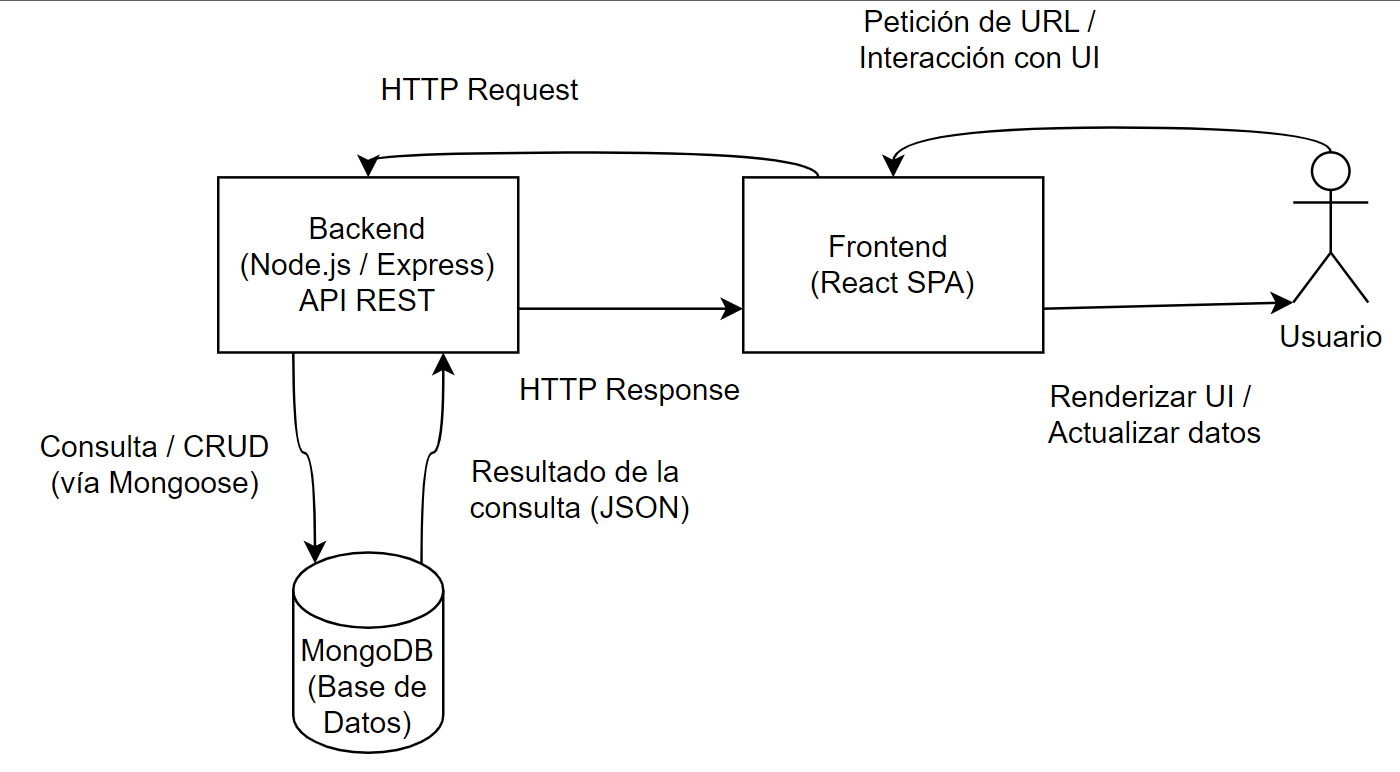
\includegraphics[clip=true,width=\textwidth]{img/arquitectura_logica_logart.png}\\

    \footnotesize (a)
  \end{minipage}
  \caption{Diagrama de Arquitectura Lógica de Alto Nivel de LogArt.}\label{fig:arquitecturaLogica}
  \end{figure}

\subsection{Arquitectura de Despliegue (Simplificada)}
\label{ssec:arquitecturaDespliegue}

La arquitectura lógica descrita anteriormente se implementa y despliega utilizando tecnología de contenerización, específicamente Docker y Docker Compose (ver Sección: \ref{sec:contenedores}). Este enfoque asegura la portabilidad, consistencia y facilidad de gestión del entorno de la aplicación, tanto para desarrollo como para una eventual puesta en producción.

Los componentes principales de la aplicación LogArt se empaquetan en contenedores Docker, la orquestación de estos contenedores se gestiona mediante Docker Compose.

La arquitectura de despliegue de LogArt se compone de los siguientes servicios principales definidos en el archivo \texttt{docker-compose.yml}

\begin{itemize}
    \item \textbf{Servicio \texttt{app} (Contenedor de la Aplicación LogArt):}
    \begin{itemize}
        \item Este contenedor ejecuta la aplicación backend Node.js/Express.js.
        \item También es responsable de servir los archivos estáticos del frontend React, que son compilados y copiados a una carpeta pública dentro de este contenedor durante el proceso de construcción de la imagen Docker (como se detalló en la Sección \ref{sec:contenedores} sobre el \texttt{Dockerfile} multi-etapa).
        \item Se expone un puerto para permitir el acceso a la aplicación desde el exterior del contenedor, utilizando HTTPS con certificados auto firmados para el entorno de desarrollo.
        \item La configuración específica del entorno (como credenciales de base de datos, secretos de API, etc) se gestiona mediante variables de entorno, cargadas a través de un archivo \texttt{.env}.
    \end{itemize}
    \item \textbf{Servicio \texttt{mongo} (Contenedor de la Base de Datos MongoDB):}
    \begin{itemize}
        \item Este contenedor ejecuta una instancia de la base de datos MongoDB.
        \item Utiliza una imagen oficial de MongoDB proveniente de DockerHub.
        \item La base de datos es accesible para el servicio \texttt{app} a través de una red interna definida por Docker Compose.
    \end{itemize}
\end{itemize}

Ambos servicios (\texttt{app} y \texttt{mongo}) están configurados con \textit{healthchecks} en el archivo \texttt{docker-compose.yml} para monitorizar su estado y gestionar dependencias de arranque, asegurando que, por ejemplo, la aplicación no intente conectarse a la base de datos antes de que esta esté completamente operativa.

\begin{figure}
   \centering

  \begin{minipage}{0.45\textwidth}
   \centering

     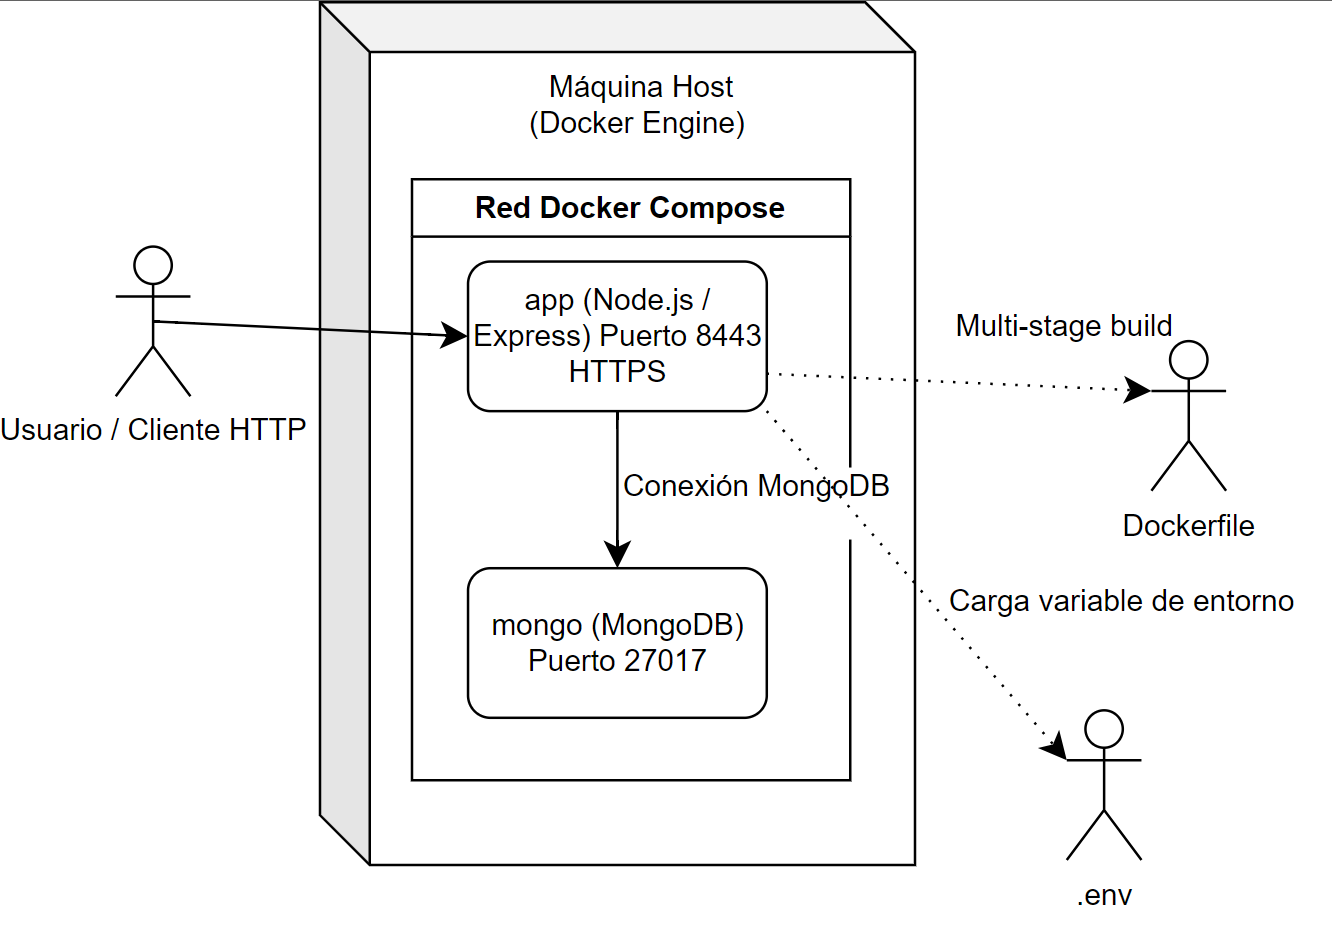
\includegraphics[clip=true,width=\textwidth]{img/arquitectura_despliegue_logart.png}\\

    \footnotesize (b)
  \end{minipage}
  \caption{Diagrama de Arquitectura de Despliegue Simplificado de LogArt.}\label{fig:arquitecturaDespliegue}
  \end{figure}

Esta arquitectura de despliegue basada en contenedores no solo facilita el entorno de desarrollo local, sino que también sienta las bases para despliegues más robustos en entornos de producción, ya que las mismas imágenes y configuraciones de Docker Compose pueden ser utilizadas en plataformas que soporten contenedores

\subsection{Diseño del Backend}
\label{ssec:disenoBackend}

El backend de LogArt, desarrollado con Node.js y el framework Express.js, ha sido estructurado siguiendo principios de modularidad y separación de responsabilidades para facilitar su desarrollo, mantenimiento y comprensión. A continuación, se describe su organización interna y el modelo de datos subyacente.

\subsubsection{Estructura de Directorios y Organización del Código}
\label{sssec:estructuraBackend}

El código fuente del backend de LogArt se organiza en una estructura de directorios que refleja una separación clara de las diferentes funcionalidades y capas de la aplicación. La estructura principal, ubicada dentro de la carpeta \texttt{LogArtApp/backend/}, es la siguiente (se omiten archivos de configuración o irrelevantes para centrarse en los directorios de lógica):

\begin{itemize}
    \item \textbf{\texttt{/config}:} Contiene archivos de configuración de la aplicación, como la configuración de la conexión a la base de datos, o la gestión de claves SSL para HTTPS.
    \item \textbf{\texttt{/controllers}:} Alberga los controladores de la aplicación. Cada controlador es responsable de manejar las peticiones HTTP entrantes para un recurso específico (ej. \texttt{userController.js}, \texttt{objectController.js}), validar los datos de entrada (requiriendo ayuda de middlewares y servicios de validación), invocar la lógica de negocio apropiada en los servicios, y formular la respuesta HTTP que se enviará al cliente.
    \item \textbf{\texttt{/middlewares}:} Contiene funciones middleware personalizadas que se utilizan en el flujo de procesamiento de peticiones Express.js. Por ejemplo, middleware para la autenticación y autorización de usuarios (verificando tokens JWT), manejo de subida de imágenes, o verificación de roles.
    \item \textbf{\texttt{/models}:} Define los esquemas y modelos de datos utilizando Mongoose. Cada archivo en este directorio (ej. \texttt{user.model.js}, \texttt{object.model.js}, \texttt{comment.model.js} describe la estructura de los documentos que se almacenarán en las colecciones de MongoDB, incluyendo los tipos de datos, validaciones, valores por defecto, índices y relaciones.
    \item \textbf{\texttt{/repositories}:} Esta capa, abstrae las interacciones directas con los modelos Mongoose, proporcionando una interfaz más genérica para el acceso a datos. Los servicios invocan a los repositorios en lugar de a los modelos directamente.
    \item \textbf{\texttt{/routes}:} Contiene los archivos que definen las rutas de la API RESTful. Cada archivo de ruta (ej. \texttt{/userRoutes.js}, \texttt{/objectRoutes.js}) agrupa los endpoints relacionados con un recurso específico y los asocia con las funciones controladoras correspondientes. Estos archivos son luego montados en la aplicación principal de Express.
    \item \textbf{\texttt{/Seeders}:} Incluye scripts para poblar la base de datos con datos iniciales de prueba (ej. usuarios administradores, disciplinas iniciales, datos de ejemplo para desarrollo). Estos scripts son útiles para configurar el entorno de desarrollo rápidamente.
    \item \textbf{\texttt{/services}:} Esta capa contiene la lógica de negocio principal de la aplicación. Los servicios son invocados por los controladores y son responsables de orquestar las operaciones, aplicar reglas de negocio, y interactuar con los repositorios para acceder y manipular los datos.
    \item \textbf{\texttt{/utils}:} Directorio para funciones de utilidad o helpers re utilizables, como el envío de correos, la validación de un id según MongoDB, o la función \texttt{notifyAdmins} con sockets.
    \item \textbf{\texttt{/\textunderscore \textunderscore test\textunderscore\textunderscore}:} Contiene los archivos de pruebas automatizadas para el backend, utilizando Jest y Supertest. \ref{sec:herramientasPruebas}
    \item \textbf{\texttt{/api-docs}:} Almacena la especificación OpenAPI (Swagger) generada para la documentación de la API.
\end{itemize}
Los archivos principales en la raíz del backend, como \texttt{app.js} (o \texttt{server.js}), se encargan de configurar e inicializar la aplicación Express, montar las rutas, aplicar middlewares globales e iniciar el servidor. Esta estructura modular facilita la navegación por el código, la adición de nuevas funcionalidades y el mantenimiento del sistema.

En la figura \ref{fig:diagramaClasesBackend} se muestra el diagrama de clases del backend.

\begin{figure}
   \centering

  \begin{minipage}{0.45\textwidth}
   \centering

     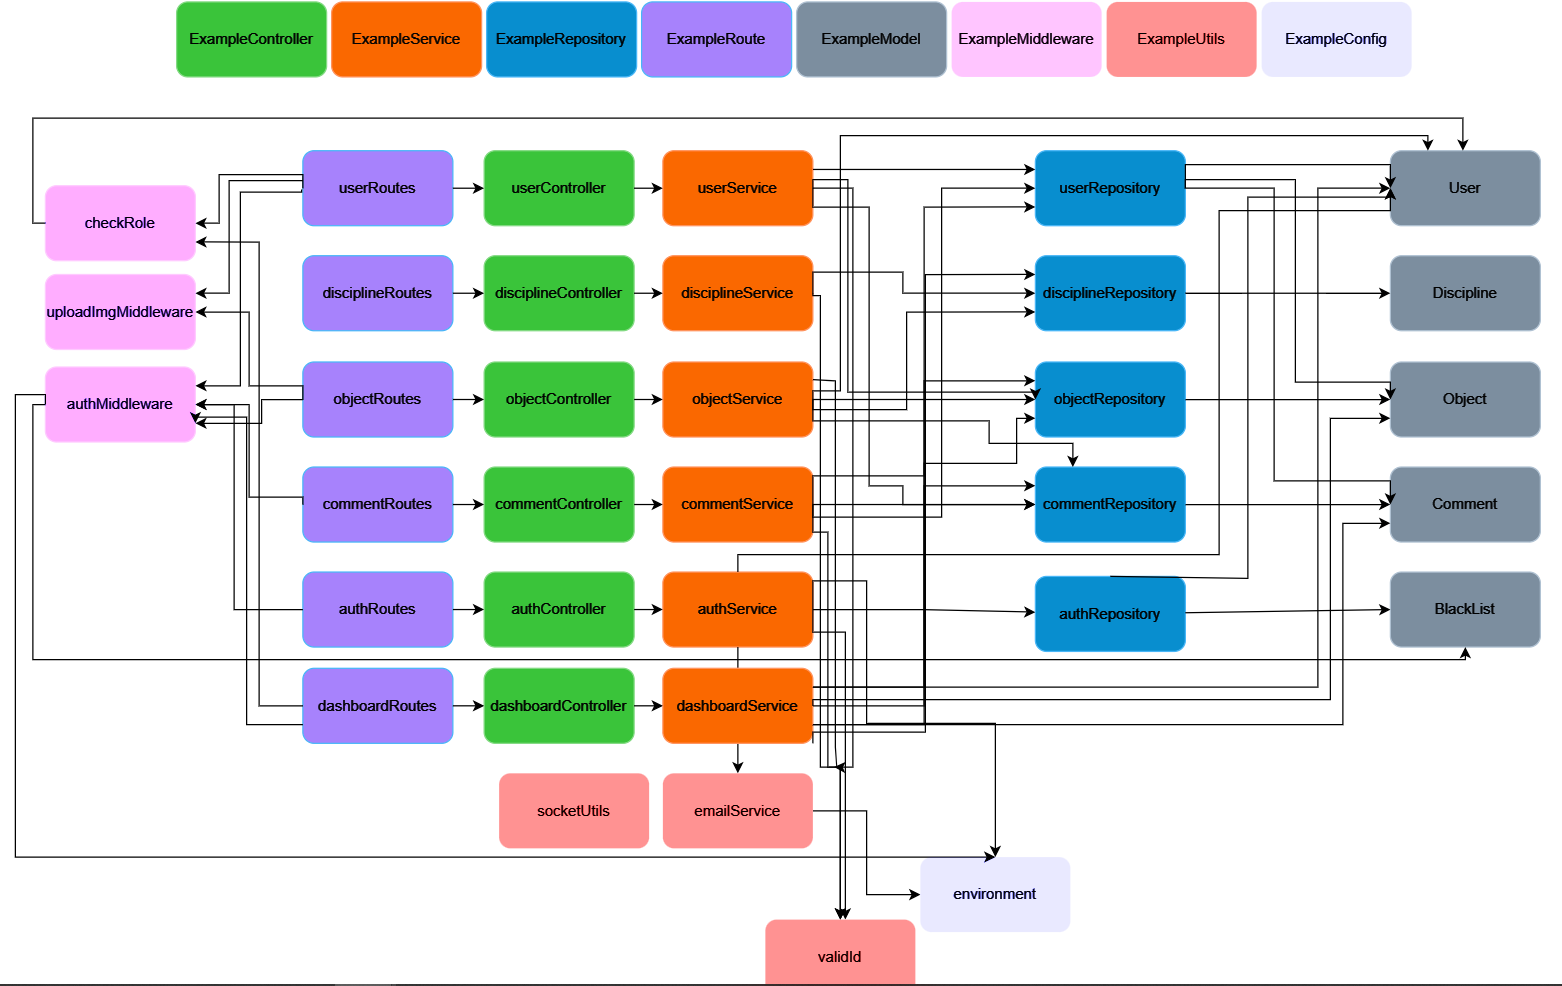
\includegraphics[clip=true,width=\textwidth]{img/diagrama_clases_backend_logart.png}\\

    \footnotesize (c)
  \end{minipage}
  \caption{Diagrama de Clases del Backend de la Aplicación.}\label{fig:diagramaClasesBackend}
  \end{figure}

\subsubsection{Modelo de Dominio y Diagrama de Clases del Backend}
\label{sssec:modeloDominioBackend}

El modelo de dominio del backend representa las entidades principales de LogArt y sus interrelaciones. Estas entidades se corresponden directamente con los modelos definidos mediante Mongoose y las colecciones en la base de datos MongoDB. Las entidades clave son:
\begin{itemize}
    \item \textbf{User (Usuario):} Representa a un usuario de la aplicación, con atributos como nombre de usuario, correo, contraseña (hasheada), nombre, apellidos, biografía, imagen de perfil, rol, entre otros.
    \item \textbf{Object (Objecto):} Representa una entrada de una obra creada por un usuario, asociada a una disciplina. Contiene atributos como título, descripción, imagen, fecha de creación, referencia al usuario propietario, y un indicador de si está compartido o no.
    \item \textbf{Comment (Comentario):} Representa una anotación o recuerdo detallado asociado a un \texttt{Object}. Contiene el texto del comentario, la fecha de creación, si ha sido por un admin o no, y el id del objeto al que pertenece.
    \item \textbf{Discipline (Disciplina):} Representa las categorías principales de la web, como ``Libros'', ``Canciones'' y ``Videojuegos''. Contiene simplemente el nombre de la entidad y la descripción.
    \item \textbf{BlackListedToken:} Representa un token en la lista negra, contiene el token y la fecha de caducidad, en la que será borrado automáticamente de la base de datos.
\end{itemize}

Las relaciones principales entre estas entidades son:
\begin{itemize}
    \item Un \texttt{User} puede crear muchos \texttt{Object's} (relación uno a muchos).
    \item Un \texttt{Object} pertenece a un solo \texttt{User} (propietario).
    \item Un \texttt{Object} puede tener muchos \texttt{Comment's} (relación uno a muchos).
    \item Un \texttt{Comment} pertenece a un solo \texttt{Object} y es creado por un \texttt{user}.
    \item Un \texttt{Object} está asociado a una \texttt{Discipline}.
    \item \texttt{BlackListToken} representa un token que ha sido invalidado por alguna razón, y por tanto, ha entrado en la lista negra.
\end{itemize}

En la figura \ref{fig:diagramaEntidadesBD} se  representa el diagrama de entidades de la base de datos, que ilustra estas entidades y sus relaciones. Mientras que en el \ref{fig:diagramaEntidadesBDSimple} se muestra a un nivel más alto de abstracción.

\begin{figure}
   \centering

  \begin{minipage}{0.45\textwidth}
   \centering

     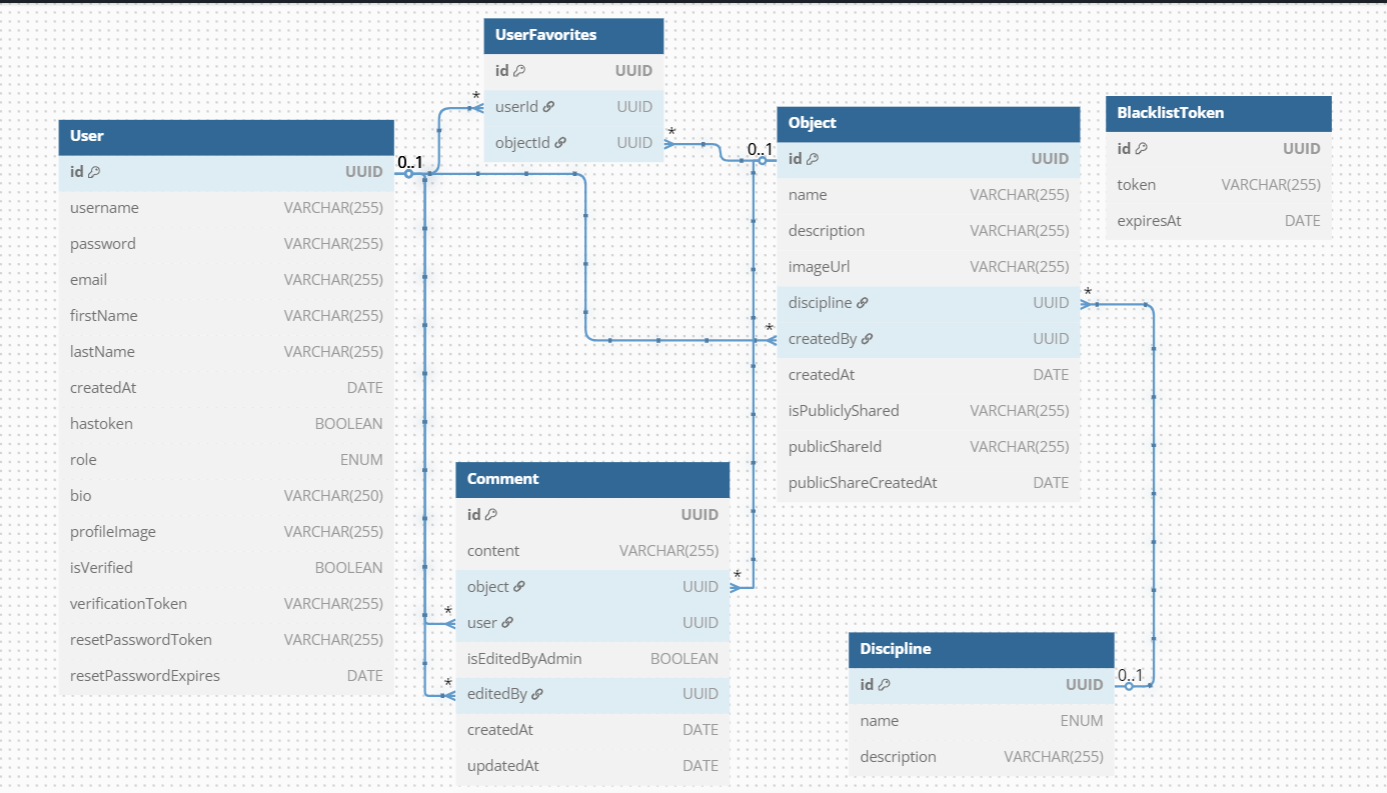
\includegraphics[clip=true,width=\textwidth]{img/diagrama_entidades_basedatos.png}\\

    \footnotesize (d)
  \end{minipage}
  \caption{Diagrama de Entidades de la Base de Datos.}\label{fig:diagramaEntidadesBD}
  \end{figure}

\begin{figure}
   \centering

  \begin{minipage}{0.45\textwidth}
   \centering

     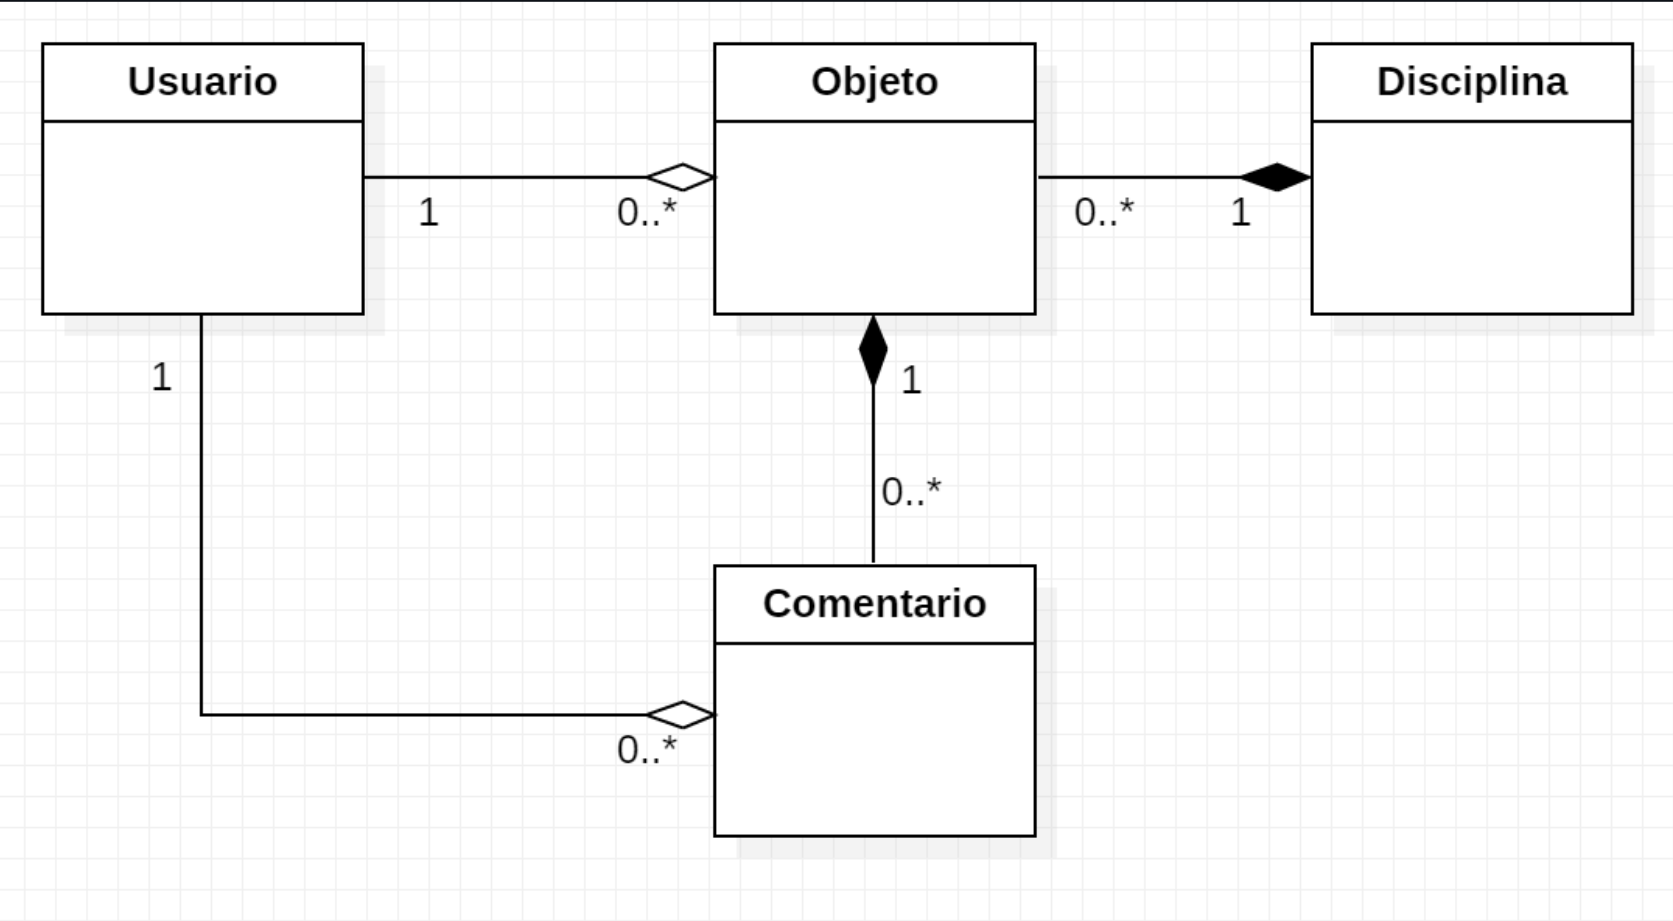
\includegraphics[clip=true,width=\textwidth]{img/diagrama_entidades_altonivel.png}\\

    \footnotesize (d.2)
  \end{minipage}
  \caption{Diagrama de Entidades de la Base de Datos, con mayor nivel de abstracción.}\label{fig:diagramaEntidadesBDSimple}
  \end{figure}

\subsection{Diseño del Frontend (Single Page Application)}
\label{ssec:disenoFrontend}

El frontend de LogArt se ha desarrollado como una Single Page Application (SPA) utilizando la biblioteca/framework React. Este enfoque permite una experiencia de usuario fluida y dinámica, donde las transiciones entre diferentes vistas y la actualización de contenido se realizan sin necesidad de recargar la página completa desde el servidor. La estructura y los componentes principales del frontend se describen a continuación.

\subsubsection{Estructura de Directorios y Organización de Componentes}
\label{sssec:estructuraFrontend}

El código fuente de LogArt, ubicado en la carpeta \texttt{/LogArt-frontend/}, se organiza para promover la modularidad y la reutilización de componentes. La estructura principal dentro del directorio \texttt{src/} es la siguiente:
\begin{itemize}
    \item \textbf{\texttt{/components}:} Este directorio contiene componentes de React reutilizables que se utilizan en diversas partes de la aplicación. Entre estos se incluyen componentes de UI genéricos (ej. botones, modales, tarjetas de objetos) o componentes más específicos que encapsulan la porción de la interfaz y su lógica. El objetivo es fomentar la composición y evitar la duplicación de código. Algunos ejemplos claves son:
    \begin{itemize}
        \item \texttt{CommentList.jsx}
        \item \texttt{DisciplineSelector.jsx}
        \item \texttt{Navbar.jsx}
        \item \texttt{ObjectCard.jsx}.
    \end{itemize} 
    \item \textbf{\texttt{/context}:} Aquí se definen los Contextos de React. La API de contexto de React se utiliza para gestionar el estado global o compartido entre componentes que no están directamente relacionados en el árbol de componentes.
    \begin{itemize}
        \item \texttt{AuthContext}: Gestiona el estado de autenticación del usuario (si está logueado, datos del usuario, token JWT) y proporciona funciones para iniciar y cerrar sesión.
        \item \texttt{ModalContext}: Controla la visibilidad y el contenido de los modales genéricos utilizados en la aplicación
        \item \texttt{SocketContext}: Administra la conexión y los eventos de WebSockets (Socket.IO) para funcionalidades en tiempo real, como las notificaciones del administrador.
    \end{itemize}
    \item \textbf{\texttt{/pages}:} Contiene los componentes de React que representan las diferentes ``páginas'' o vistas principales de la aplicación (ej. \texttt{Hero.jsx}, \texttt{ObjectDetail.jsx}, \texttt{Profile.jsx}). Estos componentes se componen de varios componentes más pequeños del directorio \texttt{/components} y gestionan la lógica específica de cada vista.
    \item \textbf{\texttt{/utilities}:} Directorio para funciones o archivos de utilidad, como \texttt{api.js} que centraliza las llamadas a la API con Axios, o \texttt{faqs.jsx}, que contiene las preguntas y respuestas que se mostrarán en la página inicial.
    \item \textbf{\texttt{App.jsx}:} Es el componente raíz de la aplicación React. Se encarga de configurar el enrutador (React Router DOM) y de renderizar los componentes de página según la ruta actual.
    \item \textbf{\texttt{main.jsx}:} Es el punto de entrada de la aplicación React, donde se renderiza el componente \texttt{App.jsx}.
    \item \textbf{\texttt{/ui-test/tests}:} Directorio que alberga las pruebas End-to-End implementadas con Playwright para validar la interfaz de usuario y los flujos de interacción.
\end{itemize}

Esta organización busca mantener el código ordenado, facilitando la localización de componentes y la facilidad de desarrollo.

En la Figura \ref{fig:diagramaComponentesFrontend} se presenta un diagrama que ilustra la relación entre: componentes, páginas, contexto y utilidad, mostrando como se componen para formar las diferentes vistas que el usuario experimenta. El diagrama se enfoca en la estructura y las relaciones entre componentes, más que en el flujo de datos detallado, para ofrecer una visión general de la arquitectura de la SPA.

\begin{figure}
   \centering

  \begin{minipage}{0.45\textwidth}
   \centering

     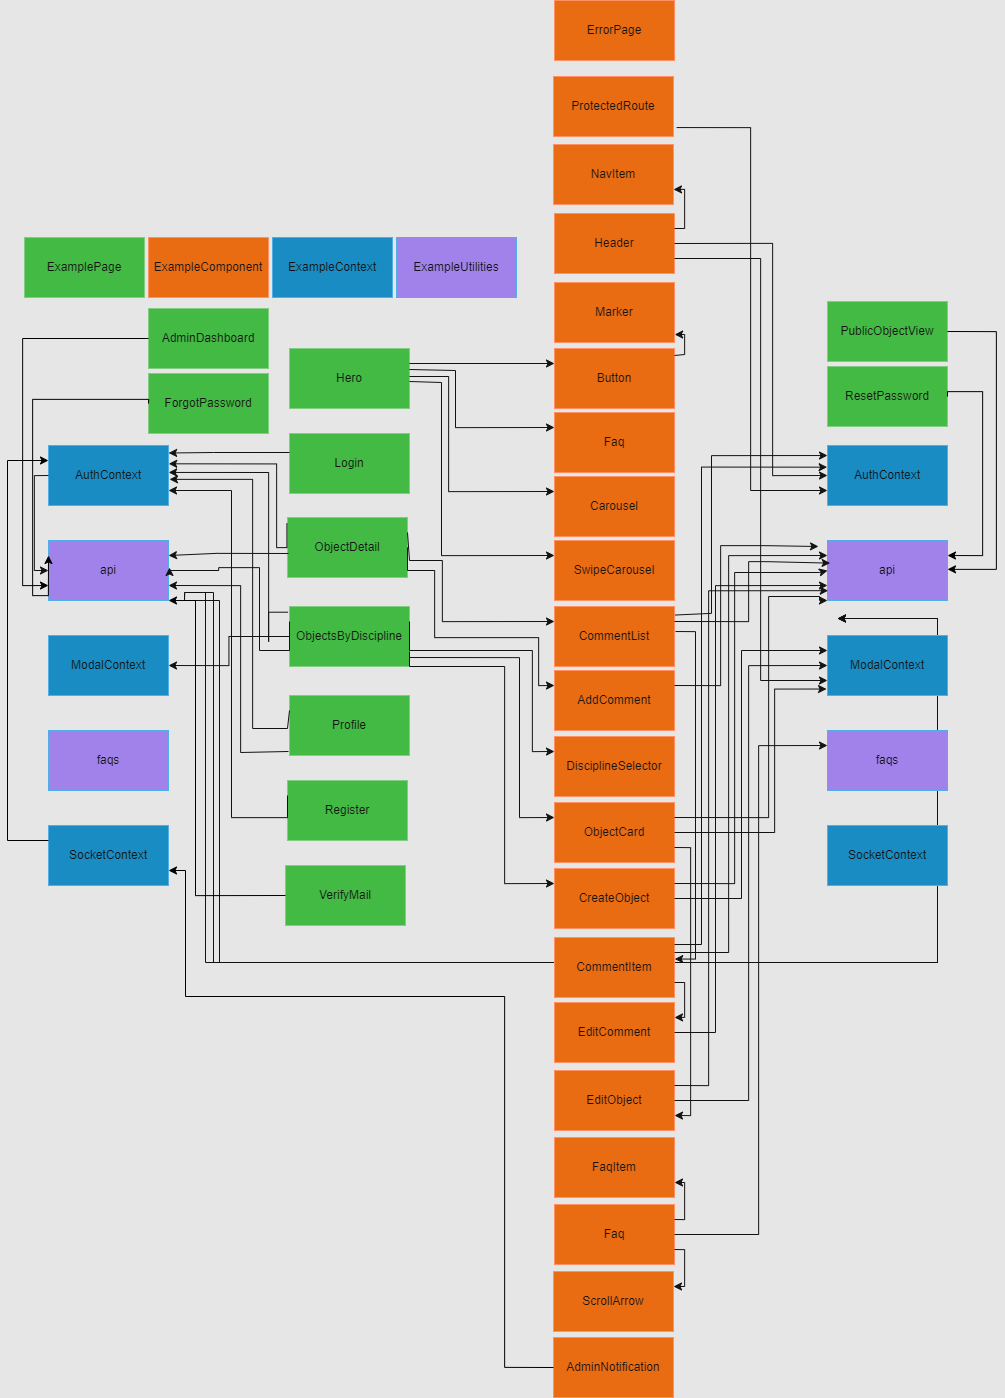
\includegraphics[clip=true,width=\textwidth]{img/diagrama_componentes_frontend_logart.png}\\

    \footnotesize (e)
  \end{minipage}
  \caption{Diagrama de Componentes Frontend de la aplicación.}\label{fig:diagramaComponentesFrontend}
  \end{figure}

\section{Diseño e Implementación}
\label{sec:disenoImplementacion}

Tras la descripción de la arquitectura general de LogArt en la sección anterior, este apartado se adentra en los detalles concretos del diseño interno y la implementación de sus componentes y funcionalidades clave. El objetivo es ofrecer una visión más profunda de cómo se han traducido los requisitos y las decisiones arquitectónicas en código funcional, destacando las soluciones técnicas adoptadas, y algunos de los aspectos más relevantes del proceso de desarrollo.

Se explorarán tanto el diseño del backend, centrándose en la estructura de su API RESTful y la integración con la base de datos, como el diseño frontend, detallando la gestión del estado y la composición de la interfaz de usuario en React. Además, se abordarán aspectos específicos de la implementación, como la resolución de desafíos técnicos particulares o la descripción de una funcionalidad destacada del sistema. 

Este análisis detallado busca no solo documentar la aplicación construida, sino también justificar las decisiones e implementación tomadas, proporcionando al lector una comprensión clara de la ingeniería detrás de LogArt.

\subsection{Diseño e Implementación del Backend}
\label{ssec:disenoImplBackend}

El backend de LogArt, construido sobre Node.js y Express.js, es el responsable de la lógica de negocio, la gestión de datos y la exposición de una API RESTful. Su diseño se ha centrado en la modularidad, la separación de responsabilidades y la seguridad.

\subsubsection{API RESTful: Diseño y Flujo de Peticiones}
\label{sssec:apiRestfulDiseno}

La comunicación entre el frontend y el backend se realiza a través de una API RESTful. Se han seguido los principios estándar de diseño REST, como el uso de métodos HTTP semánticos (GET, POST, PUT, DELETE), la representación de recursos a través de URLs claras y el uso de códigos de estado HTTP para indicar el resultado de las operaciones. Todas las respuestas de la API se devuelven en formato JSON.

La estructura de las rutas de la API, definidas en el directorio \texttt{/routes} ( por ejemplo \texttt{objectRoutes.js}, sigue un patrón basado en recursos. Por ejemplo, todas las operaciones relacionadas con los ``objetos'' se agrupan bajo el prefijo \texttt{/api/v1/objects}. El archivo \texttt{app.js} centraliza la configuración de la aplicación Express, incluyendo el montaje de estas rutas y la aplicación de middlewares globales como \texttt{cors} (para la gestión de Intercambio de Recursos de Origen Cruzado) y \texttt{express.json()} (para el parseo de cuerpos de petición JSON).

El flujo típico de una petición a un endpoint protegido es el siguiente:
\begin{enumerate}
    \item El cliente (frontend), a través de alguna acción en la interfaz, realiza una petición HTTP a un endpoint de la API, incluyendo un JSON Web Token (JWT) en la cabecera \texttt{Authorization} (ej. \texttt{Bearer token}).
    \item La petición llega a la aplicación Express.js
    \item El middleware de autenticación (\texttt{verifyToken} en \texttt{authMiddleware.js})  intercepta la petición. Este middleware:
    \begin{itemize}
        \item Verifica la presencia y validez del token JWT.
        \item Comprueba si el token está en una lista negra (modelo \texttt{BlaclistedToken}) para tokens revocados (ej. tras un cierre de sesión).
        \item Si el token es válido y no está en la lista negra, decodifica el payload del usuario (que incluye \texttt{userId} y \texttt{role}) y los adjunta al objeto \texttt{req} (ej. \texttt{req.user}).
        \item Si el token es inválido o no se proporciona, se devuelve una respuesta de error (401 no Autorizado o 403 Prohibido).
    \end{itemize}
    \item Si la autenticación es exitosa, la petición pasa al siguiente punto de la validación.
    \item El controlador extrae los datos necesarios de la petición (\texttt{req.params}, \texttt{req.body}, \texttt{req.query} y \texttt{req.file} para subida de archivos con \texttt{multer}, como se puede ver en \texttt{objectRoutes.js} para la creación y actualización de objetos).
    \item El controlador invoca la función apropiada en el módulo de servicio correspondiente (ej. \texttt{objectService.js}), pasándole los datos validados y el \texttt{userId} del usuario autenticado.
    \item El servicio aplica la lógica de negocio, interactuando con los repositorios (ej. \texttt{objectRepository.js}) que a su vez operan sobre los modelos Mongoose (ej. \texttt{object.model.js}) para realizar las operaciones CRUD en la base de datos MongoDB.
    \item El servicio devuelve el resultado (o un error) al controlador.
    \item El controlador construye la respuesta HTTP (Código de estado, cabeceras como \texttt{Location} para creaciones exitosas, y cuerpo JSON) y la envía de vuelta al cliente.
\end{enumerate}

Un ejemplo de este flujo se puede observar en la creación de un objeto (controlador \texttt{createObject} en \texttt{objectController.js}): 
\begin{itemize}
    \item La ruta \texttt{POST /api/v1/objects} está protegida por \texttt{verifyToken} y utiliza el middleware \texttt{uploadObject.single(``imageUrl'')} para manejar la subida de la imagen.
    \item El controlador luego llama a \texttt{objectService.createObject}, que valida los datos, interactúa con \texttt{disciplineRepository} y \texttt{objectRepository}, y finalmente devuelve el objeto creado o un error.
    \item El controlador entonces responde al cliente con un estado 201 y la ubicación del nuevo recurso.
     
\end{itemize}   
La documentación de la API, generada con Swagger a partir de anotaciones JSDoc en los controladores, detalla todos los endpoints disponibles, sus parámetros y esquemas de respuesta.

\subsubsection{Interacción con la Base de Datos y Lógica de Negocio}
\label{sssec:backendDbLogica}

La persistencia de datos se gestiona a través de MongoDB, con una capa de abstracción proporcionada por Mongoose. Los modelos (ej. \texttt{object.model.js}) definen la estructura de los datos, incluyendo tipos, campos requeridos, valores por defecto, relaciones mediante \texttt{Schema.Types.ObjectId} y la propiedad \texttt{ref}.

Los \textbf{repositorios} (ej. \texttt{objectRepository.js}) encapsulan las consultas directas a la base de datos utilizando los modelos Mongoose. Proporcionan métodos específicos para las operaciones CRUD y consultas más complejas (ej. \texttt{findObjects} con filtros, paginación y populación de campos referenciados; \texttt{findByPublicShareId}). Esta capa de repositorio ayuda a desacoplar la lógica de negocio de los detalles de implementación de Mongoose.

Los \textbf{servicios} (ej. \texttt{objectService.js} contienen la lógica de negocio principal. Por ejemplo, el servicio \texttt{objectService}:
\begin{itemize}
    \item Valida la existencia de disciplinas antes de crear o actualizar un objeto.
    \item Verifica los permisos del usuario para actualizar o eliminar un objeto, permitiendo estas acciones solo al propietario o a un administrador.
    \item Gestiona la eliminación de imagen asociadas cuando un objeto se actualiza o elimina (evitando dejar archivos huérfanos, con la excepción de las imágenes por defecto).
    \item Maneja la lógica para compartir públicamente un objeto, generando un id único (\texttt{publicShareId}) y gestionando su estado \texttt{isPubliclyShared}.
    \item En la función \texttt{togglePublicShare}, interactúa con \texttt{socketUtils} para notificar a los administradores cuando un objeto se comparte, demostrando la integración con WebSockets.
\end{itemize}

En resumen, el diseño del backend de LogArt se ha organizado de forma modular para garantizar la separación de responsabilidades entre rutas, controladores, servicios y repositorios. Gracias al uso de middleware para autenticación, la lógica de validación y la de gestión de errores, así como a la abstracción de la persistencia mediante Mongoose, conseguimos un API RESTful robusto, seguro y fácil de mantener. Además, la integración con Swagger facilita la generación ``Automática'' de la documentación.

A continuación, en la Sección \ref{ssec:disenoImplFrontend}, abordaremos el diseño e implementación del frontend en React, donde veremos cómo esta capa consume la API, maneja el estado de la aplicación y construye la interfaz de usuario en LogArt.

\subsection{Diseño e Implementación del Frontend (React)}
\label{ssec:disenoImplFrontend}

El frontend de LogArt, desarrollado como un Single Page Application (SPA) con React, es el punto de interacción directo con el usuario. Su diseño se ha enfocado en la creación de una interfaz intuitiva, responsiva y modular, utilizando componentes reutilizables y una gestión de estado eficiente.

\subsubsection{Gestión de Estado con Context API}
\label{sssec:frontendEstadoContext}

Para gestionar el estado global o compartido a través de diferentes componentes de la aplicación se ha utilizado la API de contexto de React. Los principales contextos implementados son:

\begin{itemize}
    \item \textbf{\texttt{AuthContext.jsx}:} Este contexto es fundamental para la gestión de la autenticación del usuario.
    \begin{itemize}
        \item Mantiene el estado del usuario actual (\texttt{user}), un booleano \texttt{isAuthenticated} que indica si el usuario ha iniciado sesión, y un estado de carga \texttt{loading} para gestionar la verificación inicial del token.
        \item Almacena el token JWT el \texttt{localStorage} tras un inicio de sesión exitoso y lo configura en las cabeceras por defecto de Axios (ver \texttt{utilities/api.jsx}).
        \item Intenta cargar el perfil del usuario al iniciarse la aplicación si existe un token en \texttt{localStorage}, manteniendo así la sesión del usuario entre recargas.
        \item Proporciona funciones para \texttt{login}, \texttt{register}, \texttt{logout}, que encapsulan las llamadas a la API del backend y actualizan el estado de autenticación en consecuencia. La función \texttt{logout} también se encarga de eliminar el token de \texttt{localStorage} y de la lista negra del backend.
    \end{itemize}
    \item \textbf{\texttt{ModalContext.jsx}:} Proporciona una forma centralizada de gestionar la apertura y cierre de componentes modales genéricos en toda la aplicación.
    \begin{itemize}
        \item Mantiene el estado del modal actualmente visible (\texttt{currentModal}) y sus propiedades (\texttt{modalProps}).
        \item Ofrece funciones \texttt{openModal} (que recibe el componente modal a renderizar y sus props) y \texttt{closeModal}.
        \item Incluye un efecto (\texttt{useEffect}) para deshabilitar el scroll del cuerpo de la página cuando un modal está activo, mejorando la experiencia de usuario. El componente modal se renderiza directamente desde el proveedor del contexto.
    \end{itemize}
    \item \textbf{\texttt{SocketContext.jsx}:} Gestiona la conexión y los eventos de WebSockets para funcionalidades en tiempo real. Este contexto encapsula la lógica de conexión al servidor de sockets y la suscripción/emisión de eventos.
\end{itemize}

Además del estado global gestionado por Context, los componentes individuales utilizan el estado local (\texttt{useState}, \texttt{useEffect}) para manejar su propia lógica de UI y datos temporales.

\subsubsection{Flujo de Datos y Comunicación con la API}
\label{sssec:frontendFlujoDatosApi}

La interacción con la API RESTful del backend se centraliza principalmente a través de una instancia de Axios configurada en \texttt{utilities/api.jsx}. Esta instancia define la \texttt{baseURL} del servidor backend (\texttt{https://localhost:8443}) y utiliza interceptores de petición para adjuntar automáticamente el token JWT (obtenido de \texttt{localStorage} a través del \texttt{AuthContext}) a la cabecera \texttt{Authorization} de cada solicitud, simplificando las llamadas a endpoints protegidos.

Los componentes de página (ubicados en \texttt{/pages}), como \texttt{ObjectsByDiscipline.jsx}, son generalmente responsables de:
\begin{itemize}
    \item Obtener los datos necesarios para su vista al montarse (utilizando \texttt{useEffect} y funciones asíncronas que llaman al servicio \texttt{api}).
    \item Manejar la lógica de paginación, búsqueda (con debounce como se puede ve en \texttt{ObjectsByDiscipline.jsx} para optimizar las peticiones mientras el usuario escribe) y filtrado (ej. ``mostrar solo favoritos'').
    \item Pasar los datos y funciones de callback necesarias a los componentes de prestación hijos.
    \item Actualizar su estado local (y, por ende, la UI) en respuesta a las acciones del usuario o a los datos recibidos de la API.
\end{itemize}
El componente \texttt{App.jsx} actúa como el orquestador principal del frontend, configurando el enrutador \texttt{react-router-dom} para mapear las URLs a los componentes de página correspondientes. Utiliza el componente \texttt{ProtectedRoute} para restringir el acceso a ciertas rutas basándose en el estado de autenticación del usuario y, opcionalmente, en su rol (ej. para el \texttt{/admin/dashboard}).

\subsubsection{Componentes Reutilizables Clave}
\label{sssec:frontendComponentesReutilizables}

La modularidad del frontend se logra mediante el uso extensivo de componentes reutilizables, algunos ejemplos destacados son:
\begin{itemize}
    \item \textbf{\texttt{Header.jsx}: } Componente estructural presente en la mayoría de las vistas, proporcionando navegación principal y enlaces comunes.
    \item \textbf{\texttt{DisciplineSelector.jsx}:} Un componente de UI que permite al usuario seleccionar una disciplina de una lista desplegable. Gestiona su propio estado de apertura y maneja la selección del usuario, notificando al componente padre del cambio.
    \item \textbf{\texttt{ObjectCard.jsx}:} Representa la vista en miniatura de un objeto en la galería. Muestra información clave del objeto (imagen, nombre, descripción breve, creador) y proporciona acciones como editar, eliminar (si el usuario es el propietario) y marcar/desmarcar como favorito. Este componente encapsula la lógica para estas acciones, incluyendo las llamadas a la API y la actualización del estado local o global (a través de callbacks o contexto).
    \item \textbf{\texttt{CreateObject.jsx} y \texttt{(EditObject.jsx}):} Componentes modales (gestionados por \texttt{ModalContext}) que presentan formularios para la creación y edición de objetos. Manejan el estado del formulario, la validación de entrada, la subida de imágenes (\texttt{multipart/form-data}) y la comunicación con la API para persistir los cambios.
    \item \textbf{\texttt{ProtectedRoute.jsx}:} Un componente de orden superior que envuelve rutas para restringir el acceso solo a usuarios autenticados y, opcionalmente, a roles específicos (ej. \texttt{admin}). Redirige a la página de inicio de sesión si no se cumplen las condiciones.
\end{itemize}

Estos componentes, entre muchos otros, permiten construir interfaces complejas de forma eficiente y mantener una base de código organizada.

\subsection{Foco en una Parte del Desarrollo: El Panel de Administración}
\label{ssec:focoAdminDashboard}

Una de las funcionalidades avanzadas y más complejas implementadas en LogArt es el Panel de Administración o Admin Dashboard. Esta sección está diseñada para proveer al rol de Administrador una visión general del estado de la plataforma, estadísticas detalladas sobre usuarios y contenido, y herramientas para la moderación. A continuación, se detalla su diseño e implementación tanto en el backend como en el frontend.
\paragraph{Requisitos Específicos del Admin Dashboard:}
El dashboard debía cumplir con los siguientes requisitos funcionales principales (derivados de RF6 en la Sección \ref{rf:adminFuncionalidades}):
\begin{itemize}
    \item Presentar un resumen general (overview) con métricas clave (total de usuarios, objetos, comentarios).
    \item Ofrecer estadísticas detalladas sobre los usuarios (distribución por rol, usuarios más activos).
    \item Proporcionar un análisis del contenido (distribución de objetos por disciplina, objetos más comentados).
    \item Mostrar la actividad de creación de contenido a lo largo del tiempo (semanal, mensual, trimestral).
    \item Analizar el crecimiento de usuarios, objetos y comentarios comparando periodos.
    \item Permitir la visualización y moderación (eliminación) de todos los objetos y usuarios de la plataforma.
    \item Ser accesible únicamente por usuarios con el rol de ``admin''.
\end{itemize}

\paragraph{Diseño e Implementación en el Backend:}El backend expone una serie de endpoints específicos bajo la ruta \texttt{/api/v1/dashboard/}, todos protegidos para ser accesibles únicamente por administradores mediante el middleware \texttt{authMiddleware.js}
\begin{itemize}
    \item \textbf{Rutas y Controladores:} El archivo \texttt{dashboardRoutes.js} define las rutas para cada sección del dashboard (ej. \texttt{/overview} , \texttt{/activity, etc}). Cada ruta está asociada a una función en \texttt{dashboardController.js}, que actúa como intermediario, recibiendo la petición y llamando al servicio correspondiente.
    \item \textbf{Servicio del Dashboard (\texttt{dashboardService.js}):} Este servicio es el corazón de la lógica del dashboard en el backend. Contiene funciones que realizan agregaciones complejas y consultas a la base de datos MongoDB utilizando los modelos Mongoose (a través de los repositorios) para recopilar y procesar los datos necesario para cada estadística. Destacan las siguientes funcionalidades:
    \begin{itemize}
        \item \textbf{Agregaciones con MongoDB Aggregate Framework:} Para muchas estadísticas, como \texttt{objectsByDiscipline}, \texttt{usersByRole}, \texttt{usersByObjectCount}, y \texttt{mostCommentedObjects}, se utiliza el potente \textit{Aggregation Framework} de MongoDB. Por ejemplo, para \texttt{objectsByDiscipline}, se realiza un \texttt{\$lookup} para unir con la colección de disciplinas y luego un \texttt{\$group} para contar objetos por nombre de disciplina.
        \item \textbf{Cálculo de Crecimiento:} La función \texttt{getGrowthAnalysis} calcula el porcentaje de crecimiento para usuarios, objetos y comentarios comparando el periodo actual (semanal, mensual, trimestral) con el periodo inmediatamente anterior. Utiliza una función auxiliar \texttt{calculateGrowthPercentage}.
        \item \textbf{Análisis de Actividad Temporal:} La función \texttt{getActivityStats} agrupa la creación de objetos por periodos (diario, semanal, mensual) utilizando \texttt{\$dateToString} en el pipeline de agregación para formatear las fechas de creación.
        \item \textbf{Paginación y Filtrado para Moderación:} La función \texttt{getAllObjects} permite al administrador obtener una lista paginada de todos los objetos, con opciones para filtrar por disciplina y término de búsqueda, facilitando la moderación.
    \end{itemize}
    El servicio se encarga de interactuar con las diferentes capas de repositorio para obtener los datos crudos y luego los transforma y agrega para presentar las estadísticas de forma útil.
\end{itemize}

A continuación, un fragmento simplificado de \texttt{dashboardService.js} que ilustra el uso del Aggregation Framework para obtener los objetos por disciplina:

\begin{lstlisting}[style=miJavaScript, caption=Ejemplo de agregación en \texttt{dashboardService.js} para \texttt{objectsByDiscipline}, label=lts:dashboardServiceAggregation]
const objectsByDiscipline = await Object.aggregate([
  {
    $lookup: { // Unir con la coleccion 'disciplines'
      from: "disciplines",
      localField: "discipline", // Campo en la coleccion 'objects'
      foreignField: "_id",      // Campo en la coleccion 'disciplines'
      as: "disciplineInfo",   // Nombre del nuevo array campo
    },
  },
  { $unwind: "$disciplineInfo" }, // Deconstruir el array disciplineInfo
  {
    $group: { // Agrupar por nombre de disciplina
      _id: "$disciplineInfo.name",
      count: { $sum: 1 }, // Contar objetos en cada grupo
    },
  },
  { // Proyectar el resultado final
    $project: { _id: 0, discipline: "$_id", count: 1 },
  },
]);
\end{lstlisting}
Este tipo de consultas permite procesar grandes volúmenes de datos directamente en la base de datos, optimizando el rendimiento.


\paragraph{Diseño e Implementación en el Frontend (\textbf{AdminDashboard.jsx} y componentes hijos):}

El frontend del Admin Dashboard, implementado como un componente React Principal (\texttt{AdminDashboard.jsx}), se encarga de presentar la información de forma organizada y permitir la interacción del administrador.
\begin{itemize}
    \item \textbf{Estructura de Pestañas (Tabs):} La interfaz del dashboard se organiza en varías pestañas (Resumen, Usuarios, Contenido, Actividad, Crecimiento, Objetos), cada una correspondiente a una sección de datos. El \texttt{AdminDashboard.jsx} se gestiona el estado de la pestaña activa (\texttt{activeTab}) y renderiza el contenido correspondiente. La navegación entre pestañas se actualiza utilizando \texttt{useEffect} para observar cambios en \texttt{location.pathname}.
    \item \textbf{Obtención de Datos:} Al cambiar de pestaña o de periodo (para Actividad y Crecimiento), se realiza una petición a la API del backend (usando la instancia de Axios configurada) para obtener los datos específicos de esa sección. Se manejan estados de carga (\texttt{loading}) y error (\texttt{error}) para informar al usuario.
    \item \textbf{Componentización de Vistas:} Cada pestaña tiene componentes dedicados para renderizar sus datos (\texttt{OverviewTab}, \texttt{UsersTab}, \texttt{GrowthTab} entre otros). Estos componentes reciben los datos obtenidos del backend como props y los presentan utilizando elementos de UI como tarjetas de estadísticas (\texttt{StatCard}), tablas y gráficos.
    \item \textbf{Interactividad y Moderación:} 
    \begin{itemize}
        \item En la pestaña ``Usuarios'' (\texttt{UsersTab}), se muestra una lista paginada de usuarios y se ofrece la opción de eliminar usuarios (excepto otros administradores). La eliminación de un usuario desencadena una petición DELETE a la API (junto con sus recursos asociados) y actualiza la UI localmente y las estadísticas del dashboard.
        \item En la pestaña ``Objetos'' (\texttt{ObjectsTab}), se implementa una interfaz para buscar para buscar, filtrar por disciplina y ver una lista paginada de todos los objetos. Se permite al administrador navegar a la vista detallada del objeto o eliminarlo directamente.
    \end{itemize}
    \item \textbf{Visualización de Datos:} Se utilizan componentes como \texttt{StatCard} y \texttt{GrowthCard} para presentar métricas de forma clara. La pestaña \texttt{ActivityTab} intenta representar un gráfico de barras para la actividad de creación de objetos, calculando la altura de las barras dinámicamente.
\end{itemize}
El diseño busca ofrecer una interfaz clara y funcional que permita al administrador acceder rápidamente a la información relevante y realizar acciones de moderación de forma eficiente.

Este desarrollo integrado entre el backend (con sus servicios de agregación de datos) y el frontend (con su estructura de componentes y gestión de estado) permite ofrecer una herramienta de administración potente y útil para la supervisión de LogArt.

\section{Pruebas}
\label{sec:pruebasCap4}

La validación del correcto funcionamiento y la robustez de LogArt ha sido un componente integral del proceso de desarrollo. Se implementó una estrategia de pruebas automáticas multinivel para asegurar la calidad del código y facilitar la detección temprana de regresiones. Estas pruebas, ejecutadas regularmente y como parte del pipeline de Integración Continua, se complementaron con pruebas manuales exploratorias.

\begin{itemize}
    \item \textbf{Pruebas del Backend (API RESTful):}
    \begin{itemize}
        \item Se desarrollaron pruebas de integración y unitarias para el backend utilizando el framework \textbf{Jest} y la librería \textbf{Supertest}. Estas pruebas se enfocaron en validar la lógica de los controladores, los servicios y la interacción con la base de datos (a través de los repositorios y modelos Mongoose)
        \item Se crearon suites de pruebas específicas para cada conjunto de funcionalidades principales, como se evidencia en los archivos de prueba:
        \begin{itemize}
            \item \texttt{auth.test.js}: Cubre los flujos de registro, inicio de sesión y cierre de sesión.
            \item \texttt{user.test.js}: Valida la gestión de perfiles de usuario y funcionalidades relacionadas con favoritos.
            \item \texttt{object.test.js}: Prueba la creación, actualización, eliminación y obtención de objetos, incluyendo las funcionalidades de compartir y marcar como favorito.
            \item \texttt{comment.test.js}: Asegura el correcto funcionamiento de la creación, edición, eliminación y obtención de comentarios.
            \item \texttt{discipline.test.js}: Valida la obtención de las disciplinas.
            \item \texttt{dashboard.test.js}: Verifica los diferentes endpoints del panel de administración asegurando la correcta agregación y presentación de las estadísticas.
        \end{itemize}
        \item Estas pruebas simulan peticiones HTTP a los endpoints de la API, verificando los códigos de estado, la estructura y contenido de las respuestas JSON, y los efectos secundarios en la base de datos
    \end{itemize}
    \vspace{0.3cm}
    \item \textbf{Pruebas End-To-End (E2E) del Frontend:}
    \begin{itemize}
        \item Para el frontend React, se implementaron pruebas E2E con \textbf{Playwright}. Estas pruebas automatizan la interacción con la interfaz de usuario en un navegador (Chromium), validando flujos completos desde la perspectiva del usuario, como el registro, inicio de sesión, creación de objetos y comentarios, la navegación, y la edición de perfil.
    \end{itemize}
    \vspace{0.3cm}
    \item \textbf{Integración con el Pipeline de CI/CD:}
    \begin{itemize}
        \item Como se describió en la Sección \ref{sec:cicd}, tanto las pruebas del backend como las pruebas E2E del frontend se integran en el workflow de Integración Continua de GitHub Actions. Se ejecutan automáticamente ante cada \textit{Pull Request} a la rama \texttt{main}, proporcionando una capa de seguridad esencial antes de integrar nuevos cambios.
    \end{itemize}
\end{itemize}

\paragraph{Cobertura de Código del Backend:}
Las pruebas automatizadas del backend, gestionadas con Jest, proporcionan una medida cuantitativa de la exhaustividad de las pruebas. Según el informe de cobertura generado (ver Figura \ref{fig:coberturaBackend}), se alcanzó una cobertura global del:
\begin{itemize}
    \item \textbf{69.76\%} en Statements (1057/1515)
    \item \textbf{59.91\%} en Branches (293/489)
    \item \textbf{64.37\%} en Functions (103/160)
    \item \textbf{69.89\%} en Lines (1054/1508)
\end{itemize}
Si bien hay áreas con alta cobertura, como los modelos y rutas (ambos al 100\% en Statements y Lines), y los repositorios (89.1\%), otras áreas como los Seeders (26.97\%) y algunos servicio o controladores específicos presentan una cobertura menor, indicando puntos donde se podrían añadir pruebas adicionales para incrementar la robustez. No obstante, se priorizó la cobertura de las funcionalidades críticas, la lógica de negocio principal, y las funciones más usadas de la aplicación, mientras que no se dio tanta importancia a testear cosas como los Seeders de la base de datos de prueba, o el \texttt{disciplineService.js} (crear, actualizar y borrar disciplinas), cuando es algo que todavía no está disponible en la aplicación.

\begin{figure}
   \centering

  \begin{minipage}{0.45\textwidth}
   \centering

     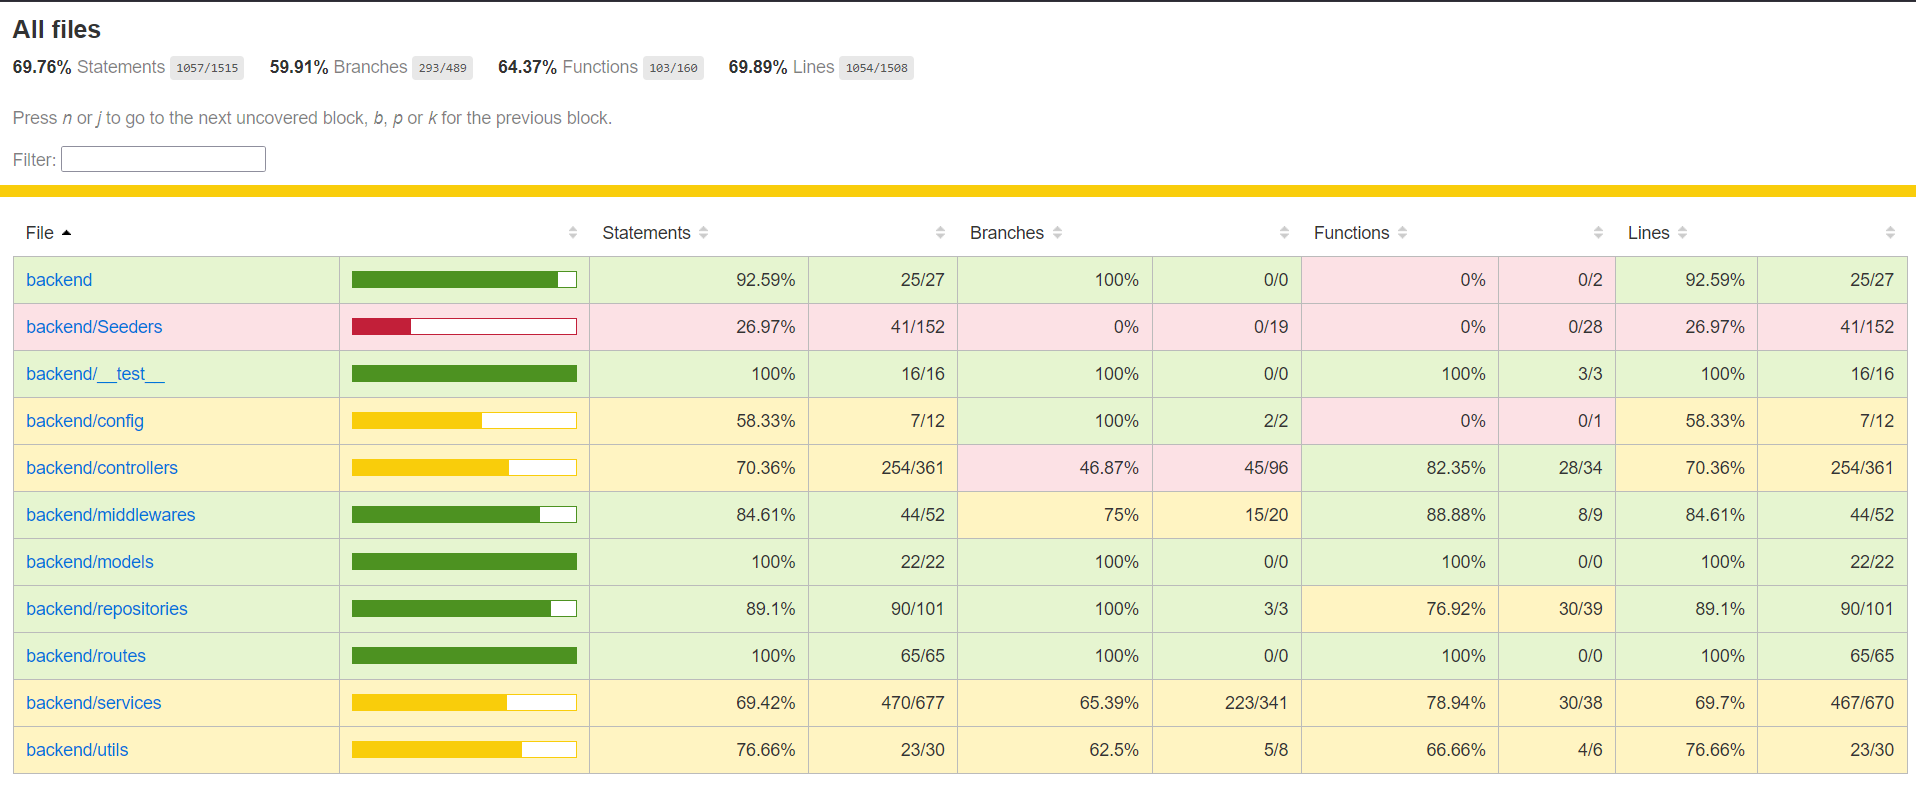
\includegraphics[clip=true,width=\textwidth]{img/cobertura_backend_logart.png}\\

    \footnotesize (f)
  \end{minipage}
  \caption{Informe de Cobertura de Pruebas del Backend (Jest).}\label{fig:coberturaBackend}
  \end{figure}

  La implementación de esta estrategia de pruebas ha sido fundamental para asegurar la calidad y estabilidad de LogArt durante su desarrollo.

\section{Distribución y Despliegue}
\label{sec:distribucionDespliegueCap4}

La capacidad de empaquetar la aplicación de forma consistente y desplegarla en diferentes entornos es crucial. LogArt utiliza Docker para la contenerización y GitHub Actions para automatizar la creación y publicación de imágenes, facilitando tanto el desarrollo local como una eventual puesta en producción.

\begin{itemize}
    \item \textbf{Empaquetado con Docker (\texttt{Dockerfile}):}
    \begin{itemize}
        \item La aplicación LogArt se empaqueta como una imagen Docker utilizando un \textbf{Dockerfile} multi-etapa, tal como se describió en la Sección \ref{sec:contenedores}.
        \item Este \texttt{Dockerfile} primero construye el frontend React en una etapa llamada (\textbf{frontend-build}, luego compila el backend Node.js en otra (\textbf{backend-build}), optimizando las dependencias y eliminando las de desarrollo.
        \item Finalmente, una etapa de producción basada en \texttt{node:20-alpine} copia los artefactos compilados del backend y el frontend (este último a una carpeta \texttt{/public} dentro del backend), resultando en una imagen final ligera y optimizada que contiene la aplicación completa lista para ejecutarse. La aplicación se configura para ejecutarse en el puerto 8443 en modo producción.
    \end{itemize}
    \vspace{0.3cm}
    \item \textbf{Orquestación Local con Docker Compose (\textbf{docker-compose.yml}):}
    \begin{itemize}
        \item Para el entorno de desarrollo local y pruebas, se utiliza el archivo detallado en la Sección \ref{ssec:arquitecturaDespliegue}: \textbf{\texttt{docker-compose.yml}} 
        \item Este archivo define y orquesta los dos servicios principales: \texttt{app} (que ejecuta la imagen Docker de LogArt) y \texttt{mongo} (que ejecuta la base de datos MongoDB).
        \item Configura las variables de entorno necesarias (cargadas desde un archivo \texttt{.env} para el servicio \texttt{app}), las redes para la comunicación entre contenedores, junto con los puertos expuestos.
        \item incluye \textit{healthchecks} para ambos servicios, asegurando un arranque ordenado y la correcta operatividad del sistema.
        \item Permite levantar todo el entorno con un simple comando (\texttt{docker-compose up}), lo que simplifica enormemente la configuración para cualquier desarrollador o para ejecutar la aplicación en un entorno de demostración. Las instrucciones detalladas para la ejecución se encuentran en el \texttt{README.md} del proyecto.
    \end{itemize}
    \vspace{0.3cm}
    \item \textbf{Distribución de Imágenes mediante CI/CD (GitHub Actions y DockerHub):}
    \begin{itemize}
        \item El proceso de construcción y distribución de la imagen Docker de LogArt está automatizado mediante el workflow de Entrega Continua en GitHub Actions, como se explicó en la Sección \ref{sec:cicd}.
        \item Cuando se publica una nueva \textit{release} en GitHub, este workflow se activa automáticamente, construye la imagen Docker de la aplicación utilizando el \texttt{Dockerfile} del proyecto.
        \item La imagen construida se etiqueta con múltiples tags (versión semántica, \texttt{latest} para releases estables, y hash del commit) y se publica en un registro público de contenedores, \textbf{DockerHub} (bajo el repositorio ``davidmorenoo/logartapp''.
        \item Esta automatización asegura que cada release estable de la aplicación esté disponible como una imagen Docker lista para ser utilizada, ya sea para despliegues manuales o mediante sistemas más avanzados.
        \item Tras la publicación de una nueva imagen, el archivo \texttt{docker-compose.yml} del proyecto (que está inicialmente configurado para usar una etiqueta específica, \texttt{latestManual}) puede ser actualizado manualmente para apuntar a la nueva versión de la imagen publicada en DockerHub si se desea utilizar la versión más reciente (última release) o apuntar a una versión anterior.
        \end{itemize}
        \vspace{0.3cm}
        \item \textbf{Consideraciones para un Futuro Despliegue en Producción (Conceptual):}
        \begin{itemize}
            \item Aunque este TFG se centra en el desarrollo y la demostración en un entorno local dockerizado, la arquitectura y el empaquetado con Docker facilitan un eventual despliegue en un entorno de producción.
            \item Se podrían utilizar plataformas de servicios en la nube que soporten contenedores Docker (ej. Amazon ECS, Google Kubernetes Engine, o plataformas PaaS como Heroku o Railway que permiten desplegar desde imágenes Docker).
            \item En un entorno de producción, se deberían utilizar certificados SSL válidos emitidos por una Autoridad de Certificación (CA) en lugar de los autofirmados, y la gestión de secretos (como claves de API, contraseñas de base de datos, etc) se realizaría mediante sistemas de gestión de secretos específicos de la plataforma de nube utilizada, o herramientas como HashiCorp Vault.
            \item La base de datos MongoDB podría desplegarse como un servicio gestionado (ej. MongoDB Atlas) para mayor escalabilidad y resiliencia.
        \end{itemize}
\end{itemize}

Este enfoque de distribución y despliegue basado en contenedores y CI/CD asegura la reproducibilidad, facilita la gestión de la aplicación y sienta las bases para una operativa futura eficiente.

\blankpage

% Capítulo 5

\chapter{Conclusiones y Trabajos Futuros}
\label{chap:conclusiones}
Tras el detallado recorrido por la especificación, diseño, implementación y validación de la aplicación ``LogArt: Galería de Recuerdos'' expuesto en los capítulos anteriores, este capítulo final tiene como propósito consolidar las principales conclusiones extraídas del desarrollo de este Trabajo de Fin de Grado. Se realizará una evaluación del cumplimiento de los objetivos inicialmente planteados, se reflexionará sobre los desafíos encontrados y los aprendizajes adquiridos durante el proceso, y se presentará una visión sobre las posibles líneas de evolución y trabajos futuros que podrían enriquecer y expandir la funcionalidad de LogArt.

Este capítulo busca, por tanto, no solo resumir los resultados del proyecto, sino también ofrecer una perspectiva personal sobre la experiencia de desarrollo y el potencial de la aplicación creada.

\section{Conclusiones del Proyecto}
\label{sec:conclusionesProyecto}

El desarrollo de ``LogArt: Galería de Recuerdos'' ha culminado en una aplicación web funcional que satisface la necesidad principal de proporcionar a los usuarios una plataforma personal para documentar y organizar sus experiencias y recuerdos relacionados con diversas disciplinas culturales. A continuación, se evalúa el proyecto en función de sus objetivos, los resultados obtenidos y los desafíos enfrentados.

\subsection{Cumplimiento de Objetivos}
\label{ssec:cumplimientoObjetivos}

El proyecto se planteó como una serie de objetivos tanto generales como específicos, detallados en el Capítulo \ref{chap:objetivos}. Se puede concluir que estos objetivos han sido alcanzados satisfactoriamente:
\begin{itemize}
    \item \textbf{Objetivo Principal:} Se ha diseñado, desarrollado e implementado con éxito LogArt, una aplicación web SPA funcional que permite a los usuarios registrar, organizar y consultar sus recuerdos culturales. La aplicación ofrece las herramientas necesarias para gestionar galerías personales de libros, canciones y videojuegos, y detallar experiencias mediante comentarios.
    \item \textbf{Objetivos Específicos:}
    \begin{itemize}
        \item \textbf{Análisis y Definición de Requisitos (OE1):} Se llevó a cabo un análisis de las funcionalidades necesarias, resultando en la especificación detallada de requisitos presentada en el Capítulo \ref{chap:descripcionInformatica}.
        \item \textbf{Diseño de la Arquitectura (OE2):} Se diseño e implementó una arquitectura basada en el stack MERN (MongoDB, Express.js, React y Node.js), que demostró ser adecuada para los requisitos del proyecto, permitiendo un desarrollo fullstack JavaScript coherente.
        \item \textbf{Desarrollo del Backend (OE3):} Se construyó una API RESTful robusta con Express.js y Node.js, gestionando la lógica de negocio y la persistencia de datos en MongoDB mediante Mongoose.
        \item \textbf{Desarrollo del Frontend (OE4):} Se desarrolló una interfaz de usuario interactiva y responsiva como una Single Page Application (SPA) utilizando React, facilitando una experiencia de usuario fluida.
        \item \textbf{Implementación de Funcionalidades Clave (OE5):} Se implementaron todas las funcionalidades esenciales definidas, incluyendo la gestión completa de usuarios (registro, login, perfiles), el ciclo CRUD para objetos y comentarios, la categorización por disciplinas, y funcionalidades avanzadas como la compartición de objetos, sistema de favoritos, notificaciones en tiempo real, y un panel de administración con estadísticas y herramientas de moderación.
        \item \textbf{Pruebas y Validación (OE6):} Se estableció una estrategia de pruebas automáticas que incluye pruebas de integración para el backend (Jest y Supertest) y pruebas End-To-End para el frontend (Playwright), contribuyendo significativamente a la calidad y estabilidad de la aplicación.
        \item \textbf{Contenerización y Despliegue (OE7):} La aplicación fue completamente contenerizada utilizando Docker y Docker Compose, simplificando su configuración y ejecución. Además, se implementó un pipeline de Integración Continua y Entrega Continua (CI/CD) con Github Actions para automatizar las pruebas y la publicación de imágenes Docker en DockerHub.
        \item \textbf{Elaboración de la Documentación (OE8):} Se ha completado la presente memoria de Trabajo de Fin de Grado, documentando exhaustivamente el proceso de desarrollo, las decisiones tomadas y los resultados obtenidos.
    \end{itemize}
\end{itemize}

En resumen, la aplicación LogArt desarrollada cumple con el conjunto de objetivos, funcionalidades y características técnicas que se propusieron como metas del proyecto.

\subsection{Resultados Obtenidos}
\label{ssec:resultadosObtenidos}

El principal resultado de este TFG es la aplicación web LogArt, una plataforma operativa que ofrece una solución viable y útil para aquellos usuarios que deseen llevar un registro personal y detallado de su consumo cultural.

\subsection{Desafíos Enfrentados y Soluciones}
\label{ssec:desafiosSoluciones}

Durante el desarrollo de LogArt, se presentaron diversos desafíos técnicos y de aprendizaje, cuya superación fue clave para el éxito del proyecto:
\begin{itemize}
    \item \textbf{Adopción y Dominio del Stack MERN Completo:} Si bien se tenían conocimientos previos de algunas tecnologías, la integración y el dominio profundo de todo el stack MERN (especialmente la interacción eficiente entre React, Node.js/Express.js y MongoDB con Mongoose) supuso una curva de aprendizaje continua. Se abordó mediante estudio autodidacta, consulta de documentación oficial y experimentación práctica. Por este mismo motivo, y por ser el primer proyecto en el stack MERN realizado por el tutor, el código puede no ser lo más óptimo posible.
    \item \textbf{Diseño de una API RESTful Coherente y Segura:} Definir una API que fuera a la vez intuitiva, segura (con autenticación JWT y autorización por roles) y que cubriera todas las necesidades funcionales requirió un diseño iterativo y cuidadoso.
    \item \textbf{Implementación del Panel de Administración:} El desarrollo del dashboard de administrador, con sus diversas estadísticas y agregaciones de datos, representó un desafío significativo en términos de lógica de backend y presentación de datos en el frontend. Se superó mediante la descomposición del problema en consultas más pequeñas y la construcción incremental de la interfaz.
    \item \textbf{Configuración de CI/CD y Dockerización Completa:} Asegurar que la aplicación se construyera correctamente en contenedores Docker y que los pipelines de CI/CD funcionaran de manera fiable para las pruebas y la publicación de imágenes implicó un aprendizaje considerable sobre Docker, Docker Compose y GitHub Actions, especialmente en la gestión de dependencias y entornos.
\end{itemize}
La resolución de estos desafíos fue fundamental no solo para el proyecto en sí, sino también para el desarrollo de habilidades de resolución de problemas y la consolidación de conocimientos técnicos.

\subsection{Limitaciones del Proyecto y Trabajos Futuros}
\label{ssec:limitacionesproyecto}

A pesar de los logros alcanzados, es importante reconocer algunas limitaciones del proyecto LogArt en su estado actual, que podrían abordarse en futuras iteraciones:
\begin{itemize}
    \item \textbf{Cobertura de Pruebas:}
    Aunque se implementó una base sólida de pruebas, la cobertura de código (aproximadamente 70\%, Sección \ref{sec:pruebasCap4}) podría incrementarse, para aumentar más la robustez del sistema.
    \item \textbf{Almacenamiento de Imágenes:} Actualmente, las imágenes subidas por los usuarios se almacenan en el sistema de ficheros del servidor donde se ejecuta la aplicación. Para una mayor escalabilidad, resiliencia y eficiencia en un entorno de producción, sería preferible integrar un servicio de almacenamiento en la nube (Amazon S3 o Google Cloud Storage).
    \item \textbf{Despliegue en Producción:} Si bien la aplicación está completamente dockerizada y lista para ser desplegada, este TFG no ha incluido la puesta en producción en un servidor público o plataforma en la nube.
\end{itemize}
Estas limitaciones no demeritan el trabajo realizado, sino que motivan y ofrecen un punto de partida claro para futuras mejoras y desarrollos.

\section{Reflexión Personal y Aprendizaje}
\label{sec:reflexionPersonal}

La realización del Trabajo Fin de Grado ``LogArt: Galería de Recuerdos" ha constituido una experiencia de aprendizaje sumamente valiosa y enriquecedora, tanto a nivel técnico como personal. Este proyecto ha representado la culminación de los conocimientos adquiridos durante el Grado en Ingeniería del Software y una oportunidad para aplicarlos en un desarrollo completo y autónomo.

Desde el punto de vista \textbf{técnico}, el TFG ha permitido profundizar y consolidar habilidades en un espectro amplio de tecnologías modernas para el desarrollo web FullStack. Destaca el aprendizaje práctico y la aplicación del stack MERN (MongoDB, Express.js, React, Node.js), la implementación de arquitecturas RESTful, y la interacción con bases de datos NoSQL. Igualmente significativo ha sido el dominio de herramientas y prácticas DevOps, como la contenerización con Docker y Docker Compose, la configuración de pipelines de Integración Continua y Entrega Continua (CI/CD) con GitHub Actions, y la implementación de una estrategia de pruebas automáticas multinivel (unitaria, integración y E2E).

A nivel \textbf{personal y profesional}, el proyecto ha fomentado el desarrollo de habilidades cruciales como la planificación y gestión autónoma de un proyecto de software de principio a fin, la toma de decisiones fundamentadas, la resolución de problemas complejos bajo plazos definidos, y la capacidad de crear documentación técnica. Además, la necesidad de investigar, aprender y superar obstáculos de forma independiente, ha reforzado la proactividad y la resiliencia del autor.

En definitiva, el desarrollo de LogArt ha sido un desafío, que no solo ha resultado en una aplicación funcional, sino que también ha servido como un excelente campo de pruebas para solidificar mi formación como futuro Ingeniero del Software.

\blankpage


%%%%%%%%%%%%%%%%%%%%%%%%%%%%%%% Bibliografía %%%%%%%%%%%%%%%%%%%%%%%%%%%%%%%

\phantomsection
\addcontentsline{toc}{chapter}{Bibliografía}

\footnotesize{
%\bibliographystyle{hispa}
\bibliographystyle{IEEEtran}
\bibliography{bibliografia}
}



% No expandir elementos para llenar toda la página
\raggedbottom
\afterpage{\blankpage}

\newpage




%%%%%%%%%%%%%%%%%%%%%%%%%%%%%%% Apéndices %%%%%%%%%%%%%%%%%%%%%%%%%%%%%%%

\appendix

\phantomsection
\addcontentsline{toc}{chapter}{Apéndices}

\mbox{}
\vfill
\begin{center}
\begin{Huge}
\textbf{Apéndices}
\end{Huge}
\end{center}
\vfill
\mbox{}
\thispagestyle{empty}

\newpage
\mbox{}
\thispagestyle{empty}
\newpage



\chapter{Primer Apéndice: Construcción e instalación del software}
\label{chap:apendiceConstruccion}
El presente anexo detalla los pasos necesarios para obtener el código fuente de la aplicación LogArt, configurar el entorno y ejecutar la aplicación en un entorno local utilizando Docker y Docker Compose.

\section{Requisitos Previos}
\label{appA:requisitosPrevios}

Antes de continuar, asegúrese de tener instaladas las siguientes herramientas en el sistema:
\begin{itemize}
    \item \textbf{Git:} Para clonar el repositorio del proyecto. (Guía de instalación disponible en \url{https://git-scm.com/book/en/v2/Getting-Started-Installing-Git})
    \item \textbf{Docker Engine:} Para construir y ejecutar los contenedores de la aplicación. (Guía de instalación: \url{https://docs.docker.com/get-docker/})
    \item \textbf{Docker Compose:} Para orquestar la aplicación multi-contenedor. (Guía de instalación: \url{https://docs.docker.com/compose/install/})
\end{itemize}
Se recomienda utilizar versiones recientes de Docker y Docker Compose (ej. Docker +v24.x, Docker Compose con sintaxis +v3.8).

\section{Obtención del Código Fuente}
\label{appA:obtencionCodigo}

El código fuente de LogArt está alojado en un repositorio de GitHub. Para obtenerlo, clone el repositorio utilizando el siguiente comando en su terminal Git:
\begin{verbatim}
    git clone https://github.com/codeurjc-students/2024-logart.git
\end{verbatim}

Una vez clonado, navegue al directorio específico donde se encuentra el archivo \texttt{Dockerfile}, que para este proyecto es \texttt{LogArtApp/docker/} dentro del repositorio clonado:
\begin{verbatim}
    cd 2024-logart/LogArtApp/docker/
\end{verbatim}

\section{Configuración del Entorno (\texttt{.env})}
\label{appA:configuracionEntorno}
LogArt requiere un archivo de configuración de entorno llamado \texttt{.env} para definir variables críticas como las credenciales de la base de datos, configuración de correo electrónico y secretos de la aplicación. Este archivo debe ser creado por el usuario que va a construir e instalar la aplicación, en el directorio \texttt{LogArtApp/docker/} (el mismo directorio donde se encuentra el archivo \texttt{docker-compose.yml}.

Cree entonces un archivo llamado \texttt{.env} en ese directorio y añada el siguiente contenido, \textbf{reemplazando los valores placeholder (your\_...)} con sus propias credenciales o valores deseados:

\begin{verbatim}
# MongoDB Configuration (credenciales para el usuario root de MongoDB)
MONGO_INITDB_ROOT_USERNAME=your_mongo_root_user
MONGO_INITDB_ROOT_PASSWORD=your_mongo_root_password

# Backend Database Connection String (usa las credenciales anteriores)
DB_CONNECTION_STRING=mongodb://your_mongo_root_user
:your_mongo_root_password@mongo:27017/logartdb?authSource=admin

# JWT Configuration (usar cadenas largas y aleatorias)
ACCESS_TOKEN_SECRET=your_very_strong_and_random_access_token_secret

# Email Configuration (para verificación de cuenta y recuperación de contraseña)
EMAIL_USER=your_gmail_address_for_sending_emails@gmail.com
EMAIL_PASS=your_gmail_app_password_or_regular_password 
# Nota: Para Gmail, se debe usar una "Contraseña de aplicación".

# Application Configuration
BASE_URL=https://localhost:8443 # URL base donde la aplicación será accesible
PORT=8443 # Puerto en el que escuchará el servidor Node.js dentro del contenedor
NODE_ENV=production # Entorno de ejecución de Node.js

# SSL Configuration (rutas relativas al directorio del backend dentro del contenedor)
SSL_KEY_PATH=ssl/server.key
SSL_CERT_PATH=ssl/server.cert
\end{verbatim}

\textbf{Nota Importante sobre SSL para Ejecución Local:}
La aplicación está configurada para utilizar HTTPS. El \texttt{Dockerfile} (etapa \texttt{backend-build}) no incluye la generación de certificados SSL autofirmados, estos deben ser creados y proporcionados. Para desarrollo local, deberá:
\begin{enumerate}
    \item Crear un directorio \textbf{ssl} dentro de \texttt{LogArtApp/backend/}.
    \item Generar sus propios archivos \texttt{server.key} y \texttt{server.cert} autofirmados (por ejemplo, usando OpenSSL) y colocarlos en la carpeta mencionada (\texttt{LogArtApp/backend/ssl/}.
\end{enumerate}
Alternativamente, si no se desea usar HTTPS, ni configurar SSL, y únicamente para un entorno de desarrollo local estricto, sería necesario modificar el código del servidor Express.js (\texttt{backend/server.js}) para que escuche sobre HTTP en lugar de HTTPS, lo cual no es recomendado. \textbf{No se asegura el correcto funcionamiento de la web y sus contenidos asociados usando HTTP}.

\section{Ejecución de la Aplicación}
\label{appA:ejecucionApp}

Una vez clonado el repositorio, configurado el archivo \texttt{.env} en el directorio \texttt{LogArtApp/docker/}, y preparados los certificados SSL, existen dos métodos principales para ejecutar la aplicación LogArt utilizando Docker.

\subsection{Método 1: Construcción Manual de la Imagen y Ejecución con Docker Compose}
\label{appA:ejecucionMetodo1}
Este método es útil si se desea construir la imagen Docker localmente a partir del código fuente más reciente o con modificaciones propias antes de levantar los servicios.
\begin{enumerate}
    \item \textbf{Construir la Imagen Docker Localmente:}
    Navegue al directorio raíz del proyecto clonado (\texttt{2024-logart/LogArtApp/}). Desde allí, ejecute el siguiente comando para construir la imagen Docker utilizando el \texttt{Dockerfile} ubicado en la carpeta \texttt{LogArtApp/docker/Dockerfile}. Puede asignar el tag que desee:
    \begin{verbatim}
        docker build -t davidmorenoo/logartapp:latestManual -f docker/Dockerfile .
    \end{verbatim}
    \textbf{Nota:} Si utiliza un tag diferente al que está especificado en el archivo \texttt{docker-compose.yml}, deberá actualizar la directiva \texttt{image} del servicio \texttt{app} en el archivo \texttt{docker-compose.yml} para que coincida con el tag de la imagen que acaba de construir.
    \item \textbf{Levantar los Servicios con Docker Compose:}
    Navegue al directorio \texttt{LogArtApp/docker/} (donde se encuentra el archivo \texttt{docker-compose.yml} y su \texttt{.env} configurado). Ejecute el siguiente comando para iniciar todos los servicios (la aplicación LogArt y la base de datos MongoDB):
    \begin{verbatim}
        docker compose up
    \end{verbatim}
\end{enumerate}

\subsection{Método 2: Ejecución Directa con Docker Compose (Utilizando Imagen Pre-construida}
\label{appA:ejecucionMetodo2}
Este método es el recomendado, ya que es más directo, al estar el \texttt{docker-compose.yml} configurado para utilizar una imagen pre-construida de DockerHub.
\begin{enumerate}
    \item \textbf{Asegurar Configuración del \texttt{docker-compose.yml}:}
    Verifique que el archivo \texttt{docker-compose} esté correctamente configurado. Por defecto, el servicio \texttt{app} utiliza la imagen \texttt{latestManual} disponible en el repositorio público \texttt{davidmorenoo/logartapp} de DockerHub.
    \item \textbf{Levantar los Servicios con Docker Compose:}
    Navegue al directorio \texttt{LogArtApp/docker/} y ejecute el siguiente comando:
    \begin{verbatim}
        docker compose up
    \end{verbatim}
\end{enumerate}

\subsection{Acceso a la Aplicación}
\label{appA:accesoApp}
Independientemente del método de ejecución elegido, una vez que los contenedores estén en funcionamiento, la aplicación LogArt estará disponible en el navegador web a través de la URL:
\begin{center}
    \url{https://localhost:8443}
\end{center}
\textbf{Nota sobre Certificados SSL Autofirmados:} Al utilizar certificados SSL autofirmados para el desarrollo local sobre HTTPS, es probable que su navegador muestre una advertencia de seguridad. Deberá aceptar a través de las opciones de ``configuración avanzada'' para acceder al sitio (generalmente buscando una opción como ``Acceder a localhost (sitio no seguro)'' o similar).

\section{Detener la Aplicación}
\label{appA:detenerApp}
Para detener todos los servicios de la aplicación (LogArt y MongoDB) y eliminar los contenedores, navegue al directorio \texttt{LogArtApp/docker/} y ejecute:
\begin{verbatim}
    docker compose down
\end{verbatim}
Si desea volver a iniciar la aplicación, puede ejecutar nuevamente \texttt{docker compose up}.

\textbf{Credenciales de Acceso de Ejemplo y Datos Precargados}
\label{appA:credencialesDatos}
LogArt se inicia con un conjunto de datos de ejemplo y credenciales predefinidas para facilitar la exploración y testeo inicial:

\begin{itemize}
    \item \textbf{Usuario Administrador:}
    \begin{itemize}
        \item \textbf{Username/Email:}
        \texttt{admin@gmail.com}
        \item \textbf{Password:} \texttt{admin123}
        \item \textbf{Permisos:} Acceso completo a todas las funcionalidades, incluyendo el panel de administración, la moderación de contenido y el resto de funcionalidades definidas para usuario administrador en \ref{ssec:actoresSistema}
    \end{itemize}
    \item \textbf{Usuario Registrado:}
    \begin{itemize}
        \item \textbf{Username/Email:}
        \texttt{pepe@gmail.com}
        \item \textbf{Password:} \texttt{hola123}
        \item \textbf{Permisos:} Creación y gestión de sus propios objetos y comentarios, junto con el resto de funcionalidades definidas para usuario registrado en \ref{ssec:actoresSistema}
    \end{itemize}
    \item \textbf{Usuario No Registrado:}
        \begin{itemize}
            \item Puede visualizar la página principal y los objetos que hayan sido compartidos públicamente por otros usuarios, junto con el resto de funcionalidades definidas para usuario no registrado en \ref{ssec:actoresSistema}
        \end{itemize}
\end{itemize}

La aplicación también incluye datos de ejemplo preconfigurados para las disciplinas (Videojuegos, Libros, Canciones), algunos objetos y comentarios, que pueden ser modificados o eliminados por los usuarios o por el administrador.

\section{Interacción con la Base de Datos (Opcional para Desarrollo Avanzado)}
\label{appA:interaccionBD}
Si desea realizar depuración avanzada, y necesita interactuar con la base de datos MongoDB que se ejecuta en el contenedor, puede hacerlo. Con los contenedores en ejecución (tras un \texttt{docker compose up}, abra una terminal y ejecute el siguiente comando para acceder al shell de MongoDB dentro del contenedor \texttt{mongo}. Deberá reemplazar \texttt{your\_mongo\_root\_user} y \texttt{your\_mongo\_root\_password} con los valores que configuró en su archivo \texttt{.env}:
\begin{verbatim}
    docker exec -it docker-mongo-1 mongosh \
   --username your_mongo_root_user \
   --password your_mongo_root_password \
   --authenticationDatabase admin
\end{verbatim}
Una vez dentro del shell de \texttt{mongosh}, puede ejecutar comandos de MongoDB. Por ejemplo, para ver los objetos en la base de datos de LogArt:
\begin{verbatim}
    use logartdb;
    show collections;
    db.objects.find().pretty();
\end{verbatim}
Este acceso directo a la base de datos debe realizarse con cuidado, y solo en casos de depuración avanzada.

\chapter{Segundo Apéndice: Manual de Usuario Básico}
\label{chap:manualUsuario}
El presente manual proporciona una guía básica para que los nuevos usuarios puedan comenzar a utilizar la aplicación ``LogArt: Galería de Recuerdos'' y aprovechar sus funcionalidades principales.

\section{Acceso a la Aplicación}
\label{appB:acceso}
Para acceder a LogArt, abra su navegador web y diríjase a la URL donde la aplicación ha sido desplegada (\ref{appA:ejecucionApp}).
\begin{itemize}
    \item \textbf{Página de Inicio (Hero):} Si no ha iniciado sesión, verá la página de inicio, que presenta información general sobre LogArt y una sección de Preguntas Frecuentes (FAQs). Desde aquí, podrá optar por registrarse o iniciar sesión. Figura \ref{fig:pantallaHero}

    \begin{figure}
   \centering

  \begin{minipage}{0.45\textwidth}
   \centering

     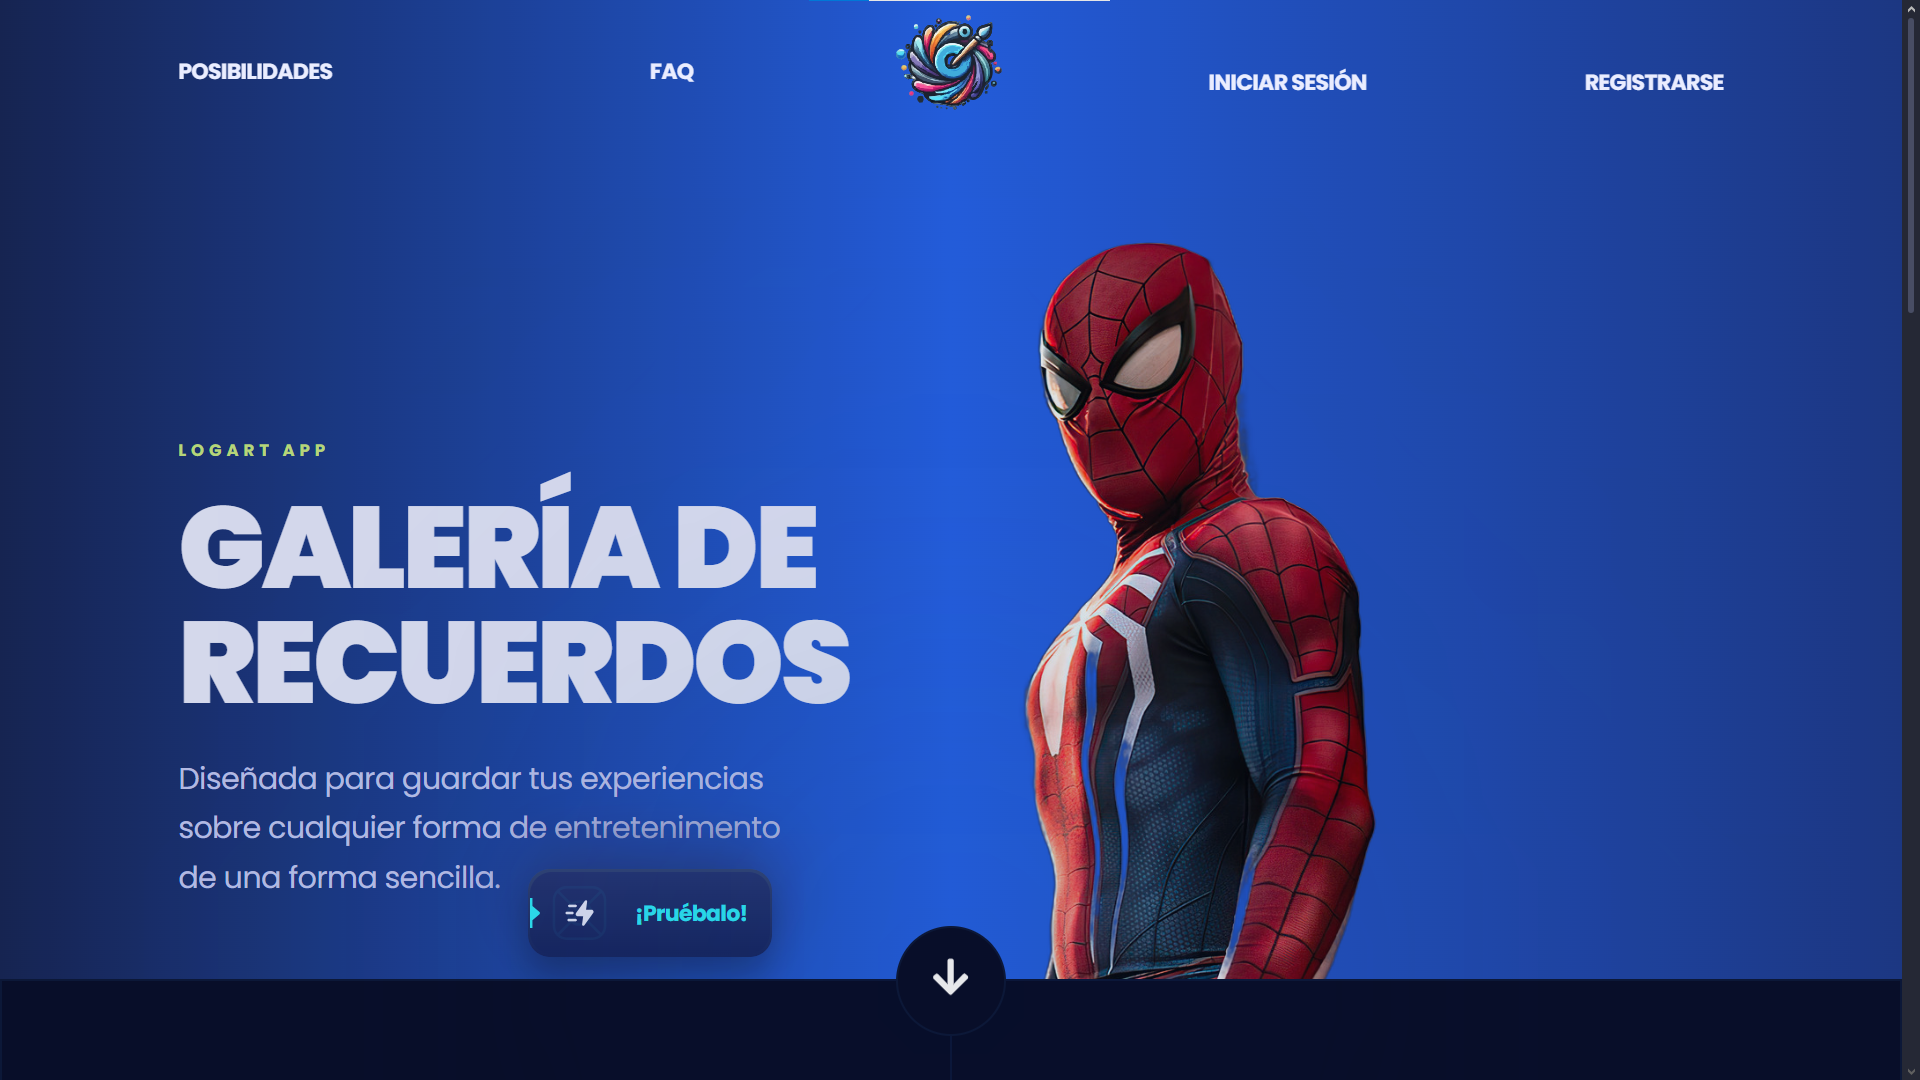
\includegraphics[clip=true,width=\textwidth]{img/hero1home.png}\\

    \footnotesize (g)
  \end{minipage}
  \caption{Pantalla Hero (home).}\label{fig:pantallaHero}
  \end{figure}
  
    \item \textbf{Usuarios Anónimos:} Como usuario no registrado, puede explorar los objetos que otros usuarios hayan decidido compartir públicamente, siempre y cuando tenga el link disponible. Figura \ref{fig:pantallaObjetoDetalle}
\end{itemize}

\section{Registro de una Nueva Cuenta}
\label{appB:registro}
Para utilizar todas las funcionalidades de LogArt, como crear sus propias galerías y objetos, necesitará registrarse. Figura \ref{fig:pantallaRegistro}
\begin{enumerate}
    \item En la página de inicio o desde el menú de navegación, haga clic en la opción "Registrarse".
    \item Complete el formulario de registro proporcionando:
    \begin{itemize}
        \item Nombre de Usuario.
        \item Nombre.
        \item Apellidos.
        \item Dirección de Correo Electrónico (válida).
        \item Contraseña.
    \end{itemize}
    \item Tras enviar el formulario, recibirá un correo electrónico en la dirección proporcionada con un enlace para verificar su cuenta.
    \item Haga clic en el enlace de verificación en el correo para activar su cuenta. Este paso es obligatorio para poder iniciar sesión.
\end{enumerate}
\begin{figure}
   \centering

  \begin{minipage}{0.45\textwidth}
   \centering

     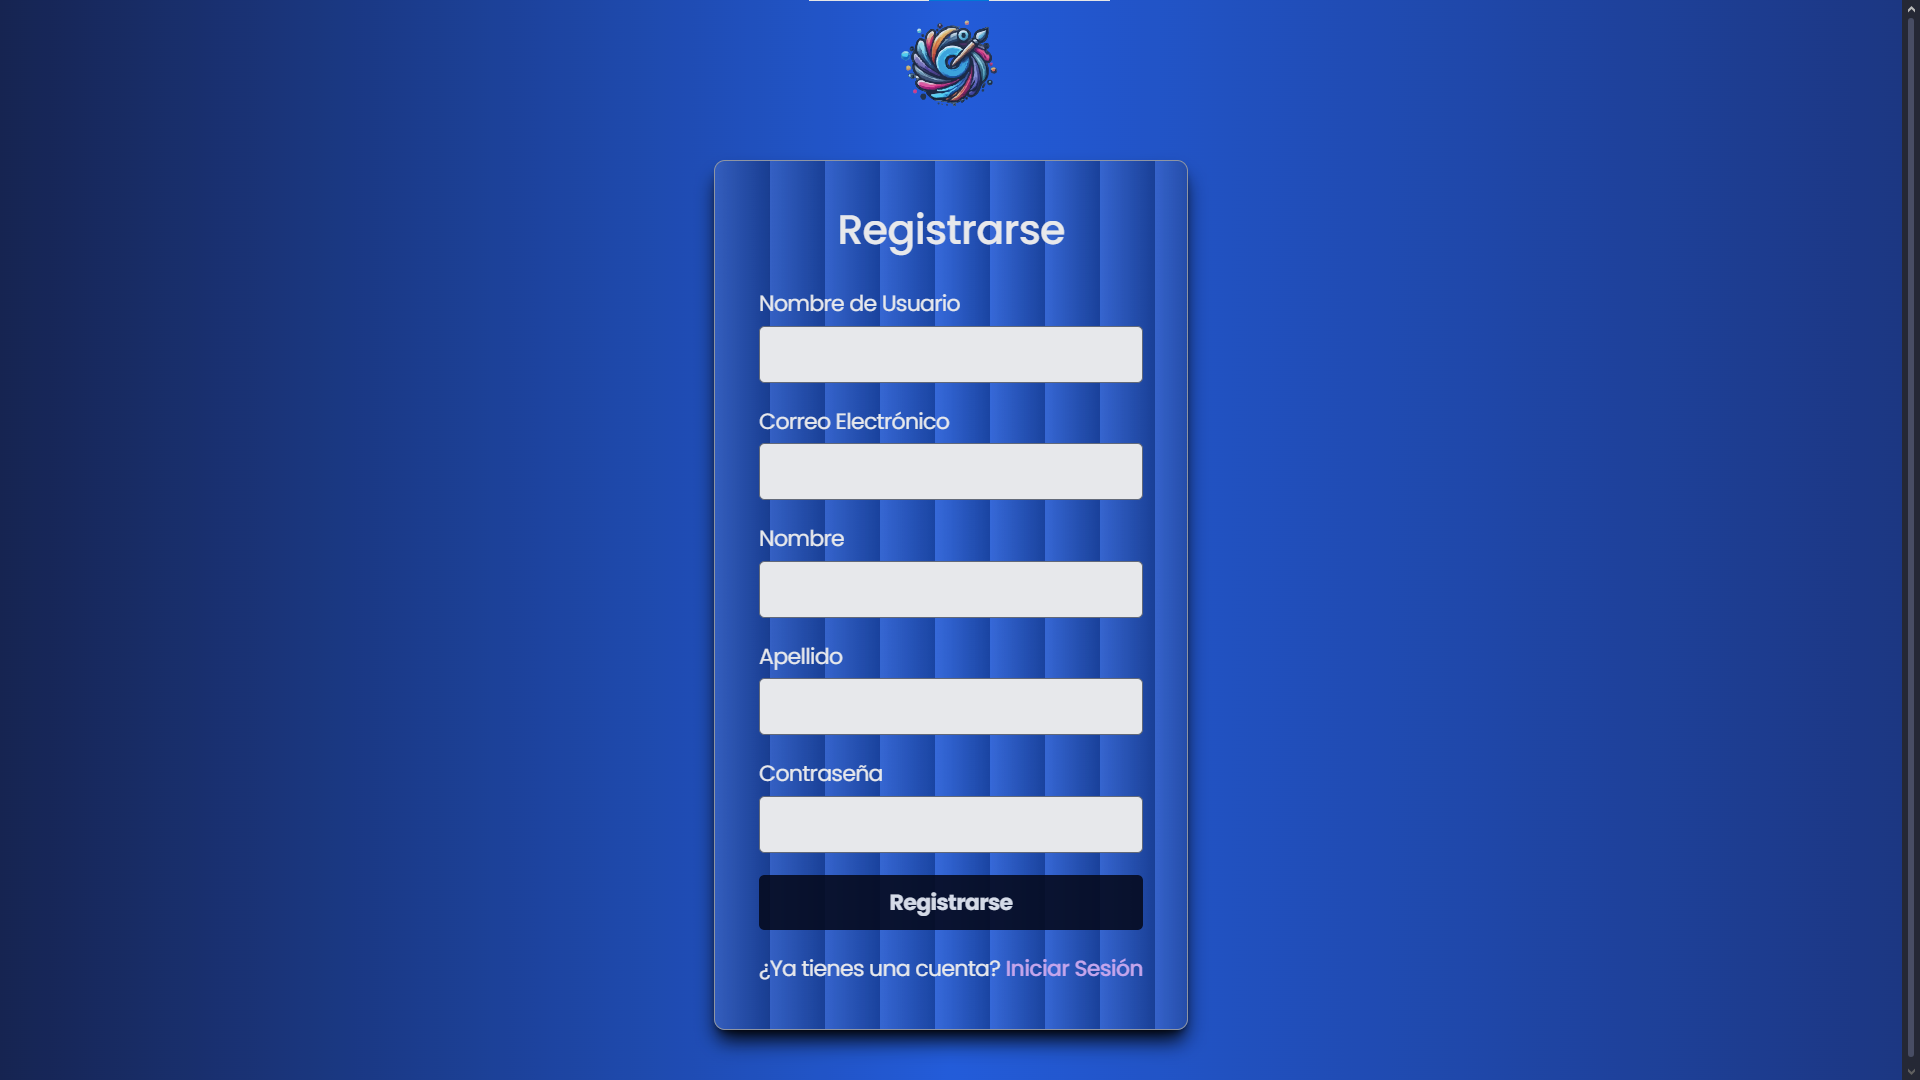
\includegraphics[clip=true,width=\textwidth]{img/register.png}\\

    \footnotesize (h)
  \end{minipage}
  \caption{Pantalla Registro.}\label{fig:pantallaRegistro}
  \end{figure}

\section{Inicio de Sesión}
\label{appB:inicioSesion}
Una vez que su cuenta esté verificada: Figura \ref{fig:pantallaLogin}
\begin{enumerate}
    \item Haga clic en la opción ``Iniciar Sesión'' (Login) desde la página de inicio, o en el menú de navegación.
    \item Ingrese su correo electrónico y la contraseña con la que se registró.
    \item Si las credenciales son correctas, accederá a su panel personal de LogArt.
\end{enumerate}
\textbf{Recuperación de Contraseña:} Si olvida su contraseña, puede utilizar la opción ``¿Olvidaste tu contraseña?'' en la página de inicio de sesión para iniciar el procedimiento de restablecimiento a través de su correo electrónico. Figura \ref{fig:pantallaLogin}

\begin{figure}
   \centering

  \begin{minipage}{0.45\textwidth}
   \centering

     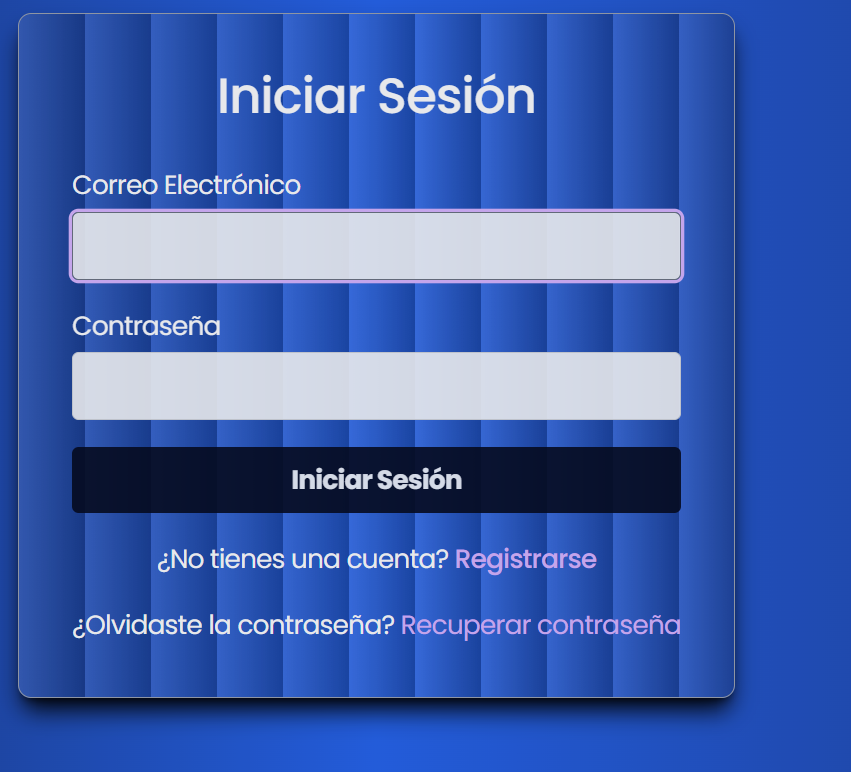
\includegraphics[clip=true,width=\textwidth]{img/pass1.png}\\

    \footnotesize (i)
  \end{minipage}
  \caption{Pantalla de Inicio de Sesión.}\label{fig:pantallaLogin}
  \end{figure}

\section{Navegación Principal y Galerías}
\label{appB:navegacionGalerias}
Una vez iniciada la sesión: Figura \ref{fig:pantallaGaleria}
\begin{itemize}
    \item \textbf{Selección de Disciplina:} Se le presentará la pantalla de galerías, con un selector para seleccionar una disciplina (Libros, Canciones, Videojuegos) para acceder a su galería personal correspondiente. Puede cambiar entre estas galerías de diferentes disciplinas utilizando el mismo selector.
    \item \textbf{Vista de Galería:} Muestra todos los objetos que ha creado para la disciplina seleccionada. Puede buscar objetos por nombre o filtrar para ver solo sus favoritos. Si tiene muchos objetos, la galería se mostrará paginada.
\end{itemize}


\section{Gestión de Objetos}
\label{appB:gestionObjetos}
\begin{itemize}
    \item \textbf{Crear un Nuevo Objeto:}
    \begin{enumerate}
        \item En la vista de galería, haga clic en el botón verde ``Crear Objeto''. Figura \ref{fig:pantallaGaleria}
        \item Se abrirá un formulario modal donde deberá ingresar:
        \begin{itemize}
            \item Nombre del objeto.
            \item Descripción.
            \item Disciplina.
            \item Una imagen representativa para el objeto.
        \end{itemize}
        \item Haga clic en ``Crear'' para guardar el objeto en su galería.
    \end{enumerate}
    \item \textbf{Ver Detalles de un Objeto:} Haga clic en el nombre o la imagen de un objeto en la galería para acceder a su vista detallada. Aquí verá toda su información y los comentarios asociados. Figura \ref{fig:pantallaObjetoDetalle}
    \item \textbf{Editar un Objeto:} Si es el propietario del objeto, en la tarjeta del objeto encontrará una opción para ``Editar''. Esto abrirá un formulario similar al de creación para modificar sus datos. \ref{fig:pantallaGaleria}
    \item \textbf{Eliminar un Objeto:} Si es el propietario del objeto, podrá eliminar un objeto desde su tarjeta en la galería, con un botón similar al de ``Editar'', pero con el texto ``Eliminar'' y en rojo. Se le pedirá confirmación antes de la eliminación. Figura \ref{fig:pantallaGaleria}
\end{itemize}

\begin{figure}
   \centering

  \begin{minipage}{0.45\textwidth}
   \centering

     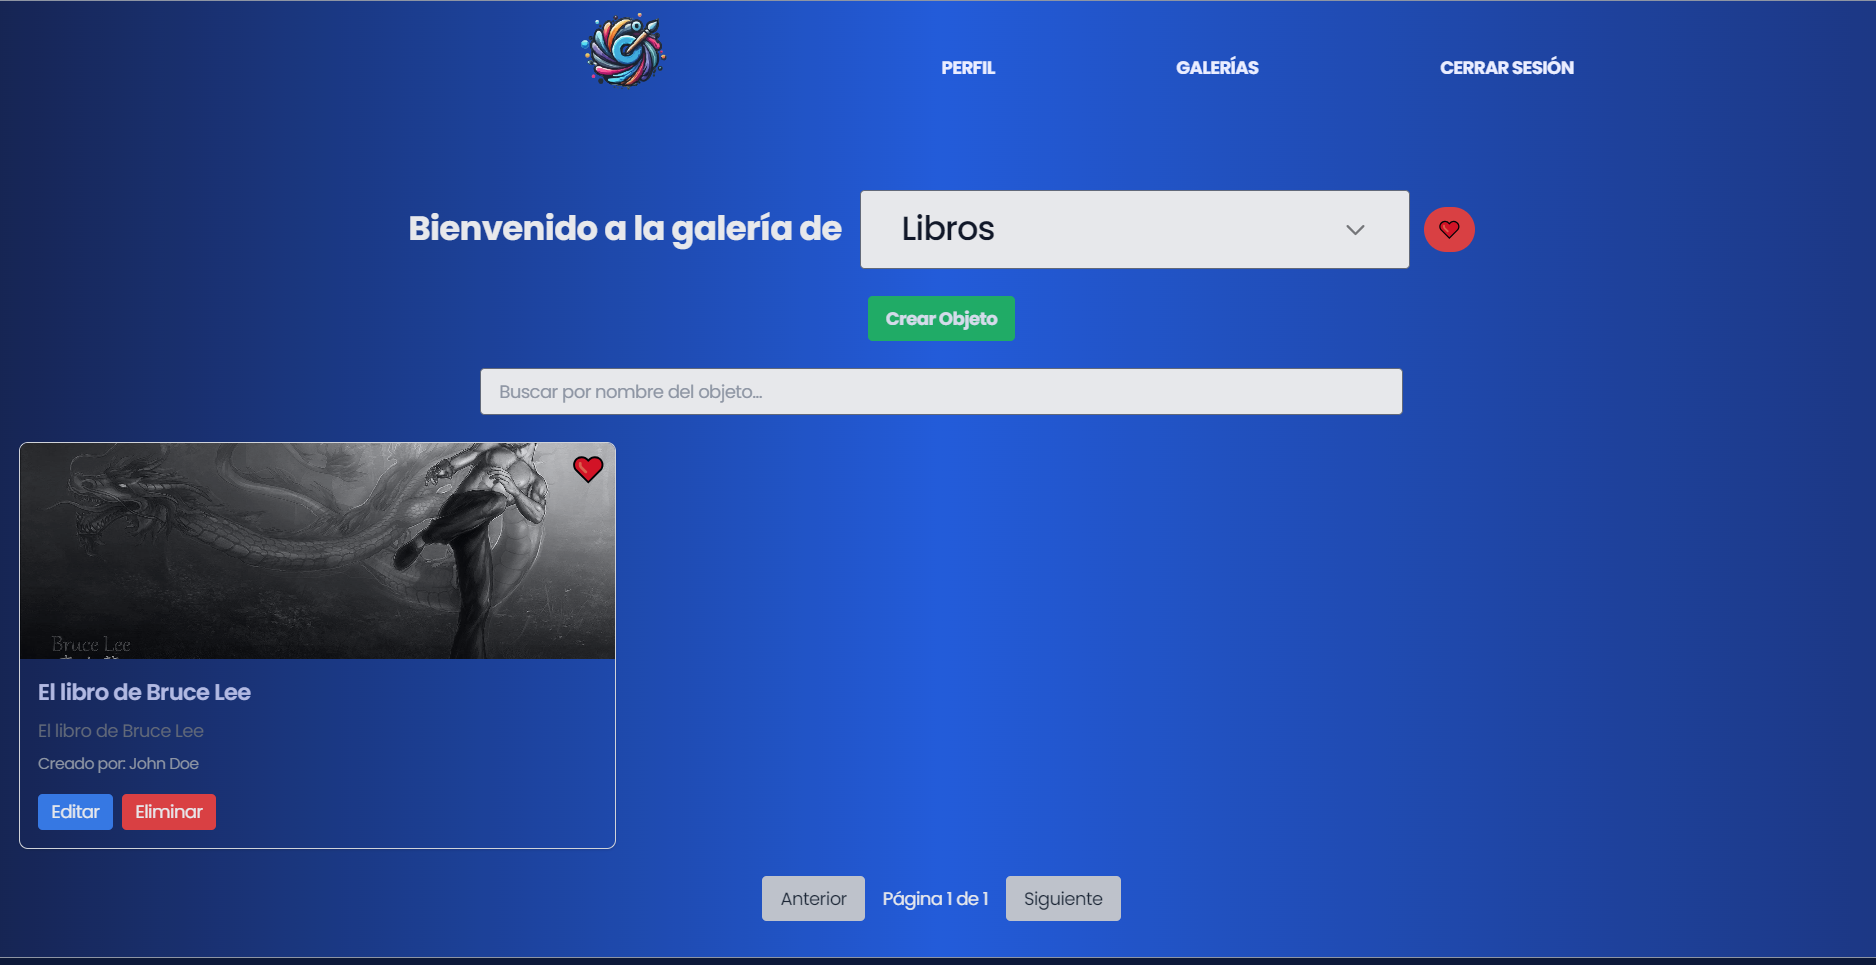
\includegraphics[clip=true,width=\textwidth]{img/fav2.png}\\

    \footnotesize (j)
  \end{minipage}
  \caption{Pantalla de Galería de Objetos.}\label{fig:pantallaGaleria}
  \end{figure}

\section{Gestión de Comentarios}
\label{appB:gestionComentarios}
Los comentarios le permiten añadir sus recuerdos y experiencias detalladas a cada objeto.
\begin{itemize}
    \item \textbf{Añadir un Comentario:} En la vista detallada de un objeto de su propiedad, encontrará una sección para escribir y guardar nuevos comentarios.
    \item \textbf{Editar / Eliminar Comentarios:} Si es el autor del comentario, o un administrador, podrá editar su contenido o eliminarlo.
\end{itemize}

\begin{figure}
   \centering

  \begin{minipage}{0.45\textwidth}
   \centering

     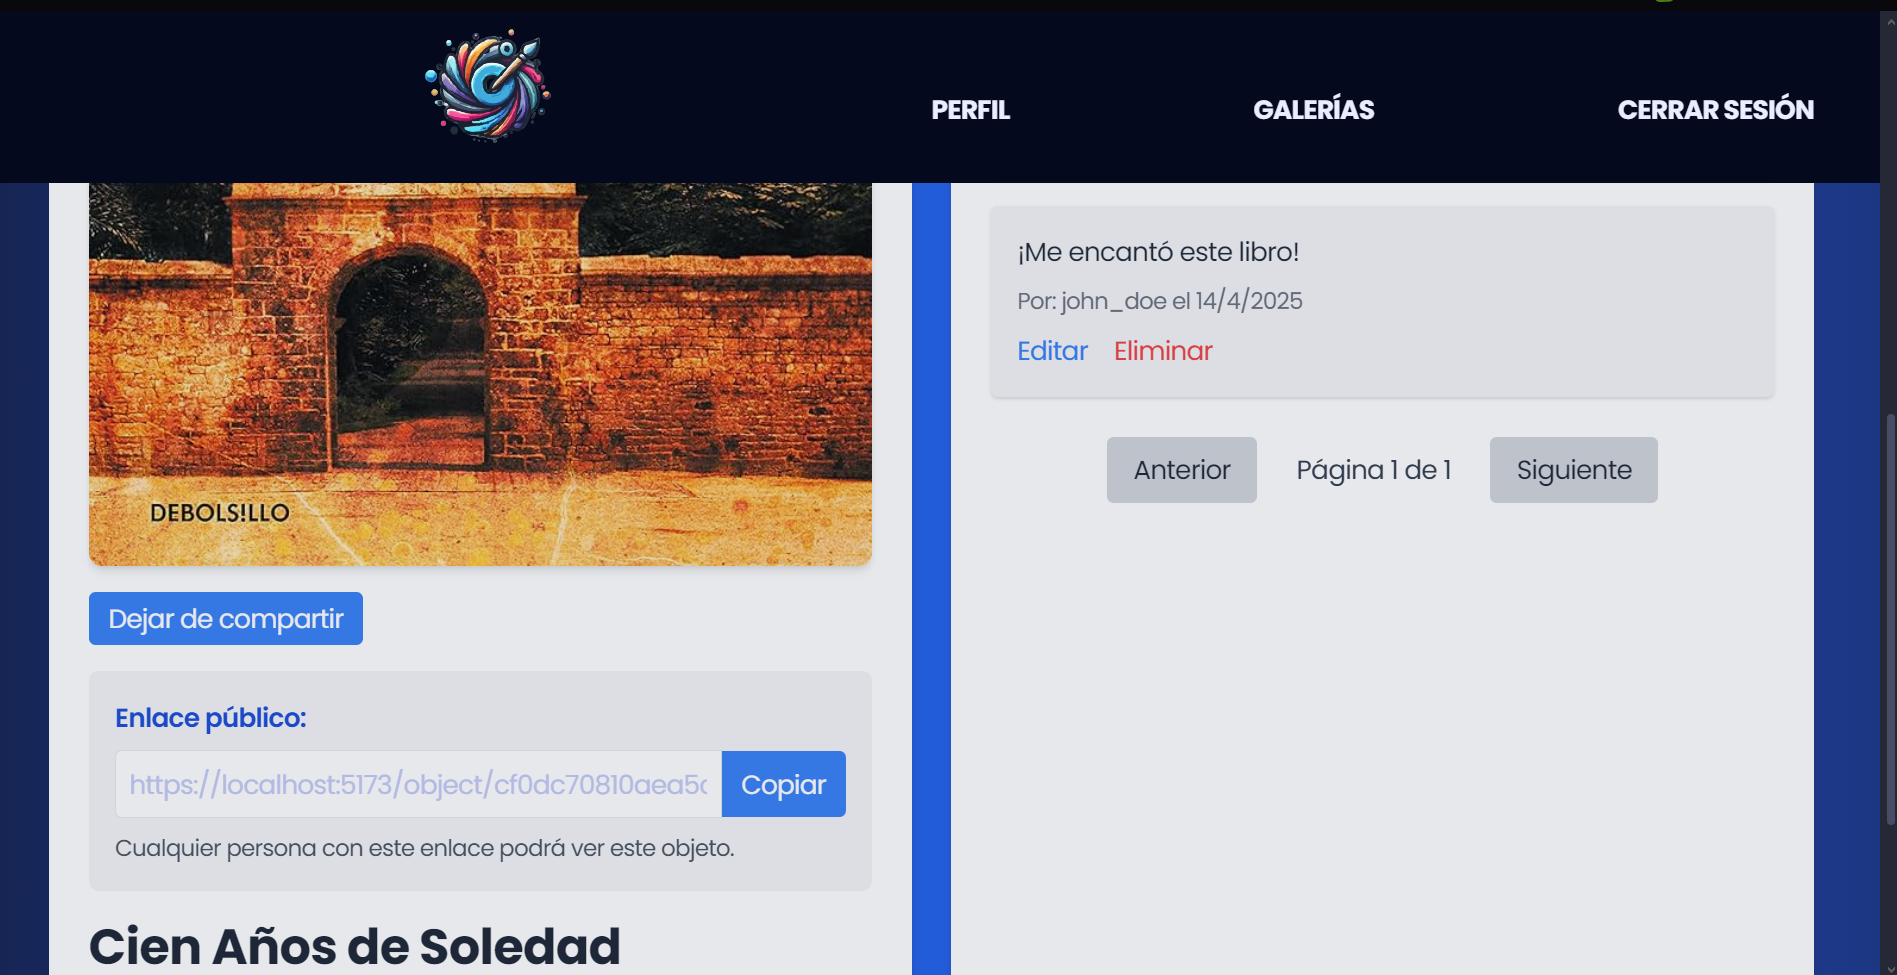
\includegraphics[clip=true,width=\textwidth]{img/share2.png}\\

    \footnotesize (k)
  \end{minipage}
  \caption{Pantalla de Objeto en Detalle.}\label{fig:pantallaObjetoDetalle}
  \end{figure}

\section{Funcionalidades Adicionales menores para Usuarios Registrados}
\label{appB:funcionalidadesAdicionales}
\begin{itemize}
    \item \textbf{Compartir Objetos:} Puede optar por hacer públicos sus objetos para que otros usuario, incluso no registrados, puedan verlos. Esta opción está disponible en la vista detallada del objeto. Al compartir, se genera un enlace único. Figura \ref{fig:pantallaObjetoDetalle}
    \item \textbf{Marcar como Favorito:} En la tarjeta de cada objeto, encontrará un icono de un corazón para marcar o desmarcar un objeto como favorito, facilitando su acceso posterior mediante el filtro de favoritos. Figura \ref{fig:pantallaGaleria}
    \item \textbf{Gestión de Perfil:} Desde el menú de navegación, puede acceder a su ``Perfil'' para actualizar su nombre, apellido, usuario, imagen de perfil y biografía.
\end{itemize}

\section{Panel de Administración (Solo para Administradores)}
\label{appB:panelAdmin}
Los usuarios con rol de administrador tienen acceso a un ``Panel de Administración'' o \textit{Dashboard} desde el menú principal. Este panel ofrece: Figura \ref{fig:pantallaDashboard}
\begin{itemize}
    \item Estadísticas sobre el uso de la plataforma (usuarios, contenido, actividad, crecimiento).
    \item Herramientas para visualizar y moderar (eliminar) todos los objetos y comentarios (una vez dentro de los objetos) de la plataforma.
    \item Una vista para gestionar usuarios.
\end{itemize}

\begin{figure}
   \centering

  \begin{minipage}{0.45\textwidth}
   \centering

     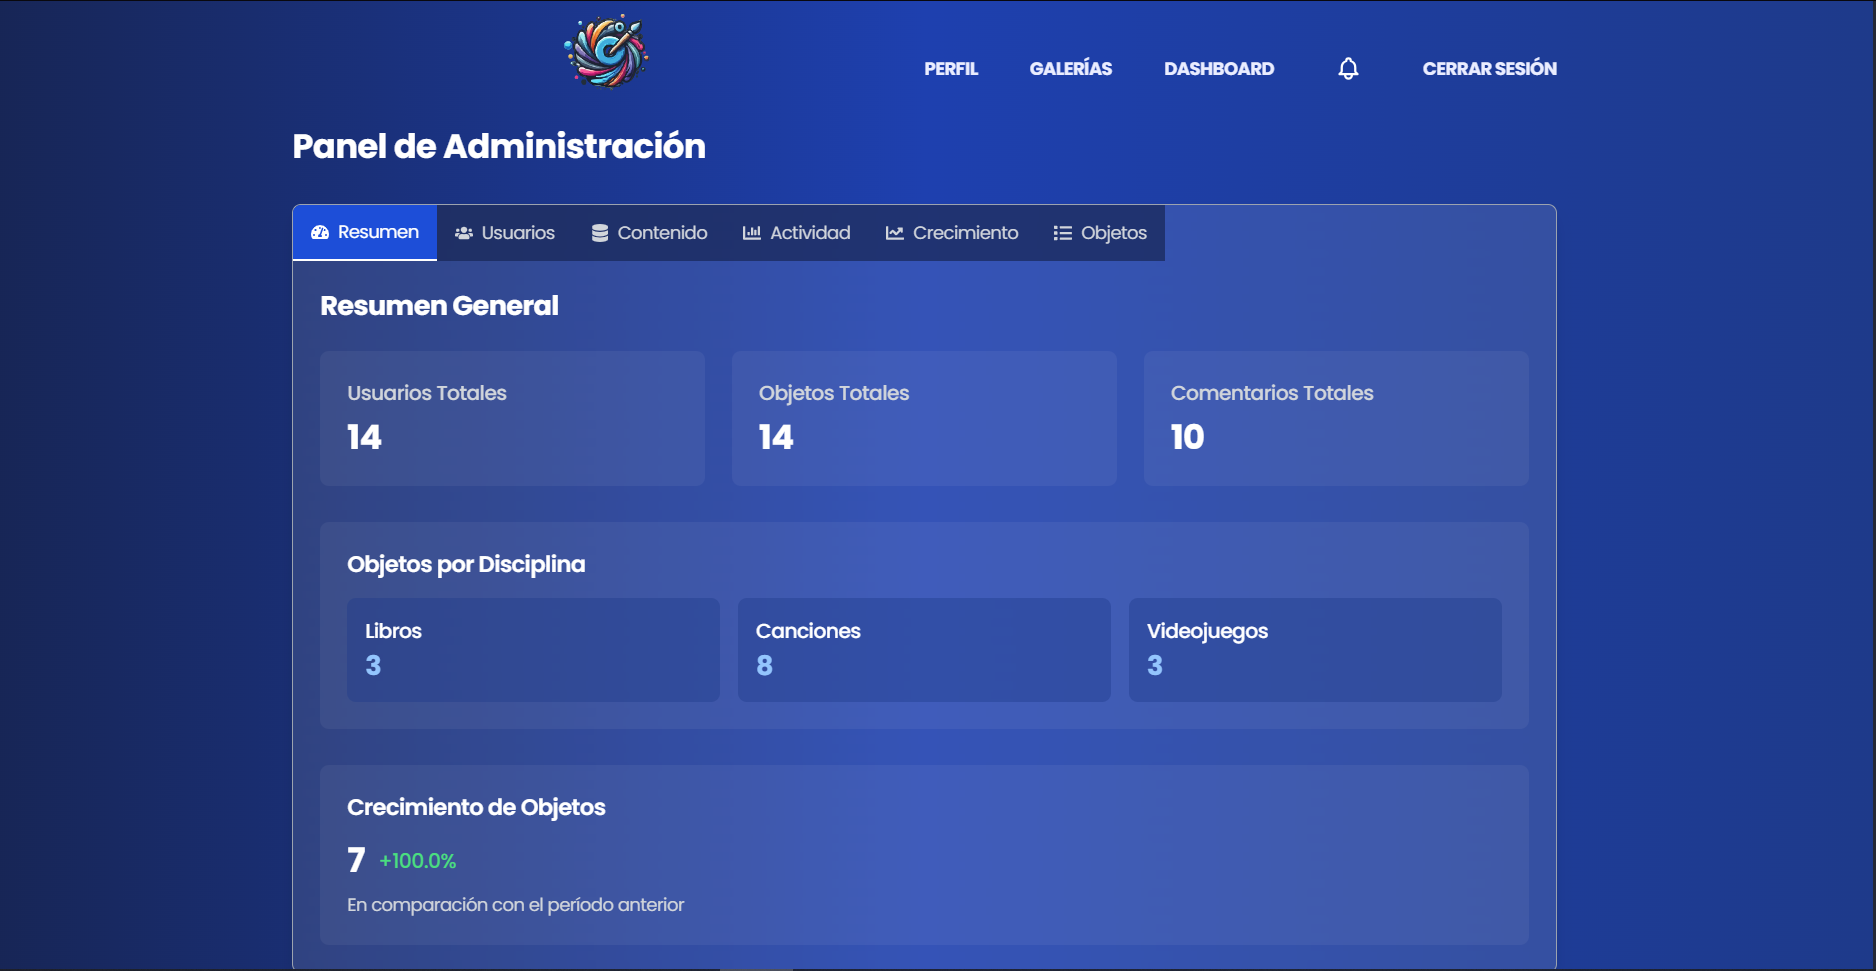
\includegraphics[clip=true,width=\textwidth]{img/dashboard2.png}\\

    \footnotesize (l)
  \end{minipage}
  \caption{Pantalla de Dashboard de Administrador.}\label{fig:pantallaDashboard}
  \end{figure}
  
El funcionamiento detallado de cada sección del dashboard es intuitivo y se presenta a través de diferentes pestañas, además de estar claramente definido en \ref{rf:adminFuncionalidades}

\section{Cierre de Sesión}
\label{appB:cierreSesion}
Para finalizar su sesión en LogArt, utilice la opción ``Cerrar Sesión'' disponible en el menú de navegación



% Fin del documento
\end{document}
